

\chapter{Introduction}

%We explore the available formalisms for design of asynchronous digital
%circuits and compare them with the principle of compositionality in
%mind. We propose improvements to the existing techniques and
%propose a new formalism, Parametrised Graph (PG) theory, which is a
%generalisation of the existing CPOG formalism. We furhter study 
%the theory of PG Algebra and present mechanised formal proofs of certain properties.


% productivity gap
The major challenge for the future of semiconductor industry is the infamous design productivity gap. This gap is caused by the exponential complexity growth of electronic systems~\cite{Moore_1965_e}  while capability of design tools cannot cope with this pace, see Fig.~\ref{fig:productivity_gap}. The only way to deal with the increasing complexity of Integrated Circuits (ICs) is to improve the efficiency of the design process, in particular, by heavily reusing system components and by advancing the design automation methods.

\begin{figure}
\centering
  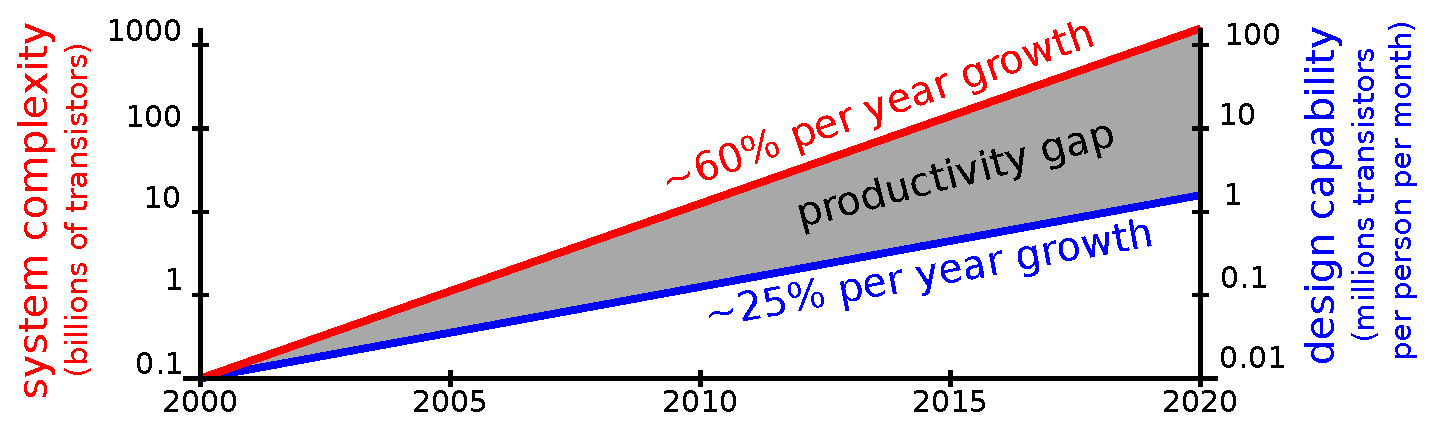
\includegraphics[scale=0.5]{fig/figs/productivity_gap}
  \caption{
    \label{fig:productivity_gap}
    Desigh productivity gap}
\end{figure}


% design reuse and need for async design principles
It has been predicted by ITRS~\cite{ITRS_2011} that in order to address the productivity gap challenge, by 2020 at least 90\% of the complex circuits should be built of previously designed components. This rises the need for compositional (or modular) design principles where the timing of individual modules is independent of the rest of the system and  therefore require delay insensitive communication between the modules. This communication discipline is natural for asynchronous circuits where the data transition is accompanied by request-acknowledgement handshaking between the sending and the receiving counterparts. On this pathway the previously designed Intellectual Property (IP) cores will need to be adapted to the new modular architectures. The least intrusive is the Globally Asynchronous Locally Synchronous (GALS) approach~\cite{Chapiro_1984_phd} where special wrappers~\cite{Mullins_2007_async, Fan_2009_iccd} are built around synchronous modules to convert their communication into asynchronous handshake style. Another alternative is desynchronisation techniques~\cite{Cortadella_2006_ieeetcad} where the global clock is replaced by a distributed control which determines when the computation is complete and the output result is ready to be consumed. This control may take different forms, from a delay line matching the critical path of the module~\cite{Cortadella_2010_icicdt} to explicitly introduced completion detection logic~\cite{Kondratyev_2002_ieeedtc}.

% synthesis of async components
The remaining 10\% of the ICs will still need to be designed from scratch. One way is to design those components in traditional synchronous way and then apply the previously discussed techniques to comply with the delay insensitive interface requirements. This, however, may result in suboptimal solutions in terms of circuit area, computation speed and energy consumption. Better results can be achieved if the components are designed and implemented with their asynchronous environment in mind~\cite{Martin_2006_ieeeproc}. However, the logic synthesis of asynchronous circuits is computationally expensive and not applicable to large modules. This is due to high level of concurrency in truly asynchronous systems which results in a state space explosion.  The computation complexity problem has been successfully addressed in the syntax-driven translation~\cite{balsa} approach which is based on direct mapping of specification into hardware components without going through the state space exploration (it is assumed that there is one-to-one correspondence between the specification language constructs and the library of available components).

% need for compositional approach
The major drawback of the circuits obtained by the syntax-driven translation is the suboptimal performance of their control structures~\cite{Plana-balsa-control-overhead}. In order to resolve this issue the control models of all the components need to be composed together and resynthesised exploiting the benefits of their joint optimisation. Existing resynthesis methods are based on parallel composition of component models expressed in form of Petri nets~\cite{carmona-handshake-clustering}. However, the efficient parallel composition of the component models is still an open question and is one of the primary goals of this thesis.

\begin{figure}
\centering
  \newcommand{\figgg}[2]{
    \subfloat[#1]{
      \label{fig:#2}
      \includegraphics[scale=0.7]{fig/figs/#2}
  }}
  \figgg{Structural composition}{composition_structural}
  \\
  \figgg{Naive behavioural composition}{composition_behavioural_naive}
  \figgg{Behavioural composition}{composition_behavioural}
  \caption{
    \label{fig:productivity_gap}
    Desigh productivity gap}
\end{figure}

% structural and behavioural aspects of composition
The composition of circuit components is of structural nature - they are combined via input-output interfaces according to the casual dependency between the operation they perform, as shown in Fig.~\ref{fig:composition_structural}.
Another compositional aspect is a combination of several mutually exclusive behaviours in the same circuit. A naive way to build such a circuit is to implement the different behaviour scenarious in separate modules and structurally compose them with the use of multiplexers and demultiplexers, as shown in Fig.~\ref{fig:composition_behavioural_naive}. A mode selection code on the (de)multiplexors determines the current scenario.  While this is a valid implementation of multi-modal functionality, it ignores the mutually exclusive feature of the implemented behaviours and looses a possibility of partial hardware reuse for common functionality, as shown in Fig.~\ref{fig:composition_behavioural}. 

A model which naturally captures the structural and behavioural aspects of composition in a single formalism is Conditional Partial Order Graphs (CPOGs)~\cite{2009_mokhov_phd}. This graph-based model is capable of expressing the structural composition by means of causality arcs (similar to Petri nets) and the behavioural composition by means of boolean "visibility" conditions on its vertices. While CPOGs is a convenient tool for reasoning on small benchmarks, it lacks the means for capturing and transformation of large systems. An ambitious goal of this thesis is to generalise the CPOGs model and introduce a theory for their manipulation in algebraic form, which is a more suitable representation for complex benchmarks.



%\section{Motivation}
%
%With constantly growing transistor counts and consumer demands, the complexity of digital circuits must grow too.
%
%With the rising complexity of digital circuits, it becomes increasingly important to reuse parts of existing designs.
%
%The reuse of the components must be facilitated by the design language.
%
%One of the difficulties in designing modern hardware systems is the
%necessity to comprehend and to deal with a very large number of system
%configurations, operational modes, and behavioural scenarios. 
%
%\subsection{Compositionality}
%
%The key property facilitating component reuse is compositionality.
%
%Compositionality is a property of a given language where the meaning of a language construct is determined by the meanings of its parts.
%

\section{Contributions}

The main contributions of the thesis are as follows:

\begin{itemize}
\item
\textbf{Improved parallel composition:} a novel method for composition of models specified with labelled Petri Nets.

\item
\textbf{Balsa circuit synthesis:} application of labelled Petri nets and parallel composition to synthesis of Balsa handshake circuits.

\item
\textbf{CPOG Synthesis:} a technique for synthesis of processor instruction decoder using instruction sets specified with Conditional Partial Order Graphs.

\item
\textbf{PG theory:} formal specification of theory of parameterised graphs with CPOGs as an example of its algebra.

\item
\textbf{CAD tool support:} automation for design of CPOGs and Balsa circuits using Workcraft framework.

\end{itemize}

\section{Structure}

The rest of the thesis is organised as follows:

Chapter~\ref{chap:Background} covers the basics of handshake circuits, signal transition graphs and conditional partial order graphs.

Chapter~\ref{chap:Approach} overviews the contributions of the thesis in more detail by discussing the contribution of every chapter and the way they relate to each other.

Chapter~\ref{chap:ParComp} describes the proposed improved parallel composition algorithm. The contents of this chapter is based on the results published previously in \cite{improved_par_comp}.

Chapter~\ref{chap:PGAlgebra} introduces Parametrised Graph (PG) theory, defining and studying an algebraic structure that generalises Conditional Partial Order Graph formalism. This chapter is based on the results previously published in~\cite{pg_algebra}.

Chapter~\ref{chap:PGEncoding} describes a technique for optimal encoding of processor instruction sets defined using TPG formalism. This chapter is based on the results previously published in~\cite{cpog_encoding_best_paper} and~\cite{cpog_encoding}. The former has qualified for a best paper award at the ACSD conference.

Chapter~\ref{chap:Conclusion} summarises the achieved results and proposes ideas for future research.

\chapter{Background}

\label{chap:Background}
This chapter introduces a brief overview of the major techniques and models used throughout the thesis. In particular, handshake circuits -- a specification formalism for synthesis of self-timed hardware; Petri nets -- a graph-based notation for reasoning about concurrent behaviour; conditional partial order graphs (CPOG) -- a versatile notation for describing a family of partial orders.


\section{Handshake circuits}


One of the approaches to design of asynchronous circuits is syntax-directed mapping with 
handshake circuits as an intermediate format. The parse tree of a program source code written in 
a CSP-style \cite{csp} language can be interpreted as a graph of components, connected with communication links
called handshake channels. The components can then be individually mapped to gate-level implementations
with complete circuit derived by implementing the handshake channels with wires.

This approach has been first used by Philips in their Tangram \cite{tangram} design tool
and later made publicly available after the similar free Balsa \cite{balsa} system has been released.

This thesis will be working with Balsa handshake components.

A handshake activation $h$ is said to \emph{enclose} a process $p$ if $p$ can only start after $h$ gets a request and $h$ can get an acknowledgement only after $p$ gets finished.

A \emph{handshake circuit} consists of handshake components which interact by request/acknowledgement handshaking 
over communication channels.
Each \emph{handshake component} is specified by a set of ports and a process communicating over those ports.
A \emph{protocol} is assigned to each port, which specifies whether the process initiates the handshakes
over an \emph{active port} or awaits for the other party over a \emph{passive port}. 
It also specifies the direction and size of data transferred during the handshakes.
Each \emph{channel} connects two ports of the same data size with one port being active and the other being passive.

On diagrams used in this thesis we display handshake components with large circles with a process symbol inside
and handshake ports with small circles where filled circle stands for active port and hollow circle stands for passive port.
Channels are displayed as lines between the corresponding ports with the direction of the arrow corresponding to the
direction of data flow.


The defining feature of a handshake component is the process associated with it. 
In Balsa there are about fifty types of processes with each 


\begin{itemize}
\item
Sequence is a component with three control ports: a passive port $s$ and two active ports $t_1$ and $t_2$.
The behaviour of the component is as follows: upon receiving an activation it encloses the two activations activation of $t_1$ action   awaits for activation over $s$ and encloses the following: a handshake over $activate_1$ followed by a handshake over $activate_2$; after receiving the acknowledgement  and acknowledges

\item
Concur is a component with a similar external interface: it has a passive port $activate$ and two active ports $activate_1$ and $activate_2$.
The behaviour during the activation on $activate$ is to activate $activate_1$ and $activate_2$ concurrently.

\item
Sync is a component with three control ports: two passive ports s_1 and s_2 and an active port t. 
This component ensures that $t$ is enclosed 
\end{itemize}



\begin{figure}
\centering
\subfloat[Sequence\label{fig:SequenceOptimised}]{
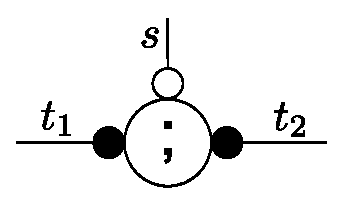
\includegraphics[scale=0.5]{figures/Control/sequence-HC}
} {}
\subfloat[Concur\label{fig:Concur}]{
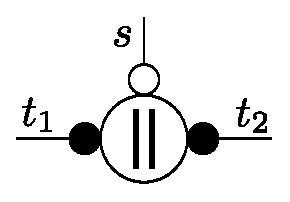
\includegraphics[scale=0.5]{figures/Control/concur-HC}
} {}
\subfloat[BinaryFunc\label{fig:BinaryFunc}]{
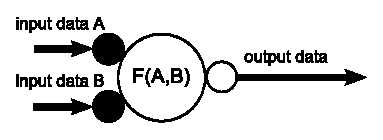
\includegraphics[scale=0.4]{figures/Data/binaryfunc-HC}
} {}
\subfloat[CallMux\label{fig:CallMux}]{
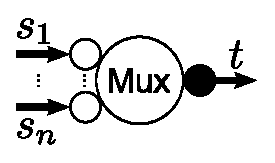
\includegraphics[scale=0.5]{figures/Data/callmux-HC}
} {}
\subfloat[Variable\label{fig:Variable}]{
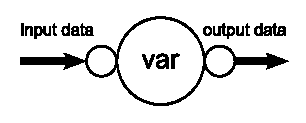
\includegraphics[scale=0.5]{figures/Data/variable-HC}
} {}
\subfloat[While\label{fig:While}]{
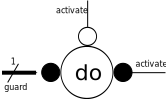
\includegraphics[bb=0bp 0bp 134bp 80bp,scale=0.5]{figures/while-HC}
} {}
\subfloat[Case\label{fig:Case}]{
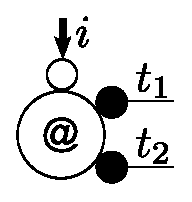
\includegraphics[scale=0.5]{figures/case-HC}
}

\caption{Handshake components}
\end{figure}





 Each channel connects two ports. Each port is connected to a channel. 
with which it
can be connected point-to-point to a port of another handshake circuit by means of a channel. 
. Each
channel carries request and acknowledgement signalling as well as an optional data payload. The
requests flow from the active component ports (filled circles) towards passive component ports
(open circles). Acknowledgements flow in the opposite direction to requests. Where a channel
carries data, the direction of the data is indicated by an arrow on that channel’s arc. The direction
of data may be different from the direction of signalling to support push and pull port and channels.
A handshake component can be activated by sending request to its passive port. When activated, 
it sends requests to a subset of its active ports and waits for acknowledgements. The
subset of the ports activated by the component is determined by its function and may be data-
dependent. The order in which the component activates its ports is shown by small numbers next
to the ports. The ports of a handshake component which are marked with the same number are ac-
tivated concurrently. When all activated ports are acknowledged, the handshake component sends
an acknowledgement to the passive port from which it was activated and finishes its operation until
the next activation.

\section{Improved Parallel Composition}\label{sec_intro}



\subsection{Abstract}
Parallel composition of labelled Petri nets is a fundamental operation in modular design. It is often used to combine models of subsystems into a model of the whole system.
Unfortunately, the standard definition of parallel composition almost always yields a `messy' Petri net, with many implicit places, causing performance deterioration in tools that are based on structural methods. In this paper we propose an optimised algorithm for computing the parallel composition. It often produces nets with fewer implicit places, which are thus better suited for subsequent application of structural methods.

\subsection{Introduction}

Parallel composition (\aka synchronous product) of labelled
Petri nets is a fundamental operation in modular design. It is
often used to combine models of subsystems into a model of the
whole system. In particular, there is a nice correspondence
between parallel composition of Signal Transition Graphs
(STGs), a class of labelled Petri nets used for modelling
asynchronous circuits, and connecting circuits by wires. Hence
performing this operation efficiently is important in practice.

Unfortunately, the standard definition of parallel composition almost always yields a `messy' Petri net, with many implicit places (even if the component Petri nets did not have them). Some of these places are easy to remove (\eg duplicate places, which have the same pre- and postsets), but in general for removing others one needs full-blown model checking, which is infeasible if the resulting composition is large.
Although implicit places do not have noticeable effect on tools based on state space exploration, such as \petrify~\cite{ckkly97}, the performance of tools that are based on structural methods, such as \desij~\cite{Sch07}, often deteriorates.

Consider an example shown in Fig.~\ref{fi-motivating-example1},
which shows the STG specifications of two components (a,b) and
the specification of the environment (c). (The used short-hand
drawing notation for STGs is explained in
Sect.~\ref{sec_pn_basic}.) The model of the behaviour of the
entire system can be obtained by constructing the parallel
composition of these three STGs, which is shown in part (d) of
this figure. One can see that it contains a few implicit places
(which are not duplicate places); intuitively, they appear due
to repeated causality specifications for every signal: the one
coming from the component where this signal is an output, and
others --- from the components where it is an input. Removing
these places yields a much `cleaner' STG, coinciding with that
shown in Fig.~\ref{fi-motivating-example2}(d).

\begin{figure}[!tb]
    \centering
    \begin{minipage}[b]{0.4\columnwidth}
    \centering
        $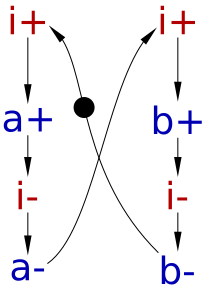
\includegraphics[scale=0.3]{EXPERIMENTS/stg/toggle}
        \atop
        \mbox{\rule[1.3em]{0em}{0em}(a) Toggle}$
        \\[0.5em]
        $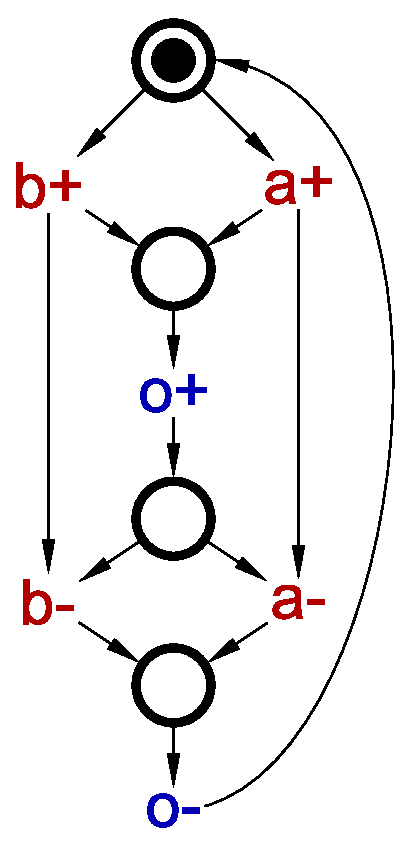
\includegraphics[scale=0.3]{EXPERIMENTS/stg/mix}
        \atop
        \mbox{\rule[1.3em]{0em}{0em}(b) Call}$
        \\[0.5em]
        $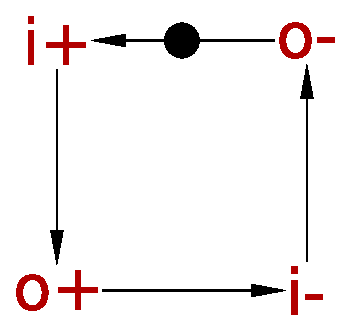
\includegraphics[scale=0.3]{EXPERIMENTS/stg/env}
        \atop
        \mbox{\rule[1.3em]{0em}{0em}(c) Environment}$
    \end{minipage}
    $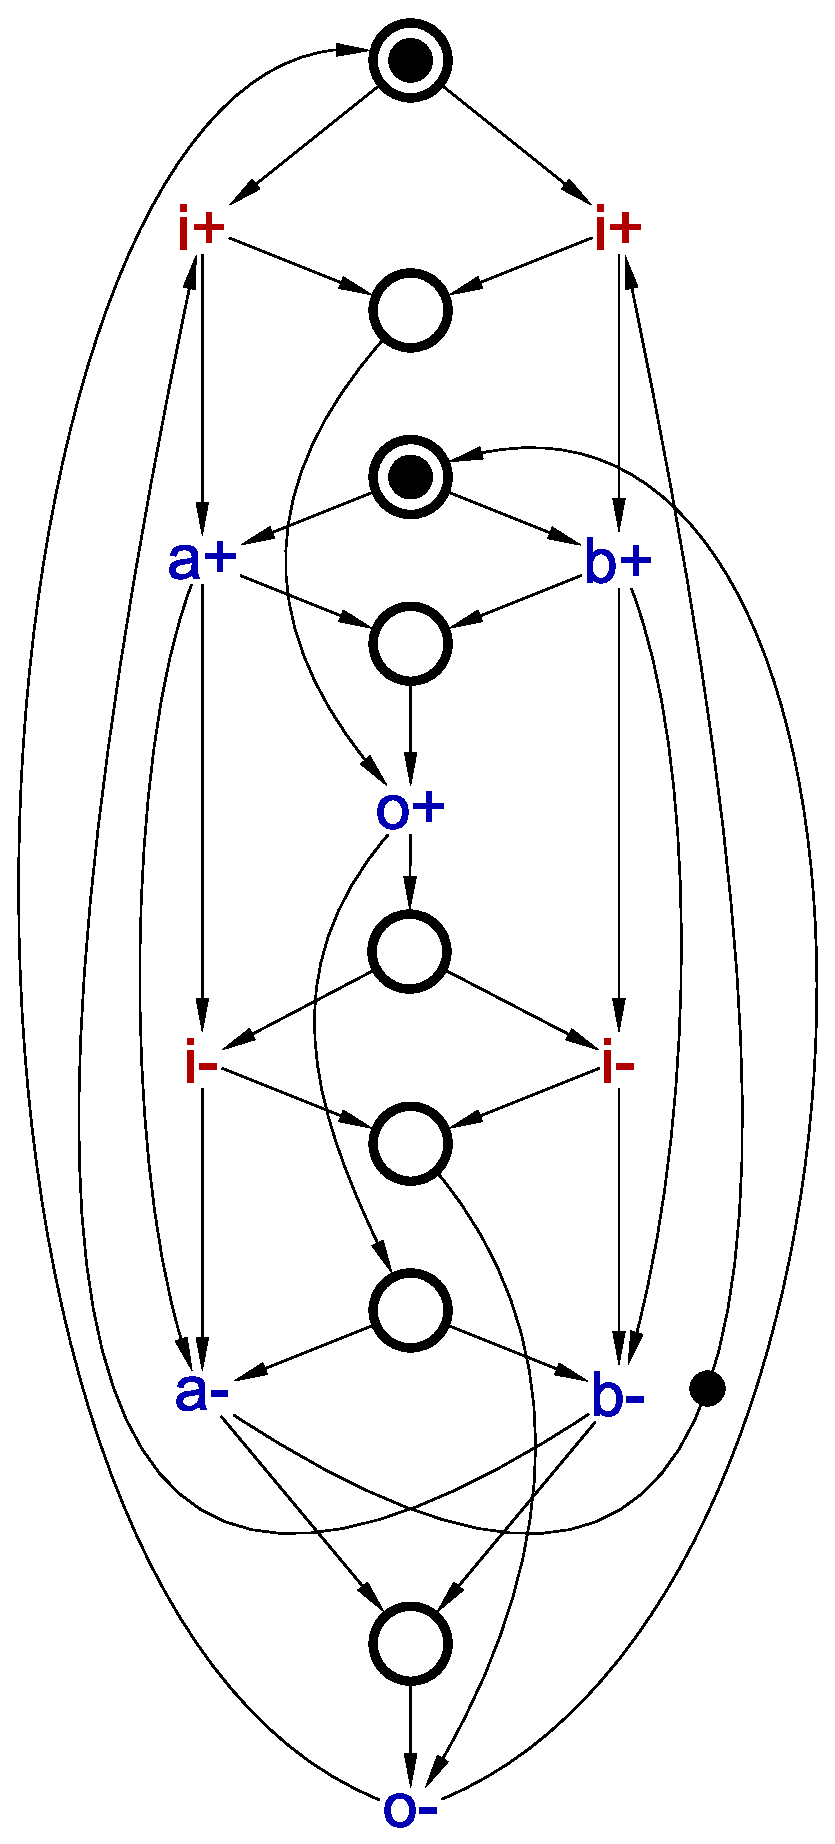
\includegraphics[scale=0.3]{EXPERIMENTS/stg/simple_standard}
    \atop
    \mbox{\rule[1.3em]{0em}{0em}(d) Composition}$
    \caption{\label{fi-motivating-example1}
        Example of standard STG composition.
    }
\end{figure}

\begin{figure}[!tb]
    \centering
    \begin{minipage}[b]{0.4\columnwidth}
        \centering
        $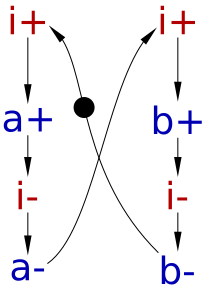
\includegraphics[scale=0.3]{EXPERIMENTS/stg/toggle_opt}
        \atop
        \mbox{\rule[1.3em]{0em}{0em}(a) Toggle}$
        \\[0.5em]
        $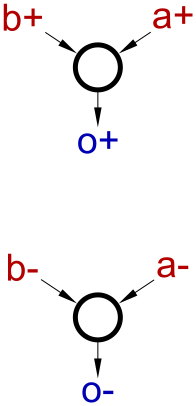
\includegraphics[scale=0.3]{EXPERIMENTS/stg/mix_opt}
        \atop
        \mbox{\rule[1.3em]{0em}{0em}(b) Call}$
        \\[0.5em]
        $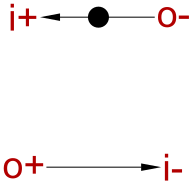
\includegraphics[scale=0.3]{EXPERIMENTS/stg/env_opt}
        \atop
        \mbox{\rule[1.3em]{0em}{0em}(c) Environment}$
    \end{minipage}
    $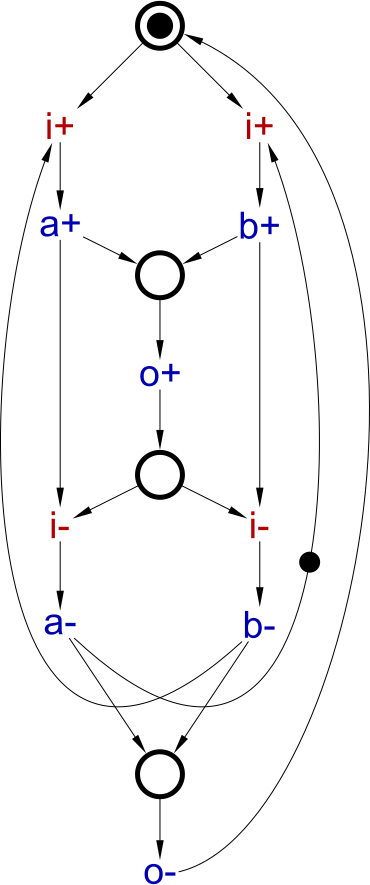
\includegraphics[scale=0.3]{EXPERIMENTS/stg/simple_improved}
    \atop
    \mbox{\rule[1.3em]{0em}{0em}(d) Composition}$
    \caption{\label{fi-motivating-example2}
        Example of improved STG composition: the components are obtained from the corresponding ones in Fig.~\ref{fi-motivating-example1} by removing some places, and then the standard parallel composition is applied to these modified components.
    }
\end{figure}


One operation where implicit places matter is \emph{transition contraction,}~\cite{vowo02lncs} which is a crucial part of the re-syn\-the\-sis approach~\cite{CN-02,KVL-96,PC-96}. The idea is to hide the internal communication between the components (by labelling the corresponding transitions as `dummy' --- they correspond to signals $a$ and $b$ in our example), contract as many of these dummy transitions as possible (whereby reducing the size of the STG), and re-synthesise the obtained STG as a circuit (which is often smaller than the original circuit due to removal of some signals). Transition contraction has to be performed on very large STGs (corresponding to the whole control path of the circuit), and so, for efficiency, it has to be a structural operation. Unfortunately, such structural contractions are not always possible (see Sect.~\ref{sec_pn_basic}), and implicit places in the preset and/or postset of a transition can prevent contracting it, even if a contraction is possible after removing these implicit places. In our example, \desij cannot contract any of the dummy transitions in the STG in Fig.~\ref{fi-motivating-example1}(d), even though it performs some structural tests for place redundancy; however, it is able to contract all the dummy transitions if the implicit places are removed, \ie when applied to the STG in Fig.~\ref{fi-motivating-example2}(d).

The main contribution of this paper is a new me\-thod for computing the parallel composition of labelled Petri nets, that generates fewer implicit places. It uses the \emph{freeness from computation interference (FCI)} assumption, stating that the situation when one component wants to produce an output, but is prevented from doing so by another component which is not ready to receive it, is impossible. Violation of FCI means that the behaviour of the composition does not correspond to that of the physical system. For example, an output of a circuit component cannot be physically disabled by another component that is not ready to receive this signal, and so producing this output will lead to malfunction; however, the composition will be oblivious to it, and behave as if such an output could not be produced.
Hence FCI is a basic correctness requirement --- if it is violated, there is no point in computing parallel composition, as its behaviour will not describe that of the physical system. In practice, FCI is often guaranteed by construction, \eg it is always guaranteed for the control path of a \balsa~\cite{EB-02} or \haste/\tangram~\cite{berkel91,haste-manual} specification of an asynchronous circuit. The idea of using the FCI condition is reminiscent of the method of input/output exposure in the synthesis by direct mapping described in~\cite{SBY-07}, and of the correct by construction composition of Petri nets for circuit components and the environment used in the \ditopn tool~\cite{JF-00}.

The main idea of the method we propose here is illustrated by the example in Fig.~\ref{fi-motivating-example2}. Before doing the parallel composition, one can remove some of the places in the components as shown in parts (a--c) of the figure and then compose the modified STGs. The precise conditions that allow to remove a particular place will be stated in Sect.~\ref{se-main}; at this point it is only important that they are structural and thus can be efficiently checked. This guarantees that the number of places in the resulting Petri net is smaller (as the number of places in the composition is the total number of places in all the components), and, under the FCI assumption, the resulting behaviour will be the same (in the sense of isomorphism of the reachability graphs). In particular, in our example, composing the modified components yields the STG in Fig.~\ref{fi-motivating-example2}(d), which in this case contains no implicit places. Observe that the modified components on their own can have rather bad behaviour and in particular can be non-implementable; however, it does not matter, as they are never used on their own, but only in composition with other components, and the resulting behaviour of the composition is guaranteed to correspond to that of the standard composition.

Re-synthesis of asynchronous circuits is the intended application of the proposed method. However, we envisage that it has a much wider applicability, as composition of labelled Petri nets is a fundamental operation, and the FCI assumption often holds in practice.

\section{Conditional Partial Order Graphs\label{sec:CPOG-model-essentials}}

A \emph{Conditional Partial Order Graph}~\cite{2009_mokhov_phd}\cite{2010_mokhov_ieee}
is a quintuple $H=(V,\ E,\ X,\ \rho,\ \phi)$, where $V$ is a finite
set of \emph{vertices}, $E\subseteq V\times V$ is a set of \emph{arcs}
between them, and $X$ is a finite set of \emph{operational}\emph{variables}. An \emph{opcode} is an assignment $(x_{1},\ x_{2},\ \dots,\ x_{|X|})\in\{0,\ 1\}^{|X|}$
of these variables; $X$ can be assigned only those opcodes which
satisfy the \emph{restriction function} $\rho$
of the graph, i.e. $\rho(x_{1},\ x_{2},\ \dots,\ x_{|X|})=1$. Function
$\phi$ assigns a Boolean \emph{condition} $\phi(z)$ to every vertex
and arc $z\in V\cup E$ of the graph.

\begin{figure}[h]
\hfill{}\subfloat[Full notation]{

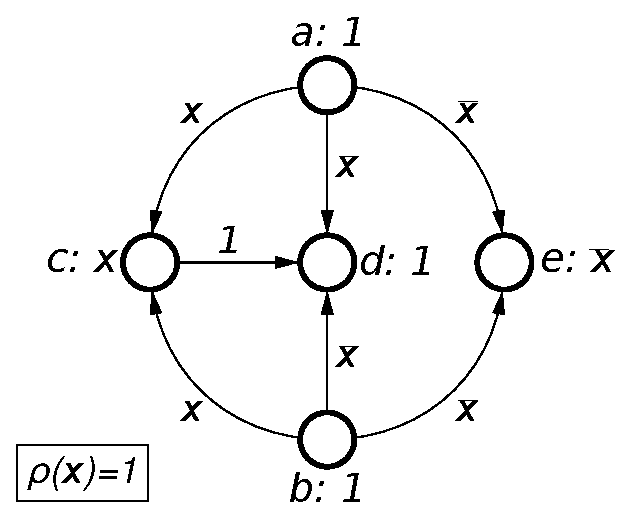
\includegraphics[scale=0.45]{fig/cpog}}\hfill{}\subfloat[Simplified notation]{

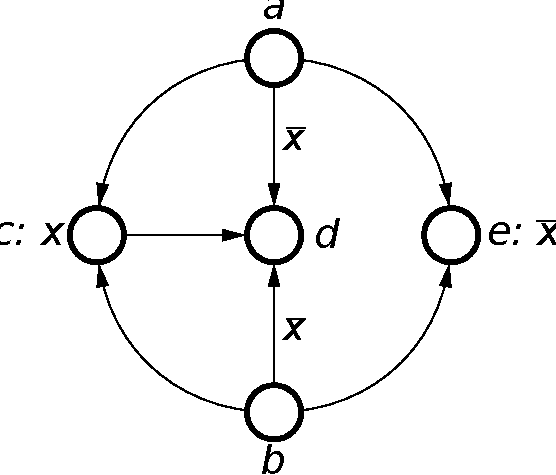
\includegraphics[scale=0.45]{fig/cpog_simplified}}\hfill{}

\begin{centering}
\subfloat[Multiple CPOG projections]{\begin{centering}
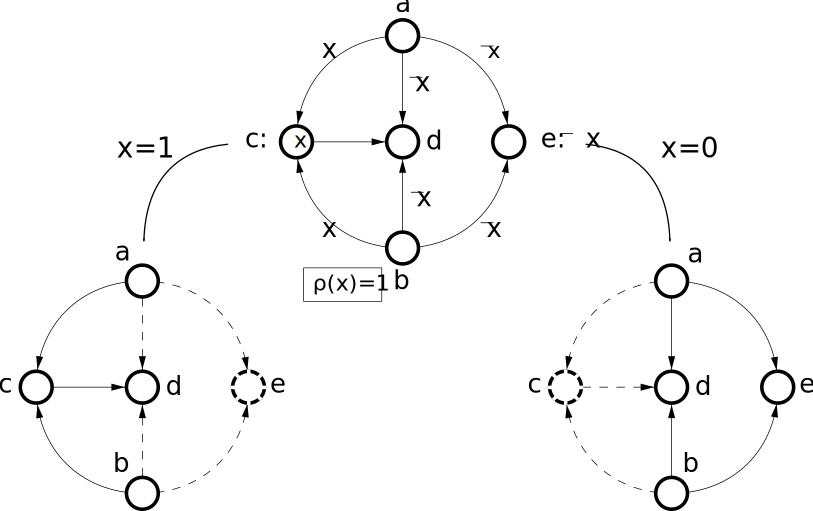
\includegraphics[scale=0.45]{fig/cpog_projections_2}
\par\end{centering}

}
\par\end{centering}

\caption{\label{fig-cpog-examples}Graphical representation of CPOGs and their projections}
\end{figure}


Figure~\ref{fig-cpog-examples}(a) shows an example of a CPOG containing
$|V|=5$ vertices and $|E|=7$ arcs. There is a single operational
variable $x$; the restriction function is $\rho(x)=1$, hence both
opcodes $x=0$ and $x=1$ are allowed. Vertices $\{a,\ b,\ d\}$ have
constant $\phi=1$ conditions and are called \emph{unconditional},
while vertices $\{c,\ e\}$ are \emph{conditional} and have conditions
$\phi(c)=x$ and $\phi(e)=\overline{x}$ respectively. Arcs also fall
into two classes: unconditional (arc $c\rightarrow d$) and conditional
(all the rest). As CPOGs tend to have many unconditional vertices
and arcs we use a simplified notation in which conditions equal to
$1$ are not depicted in the graph. This is demonstrated in Figure~\ref{fig-cpog-examples}(b).

The purpose of conditions $\phi$ is to `switch off' some vertices
and/or arcs in the graph according to the given opcode. This makes
CPOGs capable of specifying multiple partial orders or instructions
(a partial order is a form of behavioural description of an instruction).
Figure~\ref{fig-cpog-examples}(c) shows a graph and its two \emph{projections}.
The leftmost projection is obtained by keeping in the graph only those
vertices and arcs whose conditions evaluate to $1$ after substitution
of the operational variable $x$ with $1$. Hence, vertex $e$ disappears,
because its condition evaluates to $0$: $\phi(e)=\overline{x}=\overline{1}=0$.
Arcs $\{a\rightarrow d,\ a\rightarrow e,\ b\rightarrow d,\ b\rightarrow e\}$
disappear for the same reason. The rightmost projection is obtained
in the same way with the only difference that variable $x$ is set
to $0$. Note also that although the condition of arc $c\rightarrow d$
evaluates to $1$ (in fact it is constant $1$) the arc is still excluded
from the resultant graph because one of the vertices it connects (vertex
$c$) is excluded and obviously an arc cannot appear in a graph without
one of its vertices. Each of the obtained projections can be treated
as a specification of a particular behavioural scenario of the modelled
system. Potentially, a CPOG $H=(V,\ E,\ X,\ \rho,\ \phi)$ can specify
an exponential number of different partial orders of events in $V$
according to one of $2^{|X|}$ different possible opcodes.

A CPOG is \emph{well-defined} if all its projections allowed by
$\rho$ are acyclic. We consider only well-defined CPOGs in this thesis,
because a cyclic projection has no natural execution semantics, in
particular it is not clear which event can be executed first unless
some form of a \textquoteleft{}token\textquoteright{} is introduced
as in the Petri Net model~\cite{2002_cortadella_book}.

To summarise, a CPOG is a structure to represent a set of encoded
partial orders in a compact form. Synthesis and optimisation methods
presented in~\cite{2010_mokhov_ieee} provide a way to obtain such
a representation given a set of partial orders and their opcodes.
For example, the CPOG in Figure~\ref{fig-cpog-examples}(c) can be
synthesised automatically from the two partial orders below it and
the corresponding opcodes $x=1$ and $x=0$. The next section shows
that a particular assignment of opcodes to the partial orders has
a strong impact on the final CPOG, therefore in order to obtain the
most compact CPOG representation one has to search for the best opcode
assignment.

Note that partial orders is not the only formalism for formal specification
of instructions. In particular, there is an alternative approach~\cite{1994_baranov_book}
based on automata, which treats every instruction as a burst-mode
state machine and defines an operation of composition on them. While
benefiting from a direct correspondence between flowcharts of algorithms
and automata, the approach cannot model true concurrency: a set of
causally independent events can only be executed as a `burst' in
the same step/clock cycle. Also, it requires explicit memory to track
the current state of the automaton. We believe that partial orders
are better suited for modelling instruction sets of processing units
built on heterogeneous platforms, i.e. exhibiting both asynchronous
and synchronous interactions~\cite{2011_mokhov_tr}.

\input{agda-background-body}

\chapter{Approach\label{chap:Approach}}

The subject of this thesis is the advancement of compositional techniques for circuit synthesis. We start by discusssing our contribution to the compositional circuit synthesis based on STGs and present the resynthesis technique. Next we introduce the parametrised graphs formalism naturally supporting compositional reasoning. 


\section{Overview}
Handshake circuits are widely applied in the design and synthesis of real-life hardware.
One prominent problem is obtaining an efficient implementation from a \emph{structural} compositional specification.
Syntax-based synthesis tools such as Balsa~\cite{balsa} are unable to take into account the compositional
behaviour of STGs corresponding to handshake circuit components. To address this issue we propose 
a technique that selectively composes STGs of related components to obtain a smaller and more performant
circuit without suffering state space explosion commonly associated with Petri net based techniques~\cite{Valmari}.
This transformation, which we refer to as \emph{resynthesis}~\cite{ukaf_balsa_resynthesis}, is accomplished in three stages. First, we apply a heuristic to identify the most promising candidates for STG-level composition. Second, we perform a parallel composition of the selected component STGs and as a result obtain a new handshake circuit with custom components, functionally equivalent to a combination of elementary components. Finally, a gate-level implementation is obtained from the new handshake circuit via a component-wise synthesis of STGs.

Unfortunately, the standard definition of parallel composition almost always yields a `messy' Petri net, with many implicit places, causing performance deterioration in techniques that are based on structural methods such as the resynthesis approach. To counter this, we propose an improved algorithm for computing the parallel composition. The algorithm generally produces nets with fewer implicit places that are better suited for subsequent application of structural methods~\cite{improved_par_comp}.

In addition to purely structural composition of STGs, it is also beneficial to consider a mixture of 
structural and behavioural composition. Conditional Partial Order Graphs (CPOG)~\cite{2009_mokhov_phd} is a graph-based notation supporting compact
representation and efficient manipulation of both structural and behavioural composition styles. As one example, when developing complex circuit, it is
often necessary to consider several operational modes of a circuit. 
For this, one needs methodologies and tools to exploit similarities between
the individual modes and hence lift the level of discourse to behaviour families.
This necessitates that behaviours are managed in a compositional
way: the specification of the system must be composed from specifications
of its blocks. Furthermore, since the approach is intended to be a part of a safety critical toolchain, it is essential that such a  specification is amenable to mechanised reasoning and transformation.

In Chapter~\ref{chap:PGAlgebra} we propose an extension of the CPOG formalism, called Parameterised Graph (PG).
PGs deal with general graphs rather than just partial orders. We introduce an algebra of Parameterised Graphs by specifying the
equivalence relation via a set of axioms, which we prove to be sound,
minimal and complete~\cite{pg_algebra}. This result allows one to manipulate a PG model
as an algebraic expression applying the bi-directional rewrite rules of this algebra. This is  in contrast to the CPOG formalism that does not offer a unifying algebraic structure. We demonstrate
the usefulness of the developed formalism with two case studies coming
from the area of microelectronics design.

The CPOG formalism can be applied to merge several distinct behaviours
into a single compact CPOG~\cite{2009_mokhov_phd}. As one example, this has been previously used to
synthesise control logic for instruction decoding. In this thesis (Chapter~\ref{chap:PGEncoding}) 
we improve upon this work by offering a powerful technique to automatically discover an optimal encoding and
synthesise a matching optimal decoding circuit. From the outset, we consider a larger set of potential solutions
which enables us to formulate the global optimality criterion. We use an automated satisfiability solving 
techniques to find an optimal solution~\cite{cpog_encoding}.


\section{Balsa Resynthesis\label{sec:Balsa-Introduction}}

The main obstacle for the wider acceptance of asynchronous systems is the inherent complexity of their design. Several solutions are
accepted by the industry to help to simplify the design process through abstraction
of predesigned asynchronous circuit parts as standardised high level
components. A designer is able to use these components as ``building
blocks'', and then obtain the final gate-level design through an
automated mapping process. Some of the well-known asynchronous
design automation packages, such as Tangram~\cite{951597}, and Balsa~\cite{balsa},
define a high-level programming-like language that is used to describe
systems. The language constructs are then directly translated into
a network of \emph{handshake components}-- blocks with predefined
functionality that use \emph{handshakes} to interface with other components,
which are in turn mapped into a gate netlist ~ \cite{XXXX}. 

Although this method greatly enhances the designer's productivity,
it has several important drawbacks. Of these, the control-path overhead
is the most decisive. The controllers obtained by syntax-directed
mapping are usually far from optimal because the predesigned components
are required to implement their declared protocols fully and correctly
in order to be reusable in all possible circuit configurations. However,
it is often the case that a significant part of their functionality
becomes redundant due to the peculiarities of the specific configuration,
e.g. in many cases full handshaking between the components can be
avoided.

This redundancy may be eliminated by replacing a manually designed
gate-level implementation of the high level components with an equivalent
STG~(signal transition graph) specification~\cite{Yakovlev_1998_cs}.
The STGs of individual components are then composed together to form a
 STG representation of the whole system STG~\cite{785214} and is optimised with \noun{petrify~}\cite{cortadella_petrify}.
An optimal gate-level implementation is then automatically produced
from the STG using tools such as \noun{petrify}~\cite{cortadella_petrify},
\noun{SIS}~\cite{Sentovich:M92/41} and \noun{MPSat}~\cite{Khomenko_2004_MPSAT}.
Automatic synthesis becomes problematic when the size of a STG becomes
large: modern synthesis tools can handle STGs of no more than 100
signals. The impact of this problem can be lessened by including STG decomposition tools~\cite{DesiJ} into the workflow. They break a large, optimised STG down into several smaller STGs that are synthesisable
in reasonable time. Alternatively, the decomposition step is carried
out at the level of handshake circuits, dividing a circuit into several
smaller blocks of components.

\section{Improved Parallel Composition}\label{sec_intro}



\subsection{Abstract}
Parallel composition of labelled Petri nets is a fundamental operation in modular design. It is often used to combine models of subsystems into a model of the whole system.
Unfortunately, the standard definition of parallel composition almost always yields a `messy' Petri net, with many implicit places, causing performance deterioration in tools that are based on structural methods. In this paper we propose an optimised algorithm for computing the parallel composition. It often produces nets with fewer implicit places, which are thus better suited for subsequent application of structural methods.

\subsection{Introduction}

Parallel composition (\aka synchronous product) of labelled
Petri nets is a fundamental operation in modular design. It is
often used to combine models of subsystems into a model of the
whole system. In particular, there is a nice correspondence
between parallel composition of Signal Transition Graphs
(STGs), a class of labelled Petri nets used for modelling
asynchronous circuits, and connecting circuits by wires. Hence
performing this operation efficiently is important in practice.

Unfortunately, the standard definition of parallel composition almost always yields a `messy' Petri net, with many implicit places (even if the component Petri nets did not have them). Some of these places are easy to remove (\eg duplicate places, which have the same pre- and postsets), but in general for removing others one needs full-blown model checking, which is infeasible if the resulting composition is large.
Although implicit places do not have noticeable effect on tools based on state space exploration, such as \petrify~\cite{ckkly97}, the performance of tools that are based on structural methods, such as \desij~\cite{Sch07}, often deteriorates.

Consider an example shown in Fig.~\ref{fi-motivating-example1},
which shows the STG specifications of two components (a,b) and
the specification of the environment (c). (The used short-hand
drawing notation for STGs is explained in
Sect.~\ref{sec_pn_basic}.) The model of the behaviour of the
entire system can be obtained by constructing the parallel
composition of these three STGs, which is shown in part (d) of
this figure. One can see that it contains a few implicit places
(which are not duplicate places); intuitively, they appear due
to repeated causality specifications for every signal: the one
coming from the component where this signal is an output, and
others --- from the components where it is an input. Removing
these places yields a much `cleaner' STG, coinciding with that
shown in Fig.~\ref{fi-motivating-example2}(d).

\begin{figure}[!tb]
    \centering
    \begin{minipage}[b]{0.4\columnwidth}
    \centering
        $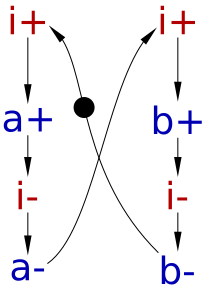
\includegraphics[scale=0.3]{EXPERIMENTS/stg/toggle}
        \atop
        \mbox{\rule[1.3em]{0em}{0em}(a) Toggle}$
        \\[0.5em]
        $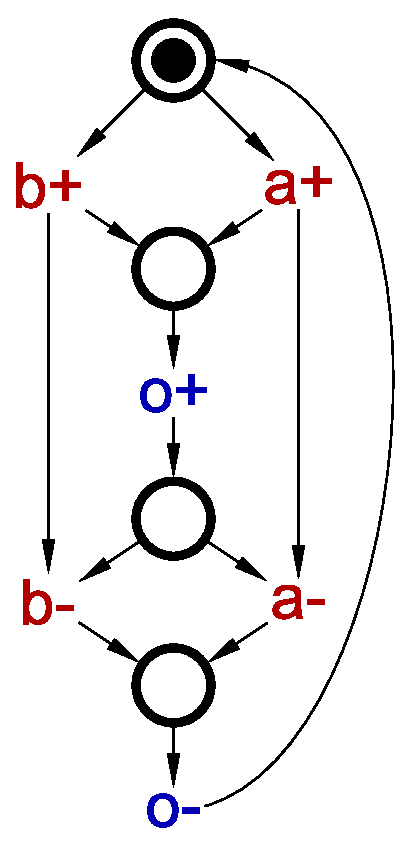
\includegraphics[scale=0.3]{EXPERIMENTS/stg/mix}
        \atop
        \mbox{\rule[1.3em]{0em}{0em}(b) Call}$
        \\[0.5em]
        $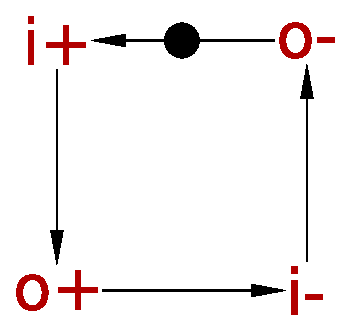
\includegraphics[scale=0.3]{EXPERIMENTS/stg/env}
        \atop
        \mbox{\rule[1.3em]{0em}{0em}(c) Environment}$
    \end{minipage}
    $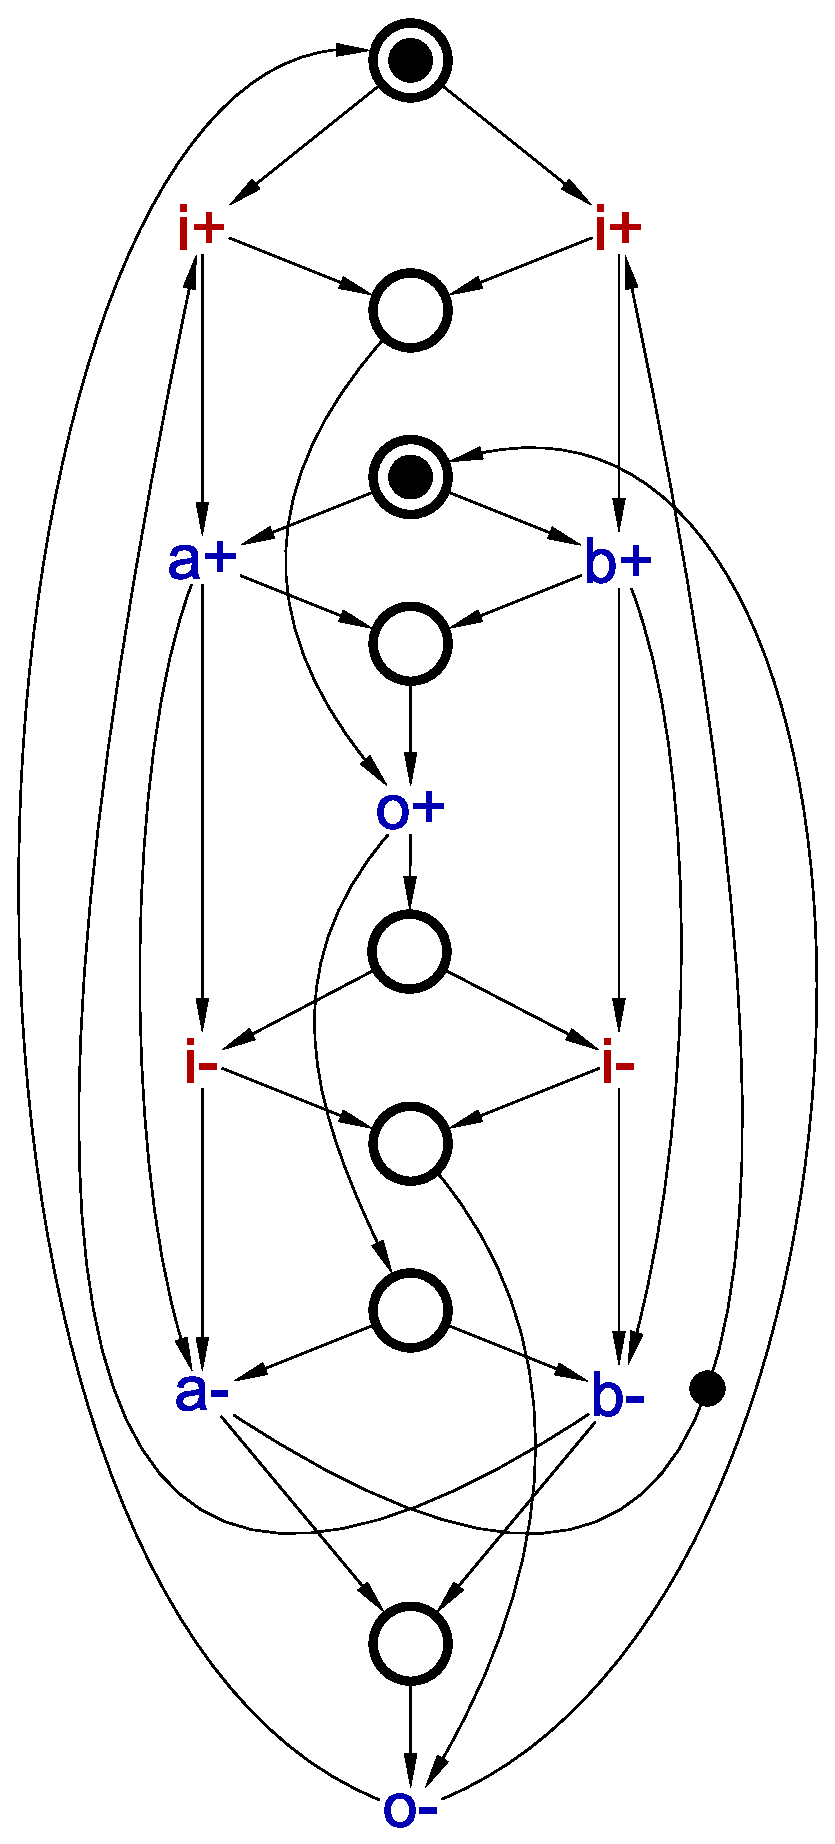
\includegraphics[scale=0.3]{EXPERIMENTS/stg/simple_standard}
    \atop
    \mbox{\rule[1.3em]{0em}{0em}(d) Composition}$
    \caption{\label{fi-motivating-example1}
        Example of standard STG composition.
    }
\end{figure}

\begin{figure}[!tb]
    \centering
    \begin{minipage}[b]{0.4\columnwidth}
        \centering
        $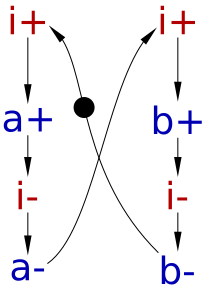
\includegraphics[scale=0.3]{EXPERIMENTS/stg/toggle_opt}
        \atop
        \mbox{\rule[1.3em]{0em}{0em}(a) Toggle}$
        \\[0.5em]
        $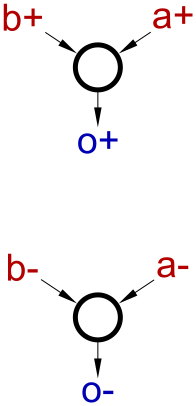
\includegraphics[scale=0.3]{EXPERIMENTS/stg/mix_opt}
        \atop
        \mbox{\rule[1.3em]{0em}{0em}(b) Call}$
        \\[0.5em]
        $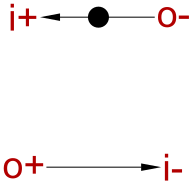
\includegraphics[scale=0.3]{EXPERIMENTS/stg/env_opt}
        \atop
        \mbox{\rule[1.3em]{0em}{0em}(c) Environment}$
    \end{minipage}
    $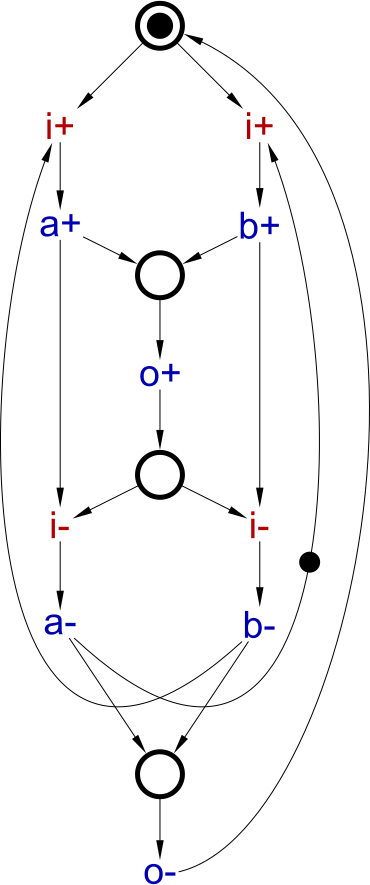
\includegraphics[scale=0.3]{EXPERIMENTS/stg/simple_improved}
    \atop
    \mbox{\rule[1.3em]{0em}{0em}(d) Composition}$
    \caption{\label{fi-motivating-example2}
        Example of improved STG composition: the components are obtained from the corresponding ones in Fig.~\ref{fi-motivating-example1} by removing some places, and then the standard parallel composition is applied to these modified components.
    }
\end{figure}


One operation where implicit places matter is \emph{transition contraction,}~\cite{vowo02lncs} which is a crucial part of the re-syn\-the\-sis approach~\cite{CN-02,KVL-96,PC-96}. The idea is to hide the internal communication between the components (by labelling the corresponding transitions as `dummy' --- they correspond to signals $a$ and $b$ in our example), contract as many of these dummy transitions as possible (whereby reducing the size of the STG), and re-synthesise the obtained STG as a circuit (which is often smaller than the original circuit due to removal of some signals). Transition contraction has to be performed on very large STGs (corresponding to the whole control path of the circuit), and so, for efficiency, it has to be a structural operation. Unfortunately, such structural contractions are not always possible (see Sect.~\ref{sec_pn_basic}), and implicit places in the preset and/or postset of a transition can prevent contracting it, even if a contraction is possible after removing these implicit places. In our example, \desij cannot contract any of the dummy transitions in the STG in Fig.~\ref{fi-motivating-example1}(d), even though it performs some structural tests for place redundancy; however, it is able to contract all the dummy transitions if the implicit places are removed, \ie when applied to the STG in Fig.~\ref{fi-motivating-example2}(d).

The main contribution of this paper is a new me\-thod for computing the parallel composition of labelled Petri nets, that generates fewer implicit places. It uses the \emph{freeness from computation interference (FCI)} assumption, stating that the situation when one component wants to produce an output, but is prevented from doing so by another component which is not ready to receive it, is impossible. Violation of FCI means that the behaviour of the composition does not correspond to that of the physical system. For example, an output of a circuit component cannot be physically disabled by another component that is not ready to receive this signal, and so producing this output will lead to malfunction; however, the composition will be oblivious to it, and behave as if such an output could not be produced.
Hence FCI is a basic correctness requirement --- if it is violated, there is no point in computing parallel composition, as its behaviour will not describe that of the physical system. In practice, FCI is often guaranteed by construction, \eg it is always guaranteed for the control path of a \balsa~\cite{EB-02} or \haste/\tangram~\cite{berkel91,haste-manual} specification of an asynchronous circuit. The idea of using the FCI condition is reminiscent of the method of input/output exposure in the synthesis by direct mapping described in~\cite{SBY-07}, and of the correct by construction composition of Petri nets for circuit components and the environment used in the \ditopn tool~\cite{JF-00}.

The main idea of the method we propose here is illustrated by the example in Fig.~\ref{fi-motivating-example2}. Before doing the parallel composition, one can remove some of the places in the components as shown in parts (a--c) of the figure and then compose the modified STGs. The precise conditions that allow to remove a particular place will be stated in Sect.~\ref{se-main}; at this point it is only important that they are structural and thus can be efficiently checked. This guarantees that the number of places in the resulting Petri net is smaller (as the number of places in the composition is the total number of places in all the components), and, under the FCI assumption, the resulting behaviour will be the same (in the sense of isomorphism of the reachability graphs). In particular, in our example, composing the modified components yields the STG in Fig.~\ref{fi-motivating-example2}(d), which in this case contains no implicit places. Observe that the modified components on their own can have rather bad behaviour and in particular can be non-implementable; however, it does not matter, as they are never used on their own, but only in composition with other components, and the resulting behaviour of the composition is guaranteed to correspond to that of the standard composition.

Re-synthesis of asynchronous circuits is the intended application of the proposed method. However, we envisage that it has a much wider applicability, as composition of labelled Petri nets is a fundamental operation, and the FCI assumption often holds in practice.


We continue the work started in~\cite{2010_mokhov_ieee}
where a formal model, called Conditional Partial Order Graphs (CPOGs),
was introduced. Using CPOGs as a foundation allowed us to represent individual system configurations
and operational modes as annotated graphs and to efficiently overlay them by exploiting
their similarities. However, the CPOG formalism lacks the compositionality
and the ability to compare and transform specifications in a rigorous
manner~\cite{pg_algebra}. In particular, CPOGs always represent a specification as
a `flat' structure, similar to the canonical form defined in Section~\ref{sec:Parametrised-Graphs},
hence a hierarchical representation of a system as a composition of
its components is not possible. We extend this formalism in several
ways:

\begin{itemize}
\item We transition from the graphs representing partial orders to general graphs and lift the assumption of graph acyclicity.
Nevertheless, if a partial orders is the most natural way to represent
a certain aspect of system, this still can be handled. 
\item The new formalism is fully compositional -- it adds algebraic operations for combining existing specifications.
\item We describe the equivalence relation between the specifications as
a set of axioms, obtaining an algebra of parametrised graphs. This set of axioms is proved
to be sound, minimal and complete~\cite{pg_algebra}.
\item We have defined equivalence preserving transformations; this permits one to use the algebra to safely manipulate PG specifications. 
This can be viewed as adding a syntactic level to the semantic representation
of specifications, and is reminiscent of the relationship between digital
circuits and Boolean algebra.
\end{itemize}

Since parametrised graphs are likely to be applied in a safety-critical toolchain, it is imperative to attain a degree of confidence in the properties of the PG formalism. Equally important is to convince prospective users that the technique is sound and lives up to its promises. To fulfil this goal, it was decided to construct in a strict and controlled manner a complete formalisation of the PG formalism. The Agda system \cite{norell:thesis} was chosen for its expressive notation language and extensive support for machine-checked formal inference. Agda has enjoyed a notable success as the basis for the formalisation of wide range of problems in the domain of programming language research~\cite{LTL-types-FRP,indexed-containers}.

%Says that Agda is LCF, what is LCF. What are the altrenatives: Isaballe/HOL, HOL-Light, ACL2, Coq, PVS, Nqthm. What the have achieved (the colouring problem, pentium div, ...)
%
%compare to Maude (2 lines)
%
%a small agda example: list 
%
%explain why an alegbraic specification is better suited than a model-based (VDM, Z, B) or process based (CSP, CCS).
%
%



We demonstrate the usefulness of the developed formalism on the basis of two case
studies. The first one (Section ~\ref{subsect:PhaseEncoders}) is concerned with development of a phase encoding
controller that represents information by the order of arrival of
signals on $n$ wires. As there are $n!$ possible arrival orders,
it is a challenge to specify the set of corresponding behavioural
scenarios in a compact way. The proposed formalism not only allows us
to solve this problem but also does it in a compositional manner. The final specification is obtained through the composition of fixed-size fragments
describing the behaviours of a pair of wires (the latter is impossible
with the CPOG formalism).


%{\huge TODO}
%The second case study (Section ~\ref{subsect:MicrocontrollerDesign}) is concerned with designing a microcontroller
%for a simple processor. The processor can execute several classes
%of instructions and each class is characterised by a specific execution
%scenario of the operational units of the processor. In turn, the scenarios
%of conditional instructions have to be composed of sub-scenarios corresponding
%to the current value of the appropriate ALU flag. The overall specification
%of the microcontroller is then obtained algebraically by composing
%scenarios of each class of instructions.




\section{Conditional Partial Order Graphs\label{sec:CPOG-model-essentials}}

A \emph{Conditional Partial Order Graph}~\cite{2009_mokhov_phd}\cite{2010_mokhov_ieee}
is a quintuple $H=(V,\ E,\ X,\ \rho,\ \phi)$, where $V$ is a finite
set of \emph{vertices}, $E\subseteq V\times V$ is a set of \emph{arcs}
between them, and $X$ is a finite set of \emph{operational}\emph{variables}. An \emph{opcode} is an assignment $(x_{1},\ x_{2},\ \dots,\ x_{|X|})\in\{0,\ 1\}^{|X|}$
of these variables; $X$ can be assigned only those opcodes which
satisfy the \emph{restriction function} $\rho$
of the graph, i.e. $\rho(x_{1},\ x_{2},\ \dots,\ x_{|X|})=1$. Function
$\phi$ assigns a Boolean \emph{condition} $\phi(z)$ to every vertex
and arc $z\in V\cup E$ of the graph.

\begin{figure}[h]
\hfill{}\subfloat[Full notation]{

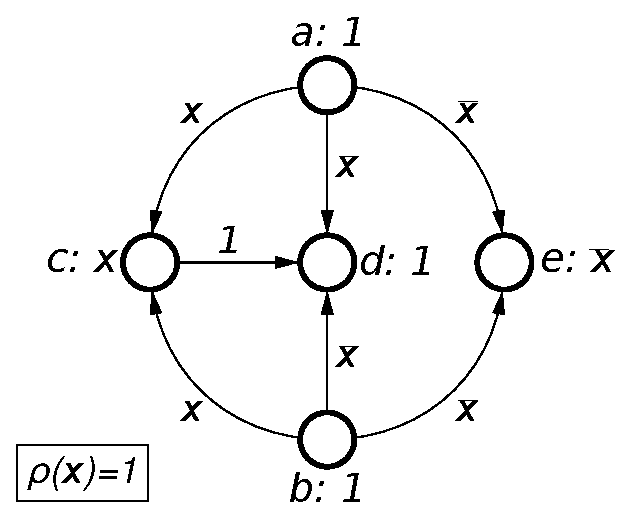
\includegraphics[scale=0.45]{fig/cpog}}\hfill{}\subfloat[Simplified notation]{

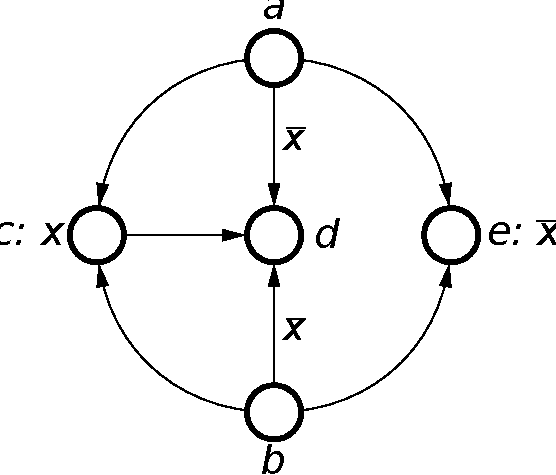
\includegraphics[scale=0.45]{fig/cpog_simplified}}\hfill{}

\begin{centering}
\subfloat[Multiple CPOG projections]{\begin{centering}
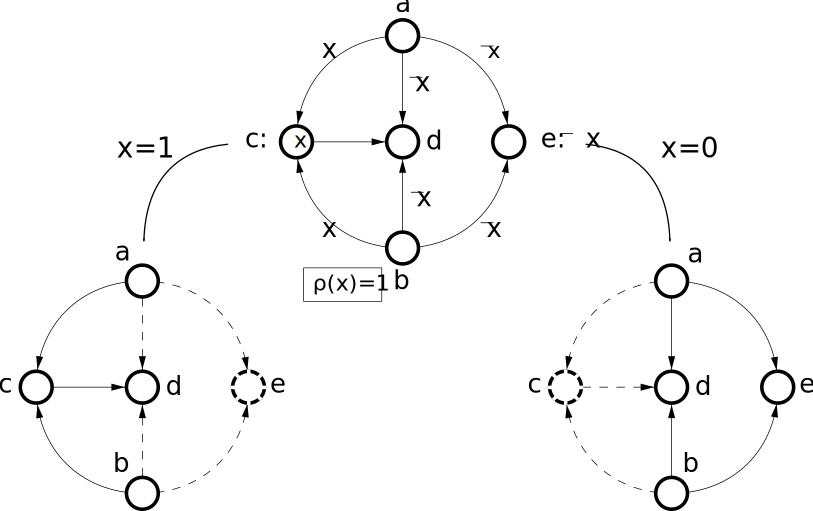
\includegraphics[scale=0.45]{fig/cpog_projections_2}
\par\end{centering}

}
\par\end{centering}

\caption{\label{fig-cpog-examples}Graphical representation of CPOGs and their projections}
\end{figure}


Figure~\ref{fig-cpog-examples}(a) shows an example of a CPOG containing
$|V|=5$ vertices and $|E|=7$ arcs. There is a single operational
variable $x$; the restriction function is $\rho(x)=1$, hence both
opcodes $x=0$ and $x=1$ are allowed. Vertices $\{a,\ b,\ d\}$ have
constant $\phi=1$ conditions and are called \emph{unconditional},
while vertices $\{c,\ e\}$ are \emph{conditional} and have conditions
$\phi(c)=x$ and $\phi(e)=\overline{x}$ respectively. Arcs also fall
into two classes: unconditional (arc $c\rightarrow d$) and conditional
(all the rest). As CPOGs tend to have many unconditional vertices
and arcs we use a simplified notation in which conditions equal to
$1$ are not depicted in the graph. This is demonstrated in Figure~\ref{fig-cpog-examples}(b).

The purpose of conditions $\phi$ is to `switch off' some vertices
and/or arcs in the graph according to the given opcode. This makes
CPOGs capable of specifying multiple partial orders or instructions
(a partial order is a form of behavioural description of an instruction).
Figure~\ref{fig-cpog-examples}(c) shows a graph and its two \emph{projections}.
The leftmost projection is obtained by keeping in the graph only those
vertices and arcs whose conditions evaluate to $1$ after substitution
of the operational variable $x$ with $1$. Hence, vertex $e$ disappears,
because its condition evaluates to $0$: $\phi(e)=\overline{x}=\overline{1}=0$.
Arcs $\{a\rightarrow d,\ a\rightarrow e,\ b\rightarrow d,\ b\rightarrow e\}$
disappear for the same reason. The rightmost projection is obtained
in the same way with the only difference that variable $x$ is set
to $0$. Note also that although the condition of arc $c\rightarrow d$
evaluates to $1$ (in fact it is constant $1$) the arc is still excluded
from the resultant graph because one of the vertices it connects (vertex
$c$) is excluded and obviously an arc cannot appear in a graph without
one of its vertices. Each of the obtained projections can be treated
as a specification of a particular behavioural scenario of the modelled
system. Potentially, a CPOG $H=(V,\ E,\ X,\ \rho,\ \phi)$ can specify
an exponential number of different partial orders of events in $V$
according to one of $2^{|X|}$ different possible opcodes.

A CPOG is \emph{well-defined} if all its projections allowed by
$\rho$ are acyclic. We consider only well-defined CPOGs in this thesis,
because a cyclic projection has no natural execution semantics, in
particular it is not clear which event can be executed first unless
some form of a \textquoteleft{}token\textquoteright{} is introduced
as in the Petri Net model~\cite{2002_cortadella_book}.

To summarise, a CPOG is a structure to represent a set of encoded
partial orders in a compact form. Synthesis and optimisation methods
presented in~\cite{2010_mokhov_ieee} provide a way to obtain such
a representation given a set of partial orders and their opcodes.
For example, the CPOG in Figure~\ref{fig-cpog-examples}(c) can be
synthesised automatically from the two partial orders below it and
the corresponding opcodes $x=1$ and $x=0$. The next section shows
that a particular assignment of opcodes to the partial orders has
a strong impact on the final CPOG, therefore in order to obtain the
most compact CPOG representation one has to search for the best opcode
assignment.

Note that partial orders is not the only formalism for formal specification
of instructions. In particular, there is an alternative approach~\cite{1994_baranov_book}
based on automata, which treats every instruction as a burst-mode
state machine and defines an operation of composition on them. While
benefiting from a direct correspondence between flowcharts of algorithms
and automata, the approach cannot model true concurrency: a set of
causally independent events can only be executed as a `burst' in
the same step/clock cycle. Also, it requires explicit memory to track
the current state of the automaton. We believe that partial orders
are better suited for modelling instruction sets of processing units
built on heterogeneous platforms, i.e. exhibiting both asynchronous
and synchronous interactions~\cite{2011_mokhov_tr}.


%include lhs2TeX.fmt
%include polycode.fmt

\usepackage{amstext}
\usepackage{amssymb}
\usepackage{stmaryrd}

\DeclareMathAlphabet{\mathkw}{OT1}{cmss}{bx}{n}

\newcommand{\redFG}[1]{\textcolor[rgb]{0.6,0,0}{#1}}
\newcommand{\greenFG}[1]{\textcolor[rgb]{0,0.4,0}{#1}}
\newcommand{\blueFG}[1]{\textcolor[rgb]{0,0,0.8}{#1}}
\newcommand{\orangeFG}[1]{\textcolor[rgb]{0.8,0.4,0}{#1}}
\newcommand{\purpleFG}[1]{\textcolor[rgb]{0.4,0,0.4}{#1}}
\newcommand{\yellowFG}[1]{\textcolor{yellow}{#1}}
\newcommand{\brownFG}[1]{\textcolor[rgb]{0.5,0.2,0.2}{#1}}
\newcommand{\blackFG}[1]{\textcolor[rgb]{0,0,0}{#1}}
\newcommand{\whiteFG}[1]{\textcolor[rgb]{1,1,1}{#1}}
\newcommand{\yellowBG}[1]{\colorbox[rgb]{1,1,0.2}{#1}}
\newcommand{\brownBG}[1]{\colorbox[rgb]{1.0,0.7,0.4}{#1}}

\newcommand{\ColourStuff}{
  \newcommand{\red}{\redFG}
  \newcommand{\green}{\greenFG}
  \newcommand{\blue}{\blueFG}
  \newcommand{\orange}{\orangeFG}
  \newcommand{\purple}{\purpleFG}
  \newcommand{\yellow}{\yellowFG}
  \newcommand{\brown}{\brownFG}
  \newcommand{\black}{\blackFG}
  \newcommand{\white}{\whiteFG}
}

\newcommand{\MonochromeStuff}{
  \newcommand{\red}{\blackFG}
  \newcommand{\green}{\blackFG}
  \newcommand{\blue}{\blackFG}
  \newcommand{\orange}{\blackFG}
  \newcommand{\purple}{\blackFG}
  \newcommand{\yellow}{\blackFG}
  \newcommand{\brown}{\blackFG}
  \newcommand{\black}{\blackFG}
  \newcommand{\white}{\blackFG}
}

\ColourStuff

\newcommand{\K}[1]{\yellow{\mathsf{#1}}}
\newcommand{\Q}[1]{\green{\mathsf{#1}}}
\newcommand{\D}[1]{\blue{\mathsf{#1}}}
\newcommand{\C}[1]{\red{\mathsf{#1}}}
\newcommand{\F}[1]{\green{\mathsf{#1}}}
\newcommand{\V}[1]{\purple{\mathit{#1}}}

\newcommand{\dfeq}{\overset{\mathrm{df}}{=}}

%%%%%%% BREAK HERE %%%%%%%

\chapter{Algebra of Parameterised Graphs}

\label{chap:PGAlgebra}

\section{Parameterised Graphs\label{sec:Parametrised-Graphs}}

A \emph{Parameterised Graph} (PG) is a model which has evolved from
Conditional Partial Order Graphs (CPOG)~\cite{2010_mokhov_ieee}.
We consider directed graphs $G=(V,E)$ whose vertices are picked from
the fixed alphabet of \emph{actions} $\mathcal{A}=\{a,b,...\}$. Hence
the vertices of $G$ would usually model actions (or \emph{events})
of the system being designed, while the arcs would usually model the
\emph{precedence} or \emph{causality} relation: if there is an arc
going from~$a$ to~$b$ then action~$a$ precedes action~$b$.
We will denote the \emph{empty graph} $(\emptyset,\emptyset)$ by
$\varepsilon$ and the \emph{singleton graphs} $(\{a\},\emptyset)$
simply by $a$, for any $a\in\mathcal{A}$.

Let $G_{1}=(V_{1},E_{1})$ and $G_{2}=(V_{2},E_{2})$ be two graphs,
where $V_{1}$ and $V_{2}$ as well as $E_{1}$ and $E_{2}$ are not
necessarily disjoint. We define the following operations on graphs
(in the order of increasing precedence):
\begin{lyxlist}{00.00.0000}
\item [{\hspace{6mm}Overlay:}] $G_{1}+G_{2}\dfeq(V_{1}\cup V_{2},E_{1}\cup E_{2})$.
\item [{\hspace{6mm}Sequence:}] $G_{1}\rightarrow G_{2}\dfeq(V_{1}\cup V_{2},E_{1}\cup E_{2}\cup V_{1}\times V_{2})$.
\item [{\hspace{6mm}Condition:}] $[1]G\dfeq G$ and
$[0]G\dfeq\varepsilon$.
\end{lyxlist}
In other words, the \emph{overlay}~$+$ and \emph{sequence}~$\rightarrow$
are binary operations on graphs with the following semantics: $G_{1}+G_{2}$
is a graph obtained by \emph{overlaying} graphs~$G_{1}$ and~$G_{2}$,
i.e. it contains the union of their vertices and arcs, while graph
$G_{1}\rightarrow G_{2}$ contains the union plus the arcs connecting
every vertex from graph~$G_{1}$ to every vertex from graph~$G_{2}$
(self-loops can be formed in this way if $V_{1}$ and $V_{2}$ are
not disjoint). From the behavioural point of view, if graphs~$G_{1}$
and~$G_{2}$ correspond to two systems then $G_{1}+G_{2}$ corresponds
to their \emph{parallel composition} and $G_{1}\rightarrow G_{2}$
corresponds to their \emph{sequential composition}. One can observe
that any non-empty graph can be obtained by successively applying
the operations $+$ and $\rightarrow$ to the singleton graphs.

Fig.~\ref{fig:Overlay-and-sequence-no-common} shows an example of
two graphs together with their overlay and sequence. One can see that
the overlay does not introduce any dependencies between the actions
coming from different graphs, therefore they can be executed concurrently.
On the other hand, the sequence operation imposes the order on the
actions by introducing new dependencies between actions $a$, $b$
and $c$ coming from graph $G_{1}$ and action $d$ coming from graph
$G_{2}$. Hence, the resulting system behaviour is interpreted as
the behaviour specified by graph $G_{1}$ followed by the behaviour
specified by graph $G_{2}$. Another example of system composition
is shown in Fig.~\ref{fig:Overlay-and-sequence}. Since the graphs
have common vertices, their compositions are more complicated, in
particular, their sequence contains the self-dependencies $(b,b)$
and $(d,d)$ which lead to a \emph{deadlock} in the resulting system:
action~$a$ can occur, but all the remaining actions are locked.

Given a graph~$G$, the unary \emph{condition} operations can either
preserve it (\emph{true condition} $[1]G$) or nullify it (\emph{false
condition} $[0]G$). They should be considered as a family $\{[b]\}_{b\in\mathbb{B}}$
of operations parameterised by a Boolean value~$b$.

Having defined the basic operations on the graphs, one can build graph
expressions using these operations, the empty graph $\varepsilon$,
the singleton graphs $a\in\mathcal{A}$, and the Boolean constants
$0$ and $1$ (as the parameters of the conditional operations) ---
much like the usual arithmetical expressions. We now consider replacing
the Boolean constants with Boolean variables or general predicates
(this step is akin going from arithmetic to algebraic expressions).
The value of such an expression depends on the values of its parameters,
and so we call such an expression a \emph{parameterised graph}~(PG).

One can easily prove the following properties of the operations introduced
above.
\begin{itemize}
\item \hspace{-1mm}Properties of overlay:

\begin{lyxlist}{00.00.0000}
\item [{\hspace{2mm}Identity:}] $G+\varepsilon=G$
\item [{\hspace{2mm}Commutativity:}] $G_{1}+G_{2}=G_{2}+G_{1}$
\item [{\hspace{2mm}Associativity:}] $(G_{1}+G_{2})+G_{3}=G_{1}+(G_{2}+G_{3})$
\end{lyxlist}
\item \hspace{-1mm}Properties of sequence:

\begin{lyxlist}{00.00.0000}
\item [{\hspace{2mm}Left~identity:}] $\varepsilon\rightarrow G=G$
\item [{\hspace{2mm}Right~identity:}] $G\rightarrow\varepsilon=G$
\item [{\hspace{2mm}Associativity:}] $(G_{1}\!\rightarrow\! G_{2})\!\rightarrow\! G_{3}=G_{1}\!\rightarrow\!(G_{2}\!\rightarrow\! G_{3})$
\end{lyxlist}
\item \hspace{-1mm}Other properties:


\hspace{2mm}Left/right~distributivity: \vspace{-0.3em}
\[
\begin{array}{c}
G_{1}\rightarrow(G_{2}+G_{3})=G_{1}\rightarrow G_{2}+G_{1}\rightarrow G_{3}\\
(G_{1}+G_{2})\rightarrow G_{3}=G_{1}\rightarrow G_{3}+G_{2}\rightarrow G_{3}
\end{array}
\]
\vspace{-1em}


\hspace{2mm}Decomposition: \vspace{-0.3em}
\[
G_{1}\!\rightarrow\! G_{2}\!\rightarrow\! G_{3}\!=\! G_{1}\!\rightarrow\! G_{2}+G_{1}\!\rightarrow\! G_{3}+G_{2}\!\rightarrow\! G_{3}
\]
\vspace{-1.3em}


\item \hspace{-1mm}Properties involving conditions:

\begin{lyxlist}{00.00.0000}
\item [{\hspace{2mm}Conditional~$\varepsilon$:}] $[b]\varepsilon=\varepsilon$
\item [{\hspace{2mm}Conditional~overlay:}] $[b](G_{1}+G_{2})=[b]G_{1}+[b]G_{2}$
\item [{\hspace{2mm}Conditional~sequence:}] \hspace{-0.5mm}$[b](G_{1}\!\rightarrow\! G_{2})\!=\![b]G_{1}\!\rightarrow\![b]G_{2}$
\item [{\hspace{2mm}AND-condition:}] $[b_{1}\wedge b_{2}]G=[b_{1}][b_{2}]G$
\item [{\hspace{2mm}OR-condition:}] $[b_{1}\vee b_{2}]G=[b_{1}]G+[b_{2}]G$
\end{lyxlist}

\hspace{2mm}Condition~regularisation: \vspace{-0.3em}
\[
[b_{1}]G_{1}\!\rightarrow\![b_{2}]G_{2}\!=\![b_{1}]G_{1}+[b_{2}]G_{2}+[b_{1}\wedge b_{2}](G_{1}\!\rightarrow\! G_{2})
\]


\end{itemize}
Now, due to the above properties of the operators, it is possible
to define the following canonical form of a PG. In the proof below,
we call a singleton graph, possibly prefixed with a condition, a \emph{literal}.
\begin{prop}
[Canonical form of a PG]\label{prop:Canonical-form} Any PG can be
rewritten in the following canonical form:
\begin{equation}
\left(\sum_{v\in V}[b_{v}]v\right)+\left(\sum_{u,v\in V}[b_{uv}](u\rightarrow v)\right),\label{eq:canonical-form}
\end{equation}


where:
\begin{itemize}
\item $V$ is a subset of singleton graphs that appear in the original PG;
\item for all $v\in V$, $b_{v}$ are canonical forms of Boolean expressions
and are distinct from 0;
\item for all $u,v\in V$, $b_{uv}$ are canonical forms of Boolean expressions
such that $b_{uv}\Rightarrow b_{u}\wedge b_{v}$.
\end{itemize}
\end{prop}
\begin{proof}
(i) First we prove that any PG can be converted to the form~(\ref{eq:canonical-form}).

All the occurrences of $\varepsilon$ in the expression can be eliminated
by the identity and conditional $\varepsilon$ properties (unless
the whole PG equals to $\varepsilon$, in which case we take $V=\emptyset$).
To avoid unconditional subexpressions, we prefix the resulting expression
with `$[1]$', and then by the conditional overlay/sequence properties
we propagate all the conditions that appear in the expression down
to the singleton graphs (compound conditions can be always reduced
to a single one by the AND-condition property). By the decomposition
and distributivity properties, the expression can be rewritten as
an overlay of literals and subexpressions of the form $l_{1}\rightarrow l_{2}$,
where $l_{1}$ and $l_{2}$ are literals. The latter subexpressions
can be rewritten using the condition regularisation rule:
\[
[b_{1}]u\rightarrow[b_{2}]v=[b_{1}]u+[b_{2}]v+[b_{1}\wedge b_{2}](u\rightarrow v)
\]
Now, literals corresponding to the same singleton graphs, as well
as subexpressions of the form $[b](u\rightarrow v)$ that correspond
to the same pair of singleton graphs $u$ and $v$, are combined using
the OR-condition property. Then the literals prefixed with 0 conditions
can be dropped. Now the set $V$ consists of all the singleton graphs
occurring in the literals. To turn the overall expression into the
required form it only remains to add missing subexpressions of the
form $[0](u\rightarrow v)$ for every $u,v\in V$ such that the expression
does not contain the subexpression of the form $[b](u\rightarrow v)$.
Note that the property $b_{uv}\Rightarrow b_{u}\wedge b_{v}$ is always
enforced by this construction:
\begin{itemize}
\item condition regularisation ensures this property;
\item combining literals using the OR-condition property can only strengthen
the right hand side of this implication, and so cannot violate it;
\item adding $[0](u\rightarrow v)$ does not violate the property as it
trivially holds when $b_{uv}=0$.
\end{itemize}
(ii) We now show that (\ref{eq:canonical-form}) is a canonical form,
i.e. if $L=R$ then their canonical forms $\mathit{can}(L)$ and $\mathit{can}(R)$
coincide.

For the sake of contradiction, assume this is not the case. Then we
consider two cases (all possible cases are symmetric to one of these
two):
\begin{enumerate}
\item $\mathit{can}(L)$ contains a literal $[b_{v}]v$ whereas $\mathit{can}(R)$
either contains a literal $[b_{v}']v$ with $b_{v}'\not\equiv b_{v}$
or does not contain any literal corresponding to $v$, in which case
we say that it contains a literal $[b_{v}']v$ with $b_{v}'=0$. Then
for some values of parameters one of the graphs will contain vertex
$v$ while the other will not.
\item $\mathit{can}(L)$ and $\mathit{can}(R)$ have the same set $V$ of
vertices, but $\mathit{can}(L)$ contains a subexpression \foreignlanguage{english}{$[b_{uv}](u\rightarrow v)$}
whereas $\mathit{can}(R)$ contains a subexpression \foreignlanguage{english}{$[b_{uv}'](u\rightarrow v)$}
with $b_{uv}'\not\equiv b_{uv}$. Then for some values of parameters
one of the graphs will contain the arc $(u,v)$ (note that due to
$b_{uv}\Rightarrow b_{u}\wedge b_{v}$ and $b_{uv}'\Rightarrow b_{u}\wedge b_{v}$
vertices $u$ and $v$ are present), while the other will not.
\end{enumerate}
In both cases there is a contradiction with $L=R$.
\end{proof}
This canonical form allows one to lift the notion of \emph{adjacency
matrix} of a graph to PGs. Recall that the adjacency matrix $(b_{uv})$
of a graph $(V,E)$ is a $||V||\times||V||$ Boolean matrix such that
$b_{uv}=1$ if $(u,v)\in E$ and $b_{uv}=0$ otherwise. The adjacency
matrix of a PG is obtained from the canonical form~(\ref{eq:canonical-form})
by gathering the predicates $b_{uv}$ into a matrix. The adjacency
matrix of a PG is similar to that of a graph, but it contains predicates
rather than Boolean values. It does not uniquely determine a PG, as
the predicates of the vertices cannot be derived from it; to fully
specify a PG one also has to provide predicates $b_{v}$ from the
canonical form~(\ref{eq:canonical-form}). 

Another advantage of this canonical form is that it provides a graphical
notation for PGs. The vertices occurring in the canonical form (set
$V$) can be represented by circles, and the subexpressions of the
form $u\rightarrow v$ by arcs. The label of a vertex $v$ consists
of the vertex name, colon and the predicate $b_{v}$, while every
arc~$(u,v)$ is labelled with the corresponding predicate $b_{uv}$.
As adjacency matrices of PGs tend to have many constant elements,
we use a simplified notation in which the arcs with constant~0 predicates
are not drawn, and constant~1 predicates are dropped; moreover, it
is convenient to assume that the predicates on arcs are implicitly
ANDed with those on incident vertices (to enforce the invariant $b_{uv}\Rightarrow b_{u}\wedge b_{v}$),
which often allows one to simplify predicates on arcs. This can be
justified by introducing the ternary operator, called \emph{conditional
sequence}:
\[
u\overset{b}{\longrightarrow}v\overset{\text{df}}{=}[b](u\rightarrow v)+u+v
\]
Intuitively, PG $u\overset{b}{\longrightarrow}v$ consists of two
unconditional vertices connected by an arc with the condition $b$.
By case analysis on $b_{1}$ and $b_{2}$ one can easily prove the
following properties of the conditional sequence that allow simplifying
the predicates on arcs:
\begin{eqnarray*}
[b_{1}]u\xrightarrow{b_{1}\wedge b_{2}}v & = & [b_{1}]u\overset{b_{2}}{\longrightarrow}v\\
u\xrightarrow{b_{1}\wedge b_{2}}[b_{2}]v & = & u\overset{b_{1}}{\longrightarrow}[b_{2}]v
\end{eqnarray*}


Fig.~\ref{fig:Specialisations}(top) shows an example of a PG. The
predicates depend on a Boolean variable~$x$. The predicates of vertices~$a$,
$b$ and $d$ are constants~$1$; such vertices are called \emph{unconditional}.
Vertices~$c$ and~$e$ are \emph{conditional,} and their predicates
are $x$ and $\overline{x}$, respectively. Arcs also fall into two
classes: \emph{unconditional,} i.e. those whose predicate and the
predicates of their incident vertices are constants~1, and \emph{conditional}
(in this example, all the arcs are conditional).

A \emph{specialisation $H\vert_{p}$ of a PG $H$ under predicate
$p$} is a PG, whose predicates are simplified under the assumption
that $p$ holds. If $H$ specifies the behaviour of the whole system,
$H\vert_{p}$ specifies the part of the behaviour that can be realised
under condition $p$. An example of a graph and its two specialisations
is presented in Fig.~\ref{fig:Specialisations}. The leftmost specialisation
$H\vert_{x}$ is obtained by removing from the graph those vertices
and arcs whose predicates evaluate to~0 under condition~$x$, and
simplifying the other predicates. Hence, vertex~$e$ and arcs $(a,d)$,
$(a,e)$, $(b,d)$ and $(b,e)$ disappear, and all the other vertices
and arcs become unconditional. The rightmost specialisation $H\vert_{\overline{x}}$
is obtained analogously. Each of the obtained specialisations can
be regarded as a specification of a particular behavioural scenario
of the modelled system, e.g. as specification of a processor instruction.

\begin{figure}
\begin{centering}
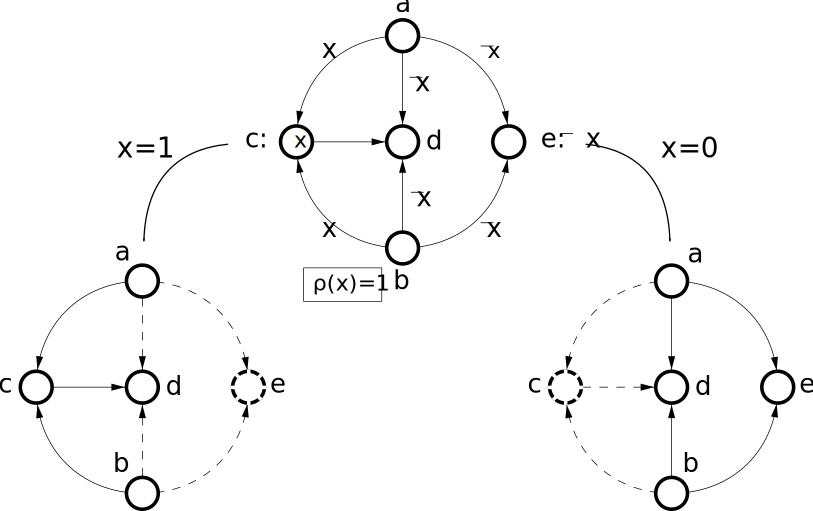
\includegraphics[width=1\columnwidth]{fig/cpog_projections_2}
\par\end{centering}

\caption{\label{fig:Specialisations}PG specialisations: $H\vert_{x}$ and
$H\vert_{\overline{x}}$}
\end{figure}



\subsection{Specification and composition of instructions}

Consider a processing unit that has two registers $A$ and $B$, and
can perform two different instructions: \emph{addition} and \emph{exchange}
of two variables stored in memory. The processor contains five datapath
components (denoted by $a\dots e$) that can perform the following
atomic actions:\renewcommand{\labelenumi}{\alph{enumi})}
\begin{enumerate}
\item Load register $A$ from memory;
\item Load register $B$ from memory;
\item Compute the sum of the numbers stored in registers~$A$ and~$B$,
and store it in $A$;
\item Save register $A$ into memory;
\item Save register $B$ into memory.
\end{enumerate}
\renewcommand{\labelenumi}{\arabic{enumi}.}Table~\ref{tab-two-operations}
describes the addition and exchange instructions in terms of usage
of these atomic actions.

The addition instruction consists of loading the two operands from
memory (causally independent actions~$a$ and~$b$), their addition
(action~$c$), and saving the result (action~$d$). Let us assume
for simplicity that in this example all causally independent actions
are always performed concurrently, see the corresponding scenario
$\mathit{ADD}$ in the table.

\begin{table}
\begin{centering}
\begin{tabular}{||c||||c||||c||c||}
\hline 
\multicolumn{2}{||c||||}{Instruction} & Addition & Exchange\tabularnewline
\hline 
\multicolumn{2}{||c||||}{} & \multicolumn{1}{l||}{~a) Load $A$} & \multicolumn{1}{l||}{~a) Load $A$}\tabularnewline
\multicolumn{2}{||c||||}{Action} & \multicolumn{1}{l||}{~b) Load $B$} & \multicolumn{1}{l||}{~b) Load $B$}\tabularnewline
\multicolumn{2}{||c||||}{sequence} & \multicolumn{1}{l||}{~c) Add $B$ to $A$} & \multicolumn{1}{l||}{~d) Save $A$}\tabularnewline
\multicolumn{2}{||c||||}{} & \multicolumn{1}{l||}{~d) Save $A$} & \multicolumn{1}{l||}{~e) Save $B$}\tabularnewline
\hline 
\multicolumn{2}{||c||||}{Execution} & 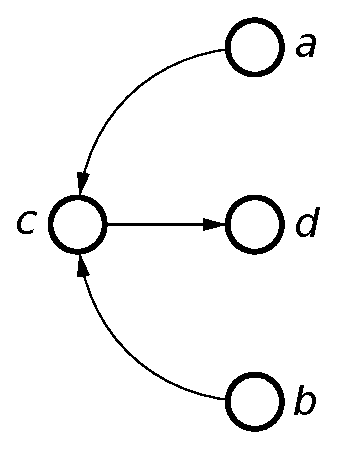
\includegraphics[bb=-10bp 90bp 158bp 220bp,scale=0.4]{fig/projection_1}~~~ & 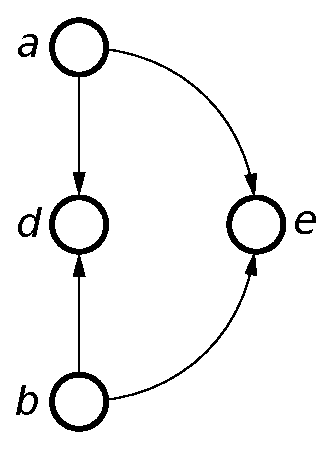
\includegraphics[bb=-20bp 90bp 157bp 220bp,scale=0.4]{fig/projection_2}\tabularnewline
\multicolumn{2}{||c||||}{scenario} &  & \tabularnewline
\multicolumn{2}{||c||||}{with maximum} &  & \tabularnewline
\multicolumn{2}{||c||||}{concurrency} &  & \tabularnewline
\multicolumn{2}{||c||||}{} &  & \tabularnewline
\multicolumn{2}{||c||||}{} &  & \tabularnewline
\multicolumn{2}{||c||||}{} & $\mathit{ADD}$ & $\mathit{XCHG}$\tabularnewline
\multicolumn{2}{||c||||}{} &  & \tabularnewline
\hline 
\end{tabular}
\par\end{centering}

\caption{\label{tab-two-operations}Two instructions specified as partial orders}
\end{table}


The operation of exchange consists of loading the operands (causally
independent actions~$a$ and~$b$), and saving them into swapped
memory locations (causally independent actions $d$ and $e$), as
captured by the $\mathit{XCHG}$ scenario. Note that in order to start
saving one of the registers it is necessary to wait until both of
them have been loaded to avoid overwriting one of the values.

One can see that the two scenarios in Table~\ref{tab-two-operations}
appear to be the two specialisations of the PG shown in Fig.~\ref{fig:Specialisations},
thus this PG can be considered as a joint specification of both instructions.
Two important characteristics of such a specification are that the
common events $\{a,b,d\}$ are overlaid, and the choice between the
two operations is modelled by the Boolean predicates associated with
the vertices and arcs of the PG. As a result, in our model there is
no need for a `nodal point' of choice, which tend to appear in alternative
specification models: a Petri Net (resp. Finite State Machine) would
have an explicit choice place (resp. state), and a specification written
in a Hardware Description Language would describe the two instructions
by two separate branches of a conditional statement~\texttt{if} or~\texttt{case}~\cite{1994_de_micheli_book}).

The PG operations introduced above allow for a natural specification
of the system as a collection of its behavioural scenarios, which
can share some common parts. For example, in this case the overall
system is composed as
\begin{equation}
\begin{array}{c}
H=[x]ADD+[\overline{x}]XCHG=\\
=\![x]((a\!+\! b)\!\rightarrow\! c\!+\! c\!\rightarrow\! d)\!+\![\overline{x}]((a\!+\! b)\!\rightarrow\!(d\!+\! e)).
\end{array}\label{eq:H_ADD_XCHG}
\end{equation}
Such specifications can often be simplified using the properties of
graph operations. The next section describes the equivalence relation
between the PGs with a set of axioms, thus obtaining an algebra.


\section{Algebra of parameterised graphs\label{sec:Algebra-of-parametrised}}

In this section we define the \emph{algebra of parameterised graphs}
(PG-algebra).

PG-algebra is a tuple~$\left\langle \mathcal{G},+,\rightarrow,[0],[1]\right\rangle $,
where~$\mathcal{G}$ is a set of graphs whose vertices are picked
from the alphabet~$\mathcal{A}$ and the operations parallel those
defined for graphs above. The equivalence relation is given by the
following axioms.
\begin{itemize}
\item $+$ is commutative and associative
\item $\rightarrow$ is associative
\item $\varepsilon$ is a left and right identity of $\rightarrow$
\item $\rightarrow$ distributes over $+$:\vspace{-0.3em}
\[
\begin{array}{c}
p\rightarrow(q+r)=p\rightarrow q+p\rightarrow r\\
(p+q)\rightarrow r=p\rightarrow r+q\rightarrow r
\end{array}
\]

\item Decomposition: \vspace{-0.3em}
\[
p\rightarrow q\rightarrow r=p\rightarrow q+p\rightarrow r+q\rightarrow r
\]

\item Condition: $[0]p=\varepsilon$ and $[1]p=p$
\end{itemize}
The following derived equalities can be proved from PG-algebra axioms~\cite[Prop. 2, 3]{2011_mokhov_pg}:
\begin{itemize}
\item $\varepsilon$ is an identity of $+$: $p+\varepsilon=p$
\item $+$ is idempotent: $p+p=p$
\item Left and right absorption:\vspace{-0.3em}
\[
\begin{array}{c}
p+p\rightarrow q=p\rightarrow q\\
q+p\rightarrow q=p\rightarrow q
\end{array}
\]

\item Conditional $\varepsilon$: $[b]\varepsilon=\varepsilon$
\item Conditional overlay: $[b](p+q)=[b]p+[b]q$
\item Conditional sequence: $[b](p\rightarrow q)=[b]p\rightarrow[b]q$
\item AND-condition: $[b_{1}\wedge b_{2}]p=[b_{1}][b_{2}]p$
\item OR-condition: $[b_{1}\vee b_{2}]p=[b_{1}]p+[b_{2}]p$
\item Choice propagation:\vspace{-0.3em}
\[
\begin{array}{c}
[b](p\rightarrow q)+[\overline{b}](p\rightarrow r)=p\rightarrow([b]q+[\overline{b}]r)\\
{}[b](p\rightarrow r)+[\overline{b}](q\rightarrow r)=([b]p+[\overline{b}]q)\rightarrow r
\end{array}
\]

\item Condition regularisation:\vspace{-0.3em}
\[
[b_{1}]p\rightarrow[b_{2}]q=[b_{1}]p+[b_{2}]q+[b_{1}\wedge b_{2}](p\rightarrow q)
\]

\end{itemize}
Note that as $\varepsilon$ is a left and right identity of $\rightarrow$
and $+$, there can be no other identities for these operations. Interestingly,
unlike many other algebras, the two main operations in the PG-algebra
have the same identity.

It is easy to see that PGs are a model of PG-algebra, as all the axioms
of PG-algebra are satisfied by PGs; in particular, this means that
PG-algebra is \emph{sound}. Moreover, any PG-algebra expression has
the canonical form~(\ref{eq:canonical-form}), as the proof of Prop.~\ref{prop:Canonical-form}
can be directly imported: 
\begin{itemize}
\item It is always possible to translate a PG-algebra expression to this
canonical form, as part~(i) of the proof relies only on the properties
of PGs that correspond to either PG-algebra axioms or equalities above.
\item If $L=R$ holds in PG-algebra then $L=R$ holds also for PGs (as PGs
are a model of PG-algebra), and so the PGs $\mathit{can}(L)$ and
$\mathit{can}(R)$ coincide, see part~(ii) of the proof. Since PGs
$\mathit{can}(L)$ and $\mathit{can}(R)$ are in fact the same objects
as the expressions $\mathit{can}(L)$ and $\mathit{can}(R)$ of the
PG-algebra, (\ref{eq:canonical-form}) is a canonical form of a PG-algebra
expression.
\end{itemize}
This also means that PG-algebra is \emph{complete} w.r.t. PGs, i.e.
any PG equality can be either proved or disproved using the axioms
of PG-algebra (by converting to the canonical form). 

The provided set of axioms of PG-algebra is \emph{minimal}, i.e. no
axiom from this set can be derived from the others. The minimality
was checked by enumerating the fixed-size models of PG-algebra with
the help of the \noun{Alg} tool~\cite{2011_bizjak_alg}: It turns
out that removing any of the axioms leads to a different number of
non-isomorphic models of a particular size, implying that all the
axioms are necessary.

Hence, the following result holds:
\begin{thm}
[Soundness, Minimality and Completeness] The set of axioms of PG-algebra
is sound, minimal and complete w.r.t. PGs.
\end{thm}
\begin{figure*}
\begin{eqnarray*}
[x]((a+b)\rightarrow c+c\rightarrow d)+[\overline{x}]((a+b)\rightarrow(d+e)) & = & (\textrm{closure)}\\
{}[x]((a+b)\rightarrow c+(a+b)\rightarrow d+c\rightarrow d)+[\overline{x}]((a+b)\rightarrow(d+e)) & = & (\textrm{decomposition)}\\
{}[x]((a+b)\rightarrow c\rightarrow d)+[\overline{x}]((a+b)\rightarrow(d+e)) & = & (\textrm{choice propagation)}\\
(a+b)\rightarrow([x](c\rightarrow d)+[\overline{x}](d+e)) & = & (\textrm{conditional overlay)}\\
(a+b)\rightarrow([x](c\rightarrow d)+[\overline{x}]d+[\overline{x}]e) & = & (\rightarrow-\textrm{identity)}\\
(a+b)\rightarrow([x](c\rightarrow d)+[\overline{x}](\varepsilon\rightarrow d)+[\overline{x}]e) & = & (\textrm{choice propagation)}\\
(a+b)\rightarrow(([x]c+[\overline{x}]\varepsilon)\rightarrow d+[\overline{x}]e) & = & (\textrm{conditional \ensuremath{\varepsilon}, +-\textrm{identity)}}\\
(a+b)\rightarrow([x]c\rightarrow d+[\overline{x}]e).
\end{eqnarray*}


\caption{Simplifying expression~(\ref{eq:H_ADD_XCHG}) using the Closure axiom\label{fig:Simplifying-TPG-expressions}}
\end{figure*}



\section{Transitive parameterised graphs and their algebra}

In many cases the arcs of the graphs are interpreted as the causality
relation, and so the graph itself is a partial order. However, in
practice it is convenient to drop some or all of the transitive arcs,
i.e. two graphs should be considered equal whenever their transitive
closures are equal. E.g. in this case the graphs specified by the
expressions $a\rightarrow b+b\rightarrow c$ and $a\rightarrow b+a\rightarrow c+b\rightarrow c$
are considered as equal. PGs with this equality relation are called
\emph{Transitive Parameterised Graphs} (TPG). To capture this algebraically,
we augment the PG-algebra with the \emph{Closure} axiom:
\[
\mbox{{if\ }}q\neq\varepsilon\mbox{{\ then\ }}p\!\rightarrow\! q+q\!\rightarrow\! r=p\!\rightarrow\! q+p\!\rightarrow\! r+q\!\rightarrow\! r.
\]
One can see that by repeated application of this axiom one can obtain
the transitive closure of any graph, including those with cycles.
The resulting algebra is called Transitive Parameterised Graphs Algebra
(TPG-algebra).

Note that the condition $q\ne\varepsilon$ in the Closure axiom is
necessary, as otherwise
\[
a+b=a\!\rightarrow\!\varepsilon+\varepsilon\!\rightarrow\! b=a\!\rightarrow\!\varepsilon+a\!\rightarrow\! b+\varepsilon\!\rightarrow\! b=a\!\rightarrow\! b,
\]
and the operations $+$ and $\rightarrow$ become identical, which
is clearly undesirable.

The Closure axiom helps to simplify specifications by reducing the
number of arcs and/or simplifying their conditions. For example, consider
the PG expression~(\ref{eq:H_ADD_XCHG}). As the scenarios of this
PG are interpreted as the orders of execution of actions, it is natural
to use the Closure axiom. Note that the expression cannot be simplified
in PG-algebra; however, in the TPG-algebra it can be considerably
simplified, as shown in Fig.~\ref{fig:Simplifying-TPG-expressions}.

The corresponding TPG is shown in Fig.~\ref{fig:The-simplified-CG-from}.
Note that it has fewer conditional elements than the PG in Fig.~\ref{fig:Specialisations};
though the specialisations are now different, they have the same transitive
closures.

We now lift the canonical form~(\ref{eq:canonical-form}) to TPGs
and TPG-algebra. Note that the only difference is the last requirement.
\begin{prop}
[Canonical form of a TPG]\label{prop:Canonical-form-tpg} Any TPG
can be rewritten in the following canonical form:
\begin{equation}
\left(\sum_{v\in V}[b_{v}]v\right)+\left(\sum_{u,v\in V}[b_{uv}](u\rightarrow v)\right),\label{eq:canonical-form-tpg}
\end{equation}
 where:
\begin{enumerate}
\item $V$ is a subset of singleton graphs that appear in the original TPG;
\item for all $v\in V$, $b_{v}$ are canonical forms of Boolean expressions
and are distinct from 0;
\item for all $u,v\in V$, $b_{uv}$ are canonical forms of Boolean expressions
such that $b_{uv}\Rightarrow b_{u}\wedge b_{v}$;
\item for all $u,v,w\in V$, $b_{uv}\wedge b_{vw}\Rightarrow b_{uw}$.
\end{enumerate}
\end{prop}
\begin{proof}
(i) First we prove that any TPG can be converted to the form~(\ref{eq:canonical-form-tpg}).

We can convert the expression into the canonical form (\ref{eq:canonical-form}),
which satisfies the requirements 1--3. Then we iteratively apply the
following transformation, while possible: If for some $u,v,w\in V$,
$b_{uv}\wedge b_{vw}\Rightarrow b_{uw}$ does not hold (i.e. requirement
4 is violated), we replace the subexpression $[b_{uw}](u\rightarrow w)$
with $[b_{uw}^{\mathit{new}}](u\rightarrow w)$ where $b_{uw}^{\mathit{new}}\overset{\text{df}}{=}b_{uw}\vee(b_{uv}\wedge b_{vw})$.
Observe that after this the requirement 4 will hold for $u$, $v$
and $w$, and the requirement 3 remains satisfied, i.e. $b_{uw}^{\mathit{new}}\Rightarrow b_{u}\wedge b_{w}$
due to $b_{uv}\Rightarrow b_{u}\wedge b_{v}$, $b_{vw}\Rightarrow b_{v}\wedge b_{w}$
and $b_{uw}\Rightarrow b_{u}\wedge b_{w}$. Moreover, the resulting
expression will be equivalent to the one before this transformation
due to the following equality (see~\cite{2011_mokhov_pg} for the
proof):
\[
\begin{array}{c}
\mbox{{If\ }}v\neq\varepsilon\mbox{{\ then\ }}[b_{uv}](u\rightarrow v)+[b_{vw}](v\rightarrow w)=\\
=[b_{uv}](u\rightarrow v)+[b_{vw}](v\rightarrow w)+[b_{uv}\wedge b_{vw}](u\rightarrow w).
\end{array}
\]


This iterative process converges, as there can be only finitely many
expressions of the form (\ref{eq:canonical-form-tpg}) (recall that
we assume that the predicates within the conditional operators are
always in some canonical form), and each iteration replaces some predicate
$b_{uw}$ with a greater one $b_{uw}^{\mathit{new}}$, in the sense
that $b_{uv}$ strictly subsumes $b_{uw}^{\mathit{new}}$ (i.e. $b_{uw}\Rightarrow b_{uw}^{\mathit{new}}$
and $b_{uw}\not\equiv b_{uw}^{\mathit{new}}$ always hold), i.e. no
predicate can be repeated during these iterations.

(ii) We now show that (\ref{eq:canonical-form-tpg}) is a canonical
form, i.e. if $L=R$ then their canonical forms $\mathit{can}(L)$
and $\mathit{can}(R)$ coincide.

For the sake of contradiction, assume this is not the case. Then we
consider two cases (all possible cases are symmetric to one of these
two).
\begin{enumerate}
\item $\mathit{can}(L)$ contains a literal $[b_{v}]v$ whereas $\mathit{can}(R)$
either contains a literal $[b_{v}']v$ with $b_{v}'\neq b_{v}$ or
does not contain any literal corresponding to $v$, in which case
we say that it contains a literal $[b_{v}']v$ with $b_{v}'=0$. Then
for some values of parameters one of the graphs will contain vertex
$v$ while the other will not.
\item $\mathit{can}(L)$ and $\mathit{can}(R)$ have the same set $V$ of
vertices, but $\mathit{can}(L)$ contains a subexpression \foreignlanguage{english}{$[b_{uv}](u\!\rightarrow\! v)$}
and $\mathit{can}(R)$ contains a subexpression \foreignlanguage{english}{$[b_{uv}'](u\!\rightarrow\! v)$}
with $b_{uv}'\not\equiv b_{uv}$. Then for some values of parameters
one of the graphs will contain the arc $(u,v)$ while the other will
not. Since the transitive closures of the graphs must be the same
due to $\mathit{can}(L)\!=\! L\!=\! R\!=\!\mathit{can}(R)$, the other
graph must contain a path $t_{1}t_{2}\ldots t_{n}$ where $u\!=\! t_{1}$,
$v\!=\! t_{n}$ and $n\!\geq\!3$; w.l.o.g., we assume that $t_{1}t_{2}\ldots t_{n}$
is a shortest such path. Hence, the canonical form (\ref{eq:canonical-form})
would contain the subexpressions $[b_{t_{i}t_{i+1}}](t_{i}\!\rightarrow\! t_{i+1})$,
$i=1\ldots n-1$, and moreover $\bigwedge_{i=1}^{n-1}b_{t_{i}t_{i+1}}\neq0$
for the chosen values of the parameters, and so $\bigwedge_{i=1}^{n-1}b_{t_{i}t_{i+1}}\not\equiv0$.
But then the iterative process above would have added to the canonical
form the missing subexpression $[b_{t_{1}t_{2}}\wedge b_{t_{2}t_{3}}](t_{1}\!\rightarrow\! t_{3})$,
as the corresponding predicates $\not\equiv0$. Hence, for the chosen
values of the parameters, there is an arc $(t_{1},t_{3})$, contradicting
the assumption that $t_{1}t_{2}\ldots t_{n}$ is a shortest path between~$u$
and~$v$.
\end{enumerate}
In both cases there is a contradiction with $L=R$.
\end{proof}
The process of constructing the canonical form~(\ref{eq:canonical-form-tpg})
of a TPG from the canonical form~(\ref{eq:canonical-form}) of a
PG corresponds to computing the transitive closure of the adjacency
matrix. As the entries of this matrix are predicates rather than Boolean
values, this has to be done symbolically. This is always possible,
as each entry of the resulting matrix can be represented as a finite
Boolean expression depending on the entries of the original matrix
only.

\begin{figure}
\begin{centering}
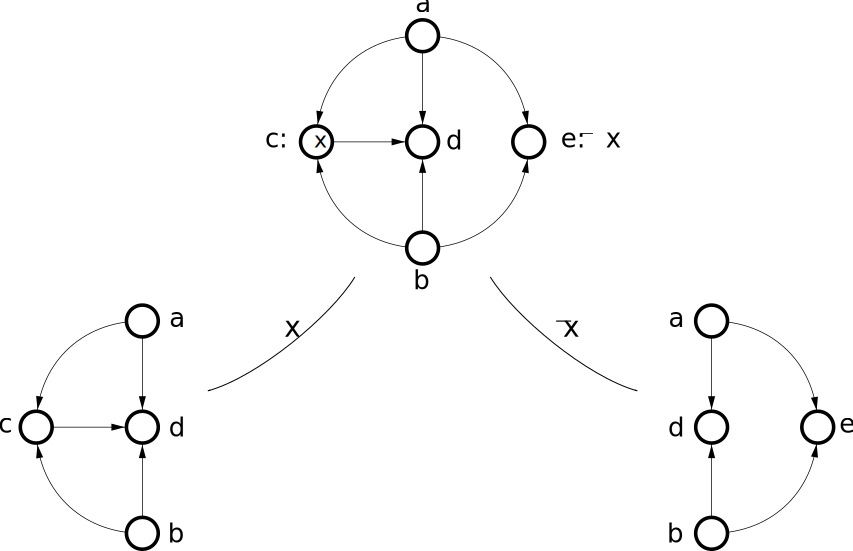
\includegraphics[width=1\columnwidth]{fig/cpog_projection_2_trans}
\par\end{centering}
\caption{The PG from Fig.~\ref{fig:Specialisations} simplified using the
Closure axiom, together with its specialisations\label{fig:The-simplified-CG-from}}
\end{figure}


By the same reasoning as in the previous section, we can conclude
that the following result holds.
\begin{thm}
[Soundness, Minimality and Completeness] The set of axioms of TPG-algebra
is sound, minimal and complete w.r.t. TPGs.
\end{thm}

\section{Case studies}

In this section we consider several practical case studies from hardware
synthesis. The advantage of (T)PG-algebra is that it allows for a
formal and compositional approach to system design. Moreover, using
the rules of (T)PG-algebra one can formally manipulate specifications,
in particular, algebraically simplify them.


\subsection{Phase encoders}

This section demonstrates the application of PG-algebra to designing
the \emph{multiple rail phase encoding} controllers\emph{~}\cite{2006_cdalessandro_async}.
They use several wires for communication, and data is encoded by the
order of occurrence of transitions in the communication lines. Fig.~\ref{fig:phase-encoding}(a)
shows an example of a data packet transmission over a 4-wire phase
encoding communication channel. The order of rising signals on wires
indicates that permutation $abdc$ is being transmitted. In total
it is possible to transmit any of the $n!$ different permutations
over an $n$-wire channel in one communication cycle. This makes the
multiple rail phase encoding protocol very attractive for its information
efficiency~\cite{2010_mokhov_ieee}. 

\begin{figure}
\begin{centering}
\hfill{}\subfloat[Phase encoded data]{\begin{centering}
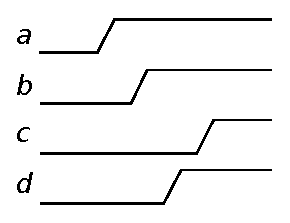
\includegraphics[scale=0.63]{fig/packet}
\par\end{centering}

}\hfill{}\subfloat[Matrix phase encoder]{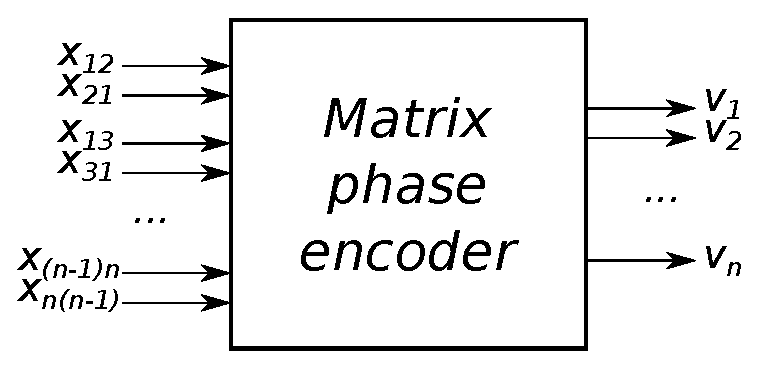
\includegraphics[scale=0.41]{fig/matrix_phase_encoder}



}\hfill{}
\par\end{centering}

\caption{Multiple rail phase encoding\label{fig:phase-encoding}}
\vspace{-6mm}
\end{figure}


Phase encoding controllers contain an exponential number of behavioural
scenarios w.r.t. the number of wires, and are very difficult for specification
and synthesis using conventional approaches. In this section we apply
PG-algebra to specification of an $n$-wire \emph{matrix phase encoder}
-- a basic phase encoding controller that generates a permutation
of signal events given a matrix representing the order of the events
in the permutation.

Fig.~\ref{fig:phase-encoding}(b) shows the top-level view of the
controller's structure. Its inputs are ${n \choose 2}$ dual-rail
ports that specify the order of signals to be produced at the controller's
$n$ output wires. The inputs of the controller can be viewed as an
$n\times n$ Boolean matrix $(x_{ij})$ with diagonal elements being
0. The outputs of the controller will be modelled by $n$ actions
$v_{i}\in\mathcal{A}$. Whenever $x_{ij}=1$, event~$v_{i}$ must
happen before event~$v_{j}$. It is guaranteed that $x_{ij}$ and
$x_{ji}$ cannot be 1 at the same time, however, they can be simultaneously
0, meaning that the relative order of the events is not known yet
and the controller has to wait until $x_{ij}=1$ or $x_{ji}=1$ is
satisfied (other outputs for which the order is already known can
be generated meanwhile). 

The overall specification of the controller is obtained as the overlay
${\displaystyle \sum_{1\le i<j\le n}}H_{ij}$ of fixed-size expressions
$H_{ij}$, modelling the behaviour of each pair of outputs. In turn,
each $H_{ij}$ is an overlay of three possible scenarios:
\begin{enumerate}
\item If $x_{ij}=1$ (and so $x_{ji}=0$) then there is a causal dependency
between $v_{i}$ and $v_{j}$, described using the PG-algebra sequence
operator: $v_{i}\rightarrow v_{j}$. 
\item If $x_{ji}=1$ (and so $x_{ij}=0$) then there is a causal dependency
between $v_{j}$ and $v_{i}$: $v_{j}\rightarrow v_{i}$. 
\item If $x_{ij}=x_{ji}=0$ then neither $v_{i}$ nor $v_{j}$ can be produced
yet; this is expressed by a circular wait condition between $v_{i}$
and $v_{j}$: $v_{i}\rightarrow v_{j}+v_{j}\rightarrow v_{i}$.%
\footnote{There are other ways to describe this scenario, e.g. by creating self-loops
$v_{i}\rightarrow v_{i}+v_{j}\rightarrow v_{j}$.%
} 
\end{enumerate}
We prefix each of the scenarios with its precondition and overlay
the results:
\[
\begin{array}{c}
H_{ij}=[x_{ij}\wedge\overline{x_{ji}}](v_{i}\rightarrow v_{j})+[x_{ji}\wedge\overline{x_{ij}}](v_{j}\rightarrow v_{i})+\\
+[\overline{x_{ij}}\wedge\overline{x_{ji}}](v_{i}\rightarrow v_{j}+v_{j}\rightarrow v_{i}).
\end{array}
\]
Using the rules of PG-algebra, we can simplify this expression to
\[
[\overline{x_{ji}}](v_{i}\rightarrow v_{j})+[\overline{x_{ij}}](v_{j}\rightarrow v_{i}),
\]
or, using the conditional sequence operator, to
\[
[\overline{x_{ij}}\vee\overline{x_{ji}}](v_{i}\overset{\overline{x_{ji}}}{\longrightarrow}v_{j}+v_{j}\overset{\overline{x_{ij}}}{\longrightarrow}v_{i}).
\]


Now, bearing in mind that condition $[\overline{x_{ij}}\vee\overline{x_{ji}}]$
is assumed to hold in the proper controller environment ($x_{ij}$
and $x_{ji}$ cannot be 1 simultaneously), we can replace it with
$[1]$ and drop it. The resulting expression can be graphically represented
as shown in Fig.~\ref{fig:CGs-related-to}(a). An example of an overall
controller specification ${\displaystyle \sum_{1\le i<j\le n}}H_{ij}$
for the case when $n=3$ is shown in Fig.~\ref{fig:CGs-related-to}(b).
The synthesis of this specification to a digital circuit can be performed
in a way similar to~\cite{2010_mokhov_ieee}.

\begin{figure}
\hfill{}\subfloat[$H_{ij}$]{

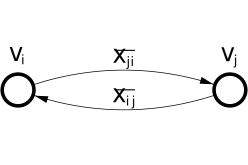
\includegraphics[scale=0.5]{fig/cpog_matrix_sender_ij}}\hfill{}\subfloat[$H_{12}+H_{13}+H_{23}$]{

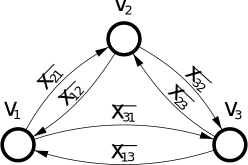
\includegraphics[scale=0.5]{fig/cpog_matrix_sender}}\hfill{}

\caption{PGs related to matrix phase encoder specification\label{fig:CGs-related-to}}
\vspace{-6mm}
\end{figure}



\subsection{Processor microcontroller and instruction set design}

This section demonstrates application of TPG-algebra to designing
processor microcontrollers. Specification of such a complex system
as a processor has to start at the architectural level, which helps
to manage the system complexity by structural abstraction~\cite{1994_de_micheli_book}.

Fig.~\ref{app-fig-Architecture-of-example} shows the architecture
of an example processor. Separate \emph{Program memory} and \emph{Data
memory} blocks are accessed via the \emph{Instruction fetch} (IFU)
and \emph{Memory access} (MAU) units, respectively. The other two
operational units are: \emph{Arithmetic logic unit} (ALU) and \emph{Program
counter increment unit} (PCIU). The units are controlled using request-acknowledgement
interfaces (depicted as bidirectional arrows) by the\textbf{\emph{
}}\emph{Central microcontroller}, which is our primary design objective. 

The processor has four registers: two general purpose registers $A$
and $B$, \emph{Program counter} (PC) storing the address of the current
instruction in the program memory, and the \emph{Instruction register}
(IR) storing the \emph{opcode} (operation code) of the current instruction.
For the purpose of this paper, the actual width of the registers (the
number of bits they can store) is not important. ALU has access to
all the registers via the register bus; MAU has access to general
purpose registers only; IFU, given the address of the next instruction
in PC, reads its opcode into IR; and PCIU is responsible for incrementing
PC (moving to the next instruction). The microcontroller has access
to the IR and ALU \emph{flags} (information about the current state
of ALU which is used in branching instructions).

Now we define the set of instructions of the processor. Rather than
listing all the instructions, we describe classes of instructions
with the same \emph{addressing mode}~\cite{mspmanual} and the same
execution scenario. As the scenarios here are partial orders of actions,
we use TPG-algebra, and the corresponding TPGs are shown in Fig.~\ref{app-fig-Scenarios-of-8}.

\textbf{ALU operation Rn to Rn}\quad{}An instruction from this class
takes two operands stored in the general purpose registers ($A$ and
$B$), performs an operation, and writes the result back into one
of the registers (so called \emph{register direct addressing mode}).
Examples: $\mathit{ADD\ A,\ B}$ -- addition $A:=A+B$; $\mathit{MOV\ B,\ A}$
-- assignment $B:=A$. ALU works concurrently with PCIU and IFU, which
is captured by the expression $\mathit{ALU}+\mathit{PCIU\rightarrow\mathit{IFU}}$;
the corresponding PG is shown in Fig.~\ref{app-fig-Scenarios-of-8}(a).
As soon as both concurrent branches are completed, the processor is
ready to execute the next instruction. Note that it is not important
for the microcontroller which particular ALU operation is being executed
($\mathit{ADD}$, $\mathit{MOV}$, or any other instruction from this
class) because the scenario is the same from its point of view (it
is the responsibility of ALU to detect which operation it has to perform
according to the current opcode). 

\begin{figure}
\begin{centering}
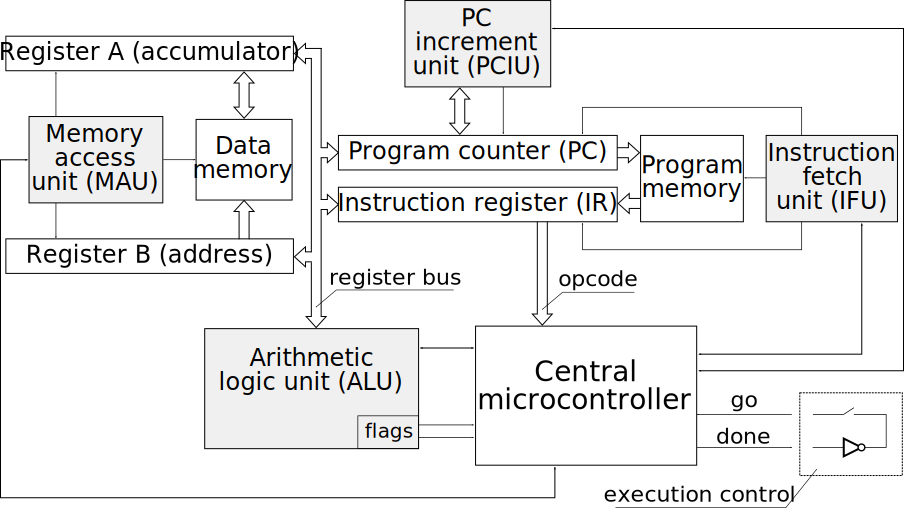
\includegraphics[width=1.04\columnwidth]{fig/processor_architecture}
\par\end{centering}

\caption{Architecture of an example processor\label{app-fig-Architecture-of-example}}
\vspace{-6mm}
\end{figure}


\begin{figure*}
\begin{centering}
\subfloat[ALU op. Rn to Rn]{

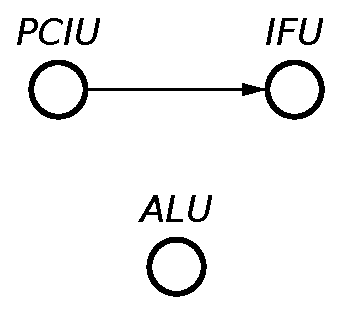
\includegraphics[scale=0.36]{fig/po_ALU_Rn_Rn}}\hfill{}\subfloat[ALU op. \#123 to Rn]{

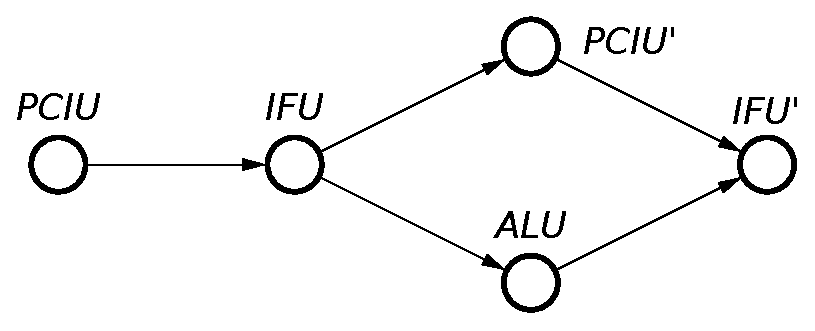
\includegraphics[scale=0.36]{fig/po_ALU_123_Rn}}\hfill{}\subfloat[ALU op. Rn to PC]{

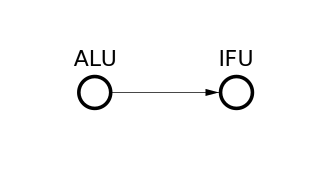
\includegraphics[scale=0.36]{fig/po_ALU_Rn_PC}}\hfill{}\subfloat[ALU op. \#123 to PC]{

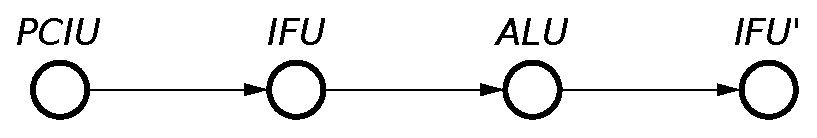
\includegraphics[scale=0.36]{fig/po_ALU_123_PC}}
\par\end{centering}

\begin{centering}
\subfloat[Memory access]{

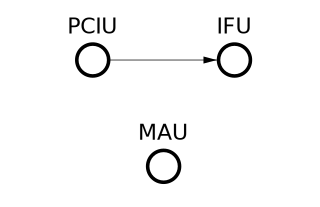
\includegraphics[scale=0.36]{fig/po_MAU}}\hfill{}\subfloat[Cond. ALU op. Rn to Rn]{

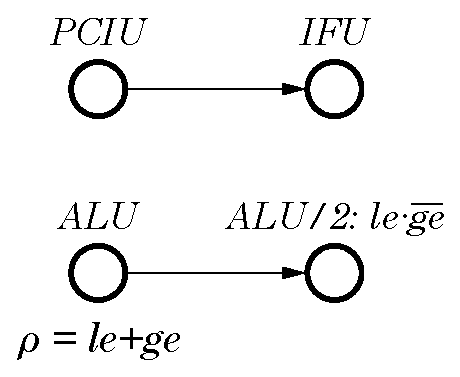
\includegraphics[scale=0.36]{fig/po_CALU_Rn_Rn}}\hfill{}\subfloat[Cond. ALU op. \#123 to Rn]{

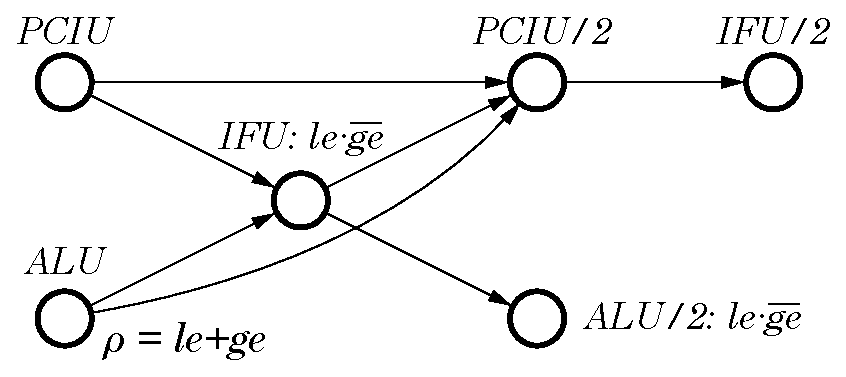
\includegraphics[scale=0.36]{fig/po_CALU_123_Rn}}\hfill{}\subfloat[Cond. ALU op. \#123 to PC]{

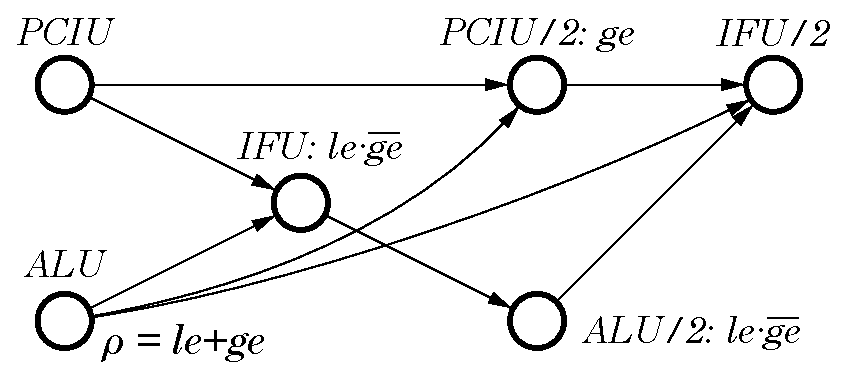
\includegraphics[scale=0.36]{fig/po_CALU_123_PC}}
\par\end{centering}

\caption{TPG specifications of instruction classes\label{app-fig-Scenarios-of-8}}
\vspace{-6mm}
\end{figure*}


\textbf{ALU operation \#123 to Rn}\quad{}In this class of instructions
one of the operands is a register and the other is a constant which
is given immediately after the instruction opcode (e.g. $\mathit{SUB\ A,\ \#5}$
-- subtraction $A:=A-5$), so called \emph{immediate addressing mode}.
At first, the constant has to be fetched into IR, modelled as $\mathit{PCIU}\rightarrow\mathit{IFU}$.
Then ALU is executed concurrently with another increment of PC: $\mathit{ALU}+\mathit{PCIU'}$
(we use $'$ to distinguish the different occurrences of actions of
the same unit). Finally, it is possible to fetch the next instruction
into IR: $\mathit{IFU'}$. The overall scenario is then $\mathit{PCIU}\rightarrow\mathit{IFU}\rightarrow(\mathit{ALU}+\mathit{PCIU'})\rightarrow\mathit{IFU'}$.

\textbf{ALU operation Rn to PC}\quad{}This class contains operations
for unconditional branching, in which PC register is modified. Branching
can be absolute or relative: $\mathit{MOV\ PC,\ A}$ -- absolute branch
to address stored in register $A$, $PC:=A$; $\mathit{ADD\ PC,\ B}$
-- relative branch to the address $B$ instructions ahead of the current
address, $PC:=PC+B$. The scenario is very simple in this case: $\mathit{ALU}\rightarrow\mathit{IFU}$.

\textbf{ALU operation \#123 to PC}\quad{}Instructions in this class
are similar to those above, with the exception that the branch address
or offset is specified explicitly as a constant. The execution scenario
is composed of : $\mathit{PCIU}\rightarrow\mathit{IFU}$ (to fetch
the constant), followed by an ALU operation, and finally by another
IFU operation, $\mathit{IFU'}$. Hence, the overall scenario is $\mathit{PCIU}\rightarrow\mathit{IFU}\rightarrow\mathit{ALU}\rightarrow\mathit{IFU'}$.

\textbf{Memory access}\quad{}There are two instructions in this class:
$\mathit{MOV\ A,\ [B]}$ and $\mathit{MOV\ [B],\ A}$. They load/save
register $A$ from/to memory location with address stored in register
$B$. Due to the presence of separate program and data memory access
blocks, this memory access can be performed concurrently with the
next instruction fetch: $\mathit{PCIU}\rightarrow\mathit{IFU}+\mathit{MAU}$.

\textbf{Conditional instructions}\quad{}These three classes of instructions
are similar to their unconditional versions above with the difference
that they are performed only if the condition $A<B$ holds. The first
ALU action compares registers $A$ and $B$, setting the ALU flag
$lt$ (less than) according to the result of the comparison. This
flag is then checked by the microcontroller in order to decide on
the further scheduling of actions. 

\textbf{Rn~to~Rn}\quad{}This instruction conditionally performs
an ALU operation with the registers (if the condition does not hold,
the instruction has no effect, except changing the ALU flags). The
operation starts with an ALU operation comparing $A$ with $B$; depending
on the result of this comparison, i.e. the status of the flag $lt$,
the second ALU operation may be performed. This is captured by the
expression $\mathit{ALU}\rightarrow[lt]\mathit{ALU'}$. Concurrently
with this, the next instruction is fetched: $\mathit{PCIU}\rightarrow\mathit{IFU}$.
Hence, the overall scenario is $\mathit{PCIU}\rightarrow\mathit{IFU}+\mathit{ALU}\rightarrow[lt]\mathit{ALU'}$.

\textbf{\#123~to~Rn}\quad{}This instruction conditionally performs
an ALU operation with a register and a constant which is given immediately
after the instruction opcode (if the condition does not hold, the
instruction has no effect, except changing the ALU flags). We consider
the two possible scenarios:
\begin{itemize}
\item $A<B$ holds: First, ALU compares $A$ and $B$ concurrently with
a PC increment; since $A<B$ holds, the ALU sets flag $lt$ and the
constant is fetched to the instruction register: $(\mathit{ALU}+\mathit{PCIU})\rightarrow\mathit{IFU}$.
After that PC has to be incremented again, $\mathit{PCIU'}$, and
ALU performs the operation, $\mathit{ALU'}$. Finally, the next instruction
is fetched (it cannot be fetched concurrently with $\mathit{ALU'}$
as ALU is using the constant in IR): $(\mathit{ALU'}+\mathit{PCIU'})\rightarrow\mathit{IFU'}$.
\item $A<B$ does not hold: First, ALU compares $A$ and $B$ concurrently
with a PC increment; since $A<B$ does not hold, the ALU resets flag
$lt$ and the constant that follows the instruction opcode is skipped
by incrementing the PC: $(\mathit{ALU}+\mathit{PCIU})\rightarrow\mathit{PCIU'}$.
Finally, the next instruction is fetched: $\mathit{IFU'}$.
\end{itemize}
\begin{figure*}
\centering{}\hspace*{\fill}%
\begin{tabular}{||c||||c||}
\hline 
{\small Instructions class} & {\small Opcode: $xyz$}\tabularnewline
\hline 
\hline 
{\small ALU Rn to Rn} & {\small 000}\tabularnewline
\hline 
{\small ALU \#123 to Rn} & {\small 110}\tabularnewline
\hline 
{\small ALU Rn to PC} & {\small 101}\tabularnewline
\hline 
{\small ALU \#123 to PC} & {\small 010}\tabularnewline
\hline 
{\small Memory access} & {\small 100}\tabularnewline
\hline 
{\small C/ALU Rn to Rn} & {\small 001}\tabularnewline
\hline 
{\small C/ALU \#123 to Rn} & {\small 111}\tabularnewline
\hline 
{\small C/ALU \#123 to PC} & {\small 011}\tabularnewline
\hline 
\end{tabular}\hspace*{\fill}\raisebox{-5em}[0em]{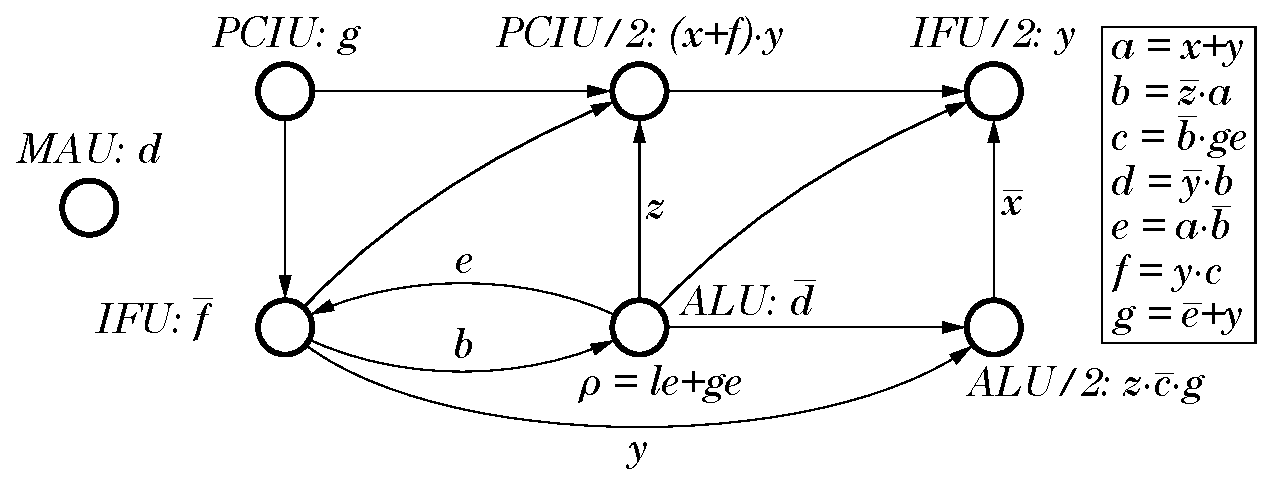
\includegraphics[scale=0.5]{fig/CPOG_L_3}}\hspace*{\fill}\caption{Optimal 3-bit instruction opcodes and the corresponding TPG specification
of the microcontroller\label{fig:opcodes-and-CG}}
\vspace{-6mm}
\end{figure*}


Hence, the overall scenario is the overlay of the two subscenarios
above prefixed with appropriate conditions (here we denote the predicate
$A<B$ by $lt$): 
\[
\begin{array}{c}
[lt]((\mathit{ALU}+\mathit{PCIU})\!\rightarrow\!\mathit{IFU}\!\rightarrow\!(\mathit{ALU'}+\mathit{PCIU'})\!\rightarrow\!\mathit{IFU'})+\\
+[\overline{lt}]((\mathit{ALU}+\mathit{PCIU})\!\rightarrow\!\mathit{PCIU'}\!\rightarrow\!\mathit{IFU'}).
\end{array}
\]
This expression can be simplified using the rules of TPG-algebra:%
\footnote{This case illustrates the advantage of using the new hierarchical
approach that allows to specify the system as a composition of scenarios
and formally manipulate them in an algebraic fashion. In the previous
paper~\cite{2011_mokhov_iet} the CPOG for this class of instruction
was designed monolithically, and because of this the arc between $\mathit{ALU'}$
and $\mathit{IFU'}$ was missed. Adding this arc not only fixes the
dangerous race between these two blocks, but also leads to a smaller
microcontroller due to the additional similarity between TPGs for
this class of instructions and for the one described below.%
}
\[
(\mathit{ALU}+\mathit{PCIU})\!\rightarrow\![lt]\mathit{IFU}\!\rightarrow\!(\mathit{PCIU'}+[lt]\mathit{ALU'})\!\rightarrow\!\mathit{IFU'}.
\]


\textbf{\#123~to~PC}\quad{}This instruction performs a conditional
branching in which the branch address or offset is specified explicitly
as a constant. We consider the two possible scenarios:
\begin{itemize}
\item $A<B$ holds: First, ALU compares $A$ and $B$ concurrently with
a PC increment; since $A<B$ holds, the ALU sets flag $lt$ and the
constant is fetched to the instruction register: $(\mathit{ALU}+\mathit{PCIU})\rightarrow\mathit{IFU}$.
After that ALU performs the branching operation by modifying PC, $\mathit{ALU'}$.
After PC is changed, the next instruction is fetched, $\mathit{IFU'}$.
\item $A<B$ does not hold: the scenario is exactly the same as in the \textbf{\#123~to~Rn
}case when $A<B$ does not hold.
\end{itemize}
Hence, the overall scenario is the overlay of the two subscenarios
above prefixed with appropriate conditions (here we denote the predicate
$A<B$ by $lt$): 
\[
\begin{array}{c}
[lt]((\mathit{ALU}+\mathit{PCIU})\!\rightarrow\!\mathit{IFU}\!\rightarrow\!\mathit{ALU'}\!\rightarrow\!\mathit{IFU'})+\\
+[\overline{lt}]((\mathit{ALU}+\mathit{PCIU})\!\rightarrow\!\mathit{PCIU'}\!\rightarrow\!\mathit{IFU'}).
\end{array}
\]
This expression can be simplified using the rules of TPG-algebra:
\[
(\mathit{ALU}+\mathit{PCIU})\!\rightarrow\!([\overline{lt}]\mathit{PCIU'}+[lt](\mathit{IFU}\!\rightarrow\!\mathit{ALU'}))\!\rightarrow\!\mathit{IFU'}.
\]


The overall specification of the microcontroller can now be obtained
by prefixing the scenarios with appropriate conditions and overlaying
them. These conditions can be naturally derived from the instruction
opcodes. The opcodes can be either imposed externally or chosen with
the view to optimise the microcontroller. In the latter case, TPG-algebra
and TPGs allow for a formal statement of this optimisation problem
and aid in its solving; in particular, the sizes of the TPG-algebra
expression or TPG are useful measures of microcontroller complexity
(there is a compositional translation from a TPG-algebra expression
into a linear-size circuit). In this paper we do not go into details
how to select the optimal encoding, but see~\cite{2011_mokhov_iet}.
We just note that it is natural to use three bits for opcodes as there
are eight classes of instructions, and give an example of optimal
3-bit encoding in the table in Fig.~\ref{fig:opcodes-and-CG}; the
TPG specification of the corresponding microcontroller is shown in
the right part of this figure (the TPG-algebra expression is not shown
because of its size).

\section{Machine-assisted Formalisation of Parametrised Graph Algebra}

While developing mathematical theories and proofs it is important to maintain logical soundness.
Even if the proof correctness may be obvious to its author, the peer researchers are often unable (because the proof is not detailed enough) or not willing (because the proof is too involved) to verify it rigorously.
To avoid such problems we have decided to encode the theory in a formal system so that only definitions would require careful inspection, with proofs being checked automatically.

This section uses Agda ~\cite{norell:thesis} -- a programming language and proof assistant based on the Martin-Löf type theory -- for formalization of
Parametrised Graphs theory. The section additionally describes the algorithm 
for conversion of PG formulae to normal form and shows that the correctness of the algorithm has been verified.

The section extensively uses the syntax of Agda and references several definitions from the Agda standard library ~\cite{agdalib}.


\DeclareUnicodeCharacter{949}{\varepsilon} % ε
\DeclareUnicodeCharacter{8702}{QQQQQQQQQQQQQQQQQQ} % QQQ
\DeclareUnicodeCharacter{737}{^{l}} % ˡ
\DeclareUnicodeCharacter{8759}{\colon\colon} % ∷

\newcommand{\seq}{\gg}
\newcommand{\hyp}{\text{-}}

%format Set = "\Q{Set}"
%format List = "\Q{List}"
%format × = "\Q{×}"
%format ⊎ = "\Q{⊎}"
%format ∘ = "\Q{∘}"
%format map = "\Q{map}"
%format flip = "\Q{flip}"
%format foldr = "\Q{foldr}"


%format + = "\D{+}"
%format _+_ = "\_" + "\_"
%format ⇾ = "\D{\seq}"
%format _⇾_ = "\_" ⇾ "\_"
%format ⇾-assoc ="\D{\seq{}assoc}"
%format +-assoc ="\D{+assoc}"
%format +-comm = "\D{+comm}"
%format ⇾-identityˡ = "\D{\seq{}identity^l}"
%format ⇾-identityʳ = "\D{\seq{}identity^r}"
%format distribʳ = "\D{distrib^r}"
%format distribˡ = "\D{distrib^l}"
%format decomposition = "\D{decomposition}"
%format ⇾ʳ = "\D{\seq{}_r}"
%format ⇾₁ = "\D{\seq{}_1}"
%format _⇾₁_ = "\_" ⇾₁ "\_"
%format _⇾ʳ_ = "\_" ⇾ʳ "\_"
%format ∷ = "\C{::}"
%format ε = "\D{\varepsilon}"
%format G = "\D{G}"
%format B = "\D{B}"
%format ≈ = "\D{≈}"
%format _≈_ = "\_" ≈ "\_"

\subsection{Graph Algebra}
We start with defining an algebra of non-parametrised graphs, to extend them with conditions later.

We define graph algebra as an algebraic structure over a set |G| with an equivalence relation |≈| supporting the following operations:
\begin{itemize}
\item{An empty graph, denoting no actions.
\begin{code}
ε : G
\end{code}}
\item{Graph overlay, denoting the parallel composition of actions from both graphs.
\begin{code}
_+_ : G → G → G
\end{code}}
\item{Graph sequencing, denoting the causal dependency between actions in the first graph and in the second graph.
\begin{code}
_⇾_ : G → G → G
\end{code}
}
\end{itemize}

Additionally, the operations must satisfy the following properties:

\begin{itemize}
\item{Overlay is commutative and associative.
\begin{code}
  +-assoc : ∀ p q r → (p + q) + r ≈ p + (q + r)
  +-comm : ∀ p q → p + q ≈ q + p
\end{code}}
\item{Sequencing is associative.
\begin{code}
  ⇾-assoc : ∀ p q r → 
    (p ⇾ q) ⇾ r ≈ p ⇾ (q ⇾ r)
\end{code}}
\item{Empty graph is a no-op in relation to sequencing.
\begin{code}
  ⇾-identityˡ : ∀ p → ε ⇾ p ≈ p
  ⇾-identityʳ : ∀ p → p ⇾ ε ≈ p
\end{code}}
\item{Sequencing distributes over overlay.
\begin{code}
  distribˡ : ∀ p q r → 
    p ⇾ (q + r) ≈ p ⇾ q + p ⇾ r
  distribʳ : ∀ p q r → 
    (p + q) ⇾ r ≈ p ⇾ r + q ⇾ r
\end{code}}
\item{Sequence of more than two actions may be decomposed into shorter sequences, 
forming the original sequence with overlay.
\begin{code}
  decomposition : ∀ p q r → 
                  p ⇾ q ⇾ r ≈ p ⇾ q + p ⇾ r + q ⇾ r
\end{code}}
\end{itemize}

\subsubsection{Derived theorems}

%format +-identity = "\D{+identity}"
%format +-idempotence = "\D{+idempotence}"
%format absorptionʳ = "\D{absorption^r}"
%format absorptionˡ = "\D{absorption^l}"

The following theorems has been derived from the axioms:

\begin{itemize}
\item{Empty graph is a no-op in relation to overlay.
\begin{code}
  +-identity : ∀ p → p + ε ≈ p
\end{code}}
\item{Overlay is idempotent.
\begin{code}
  +-idempotence : ∀ p → p + p ≈ p
\end{code}}
\item{Absorption.
\begin{code}
  absorptionˡ : ∀ p q → p ⇾ q + p ≈ p ⇾ q
  absorptionʳ : ∀ p q → p ⇾ q + q ≈ p ⇾ q
\end{code}}
\end{itemize}

\subsection{Parametrised Graphs}

%format ∧ = "\D{∧}"
%format _∧_ = "\_" ∧ "\_"
%format ∨ = "\D{∨}"
%format _∨_ = "\_" ∨ "\_"
%format ¬_ = ¬ "\_"
%format ¬ = "\D{¬}"
%format ⊤ = "\D{⊤}"
%format ⊥ = "\D{⊥}"

The graph algebra introduced in the previous subsection can only describe static event dependencies.
To describe complex dynamic systems one has to consider the conditional behaviour as well.
To do this, we have extended the graph algebra by annotating the graphs with conditions.
Given a set |G| of the parametrised graphs and a set |B| of all the possible boolean conditions, together with the following operations:

\begin{code}
  _∨_ : B → B → B
  _∧_ : B → B → B
  ¬ : B → B
  ⊤ : B
  ⊥ : B
\end{code}

we require a new operation called \emph{condition}:

%format cond0 = "\D{[}\_\D{]}\_"

\begin{code}
cond0 : B → G → G
\end{code}

The condition operation must have the following properties:

%format [ = "\D{[}"
%format ] = "\D{]}"
%format true-condition = "\D{true\hyp{}condition}"
%format false-condition = "\D{false\hyp{}condition}"
%format and-condition = "\D{and\hyp{}condition}"
%format or-condition = "\D{or\hyp{}condition}"
%format conditional-+ = "\D{conditional+}"
%format conditional-⇾ = "\D{conditional\!\seq}"

\begin{code}
  true-condition : ∀ x → [ ⊤ ] x ≈ x
  false-condition : ∀ x → [ ⊥ ] x ≈ ε
  and-condition : ∀ f g x → [ f ∧ g ] x ≈ [ f ] [ g ]  x
  or-condition : ∀ f g x → [ f ∨ g ] x ≈ [ f ] x + [ g ]  x
  conditional-+ : ∀ f x y → [ f ] (x + y) ≈ [ f ] x + [ f ] y
  conditional-⇾ : ∀ f x y → [ f ] (x ⇾ y) ≈ [ f ] x ⇾ [ f ] y
\end{code}

We say that there is a \emph{parametrised graph algebra} on a set |G| with a condition set |B|
if there is a graph algebra on |G|, a boolean algebra on |B| and a condition operator satisfying the requirements above.

\subsubsection{Derived Theorems}

The following theorems has been derived for the Parameterised Graph algebra.

%format choice-propagation₁ = "\D{choice\hyp{}propagation_1}"
%format choice-propagation₂ = "\D{choice\hyp{}propagation_2}"
%format condition-regularisation = "\D{condition\hyp{}regularisation}"

Choice propagation. If we have a choice between similar subgraphs, we can factor out the similarity and propagate choice onto the differing parts.
\begin{code}
choice-propagation₁ : ∀ b p q r → 
    [ b ] (p ⇾ q) + [ ¬ b ] (p ⇾ r) ≈ p ⇾ ([ b ] q + [ ¬ b ] r) 
choice-propagation₂ : ∀ b p q r → 
    [ b ] (p ⇾ r) + [ ¬ b ] (q ⇾ r) ≈ ([ b ] p + [ ¬ b ] q) ⇾ r
\end{code}

%format condition-regularisation = "\D{condition\hyp{}regularisation}"
%format condition-regularisationˢ = "\D{condition\hyp{}regularisation_s}"

Condition regularisation. A sequence of conditional events can be rewritten as an overlay of simpler terms.
\begin{code}
  condition-regularisation : ∀ f g p q → 
    [ f ] p ⇾ [ g ] q ≈ [ f ] p + [ g ] q + [ f ∧ g ] (p ⇾ q)
\end{code}

Strengthened condition regularisation. This generalizes the regularisation theorem by allowing any |z| containing all the edges between |p| and |q| to be used instead of |p ⇾ q|.
\begin{code}
  condition-regularisationˢ : ∀ f g p q z
                              → p ⇾ q ≈ p + q + z
                              → [ f ] p ⇾ [ g ] q ≈ [ f ] p + [ g ] q + [ f ∧ g ] z
\end{code}

\subsection{Parametrised Graph Formulae}

To perform automated manipulations of PG algebra formulae, we describe the formulae as an algebraic data type in the following way.

%format A = "\D{A}"
%format PGFormula = "\D{PGFormula}"

%format + = "\C{+}"
%format _+_ = "\_" + "\_"
%format ⇾ = "\C{\seq}"
%format _⇾_ = "\_" ⇾ "\_"
%format ε = "\C{ε}"
%format var = "\C{var}"
%format cond0 = "\C{[}\_\C{]}\_"
%format [ = "\C{[}"
%format ] = "\C{]}"

\begin{code}
 data PGFormula : Set where
  _+_ : (x y : PGFormula) → PGFormula
  _⇾_ : (x y : PGFormula) → PGFormula
  ε : PGFormula
  var : (a : A) → PGFormula
  cond0 : (c : B) → PGFormula → PGFormula
\end{code}

%format _+-s_ = "\_\D{+_s}\_"
%format _⇾-s_ = "\_\D{\seq_s}\_"
%format ε-s = "\D{ε_s}"
%format cond-s = "\D{[}\_\D{]_s}\_"
%format var-s = "\D{var_s}"

Here |A| is a set of graph variables and |B| is a set of condition variables.
We also have a constructor of |PGFormula| corresponding to each of the algebra operations and an additional constructor to reference the free variables.
This way we can construct the formulae in a straightforward way: 

\begin{code}
var "x" + var "y" ⇾ var "z"
\end{code}

%format pg-eval = "\D{pg\hyp{}eval}"

Formula evaluation then is catamorphism of PGFormula, replacing constructor applications with the corresponding algebra operations and |var| constructors with the actual variable values.
\begin{code}
pg-eval : {A B G : Set} 
   → (_+-s_ _⇾-s_ : G → G → G) 
   → (ε-s : G) 
   → (cond-s : B → G → G) 
   → (var-s : A → G) 
   → PGFormula A B 
   → G
\end{code}

%format BoolFormula = "\D{BoolFormula}"

%format ∧ = "\C{∧}"
%format _∧_ = "\_" ∧ "\_"
%format ∨ = "\C{∨}"
%format _∨_ = "\_" ∨ "\_"
%format ¬_ = ¬ "\_"
%format ¬ = "\C{¬}"
%format ⊤ = "\C{⊤}"
%format ⊥ = "\C{⊥}"

We use the same technique to define the |BoolFormula| data structure, with constructors |_∧_|, |_∨_|, |¬_|, |⊤|, |⊥| and |var|.

\subsection{Formula equivalence}

Naturally, it is possible to write the same mathematical function in many structurally different, but logically equivalent ways.
Here we define a notion of PG formula equivalence. We say that two formula are equivalent iff they 
can be structurally transformed one into the other by the set of rules corresponding to the equality rules of PG algebra.
We express this with an indexed inductive data family by explicitly enumerating all the important constructors.

%format ⇾-assoc ="\C{\seq{}assoc}"
%format +-assoc ="\C{+assoc}"
%format +-comm = "\C{+comm}"
%format V = "\D{V}"

\begin{code}
 data _≈_ : PGFormula (BoolFormula B) V 
         → PGFormula (BoolFormula B) V → Set where
  +-assoc : ∀ p q r → (p + q) + r ≈ p + (q + r)
  +-comm : ∀ p q → p + q ≈ q + p
  ⇾-assoc : ∀ p q r → (p ⇾ q) ⇾ r ≈ p ⇾ (q ⇾ r)
  ...
\end{code}

This definition allows for convenient formula manipulation, without mentioning its semantics.
However, the meaning of this definition is dubious because it was constructed manually without any mention of PG Algebra.
To connect the formulae equivalence with an algebra object equivalence, we have defined the proper equivalence relation on formulae, 
in terms of their semantics. We say that equivalent formulae must give equivalent results for any algebra they are evaluated in.

%%format let = "\K{let}"
%%format in = "\K{in}"
%format ≈ˢ = "\D{≈^s}"
%format PGAlgebra = "\D{PGAlgebra}"
%format eval = "\D{eval}"

\begin{code}
f1 ≈ˢ f2 = 
   ∀ G → (algebra : PGAlgebra G) → (f : V → G) → 
   eval algebra f f1 ≈ eval algebra f f2 
\end{code}

Here we assume that |eval algebra| applies |pg-eval| to all of the |algebra| operations.
Now we can show that our easier to use equivalence relation is equivalent to the semantics-based definition:

%format ≈→≈ˢ = "\D{≈→≈^s}"
%format ≈ˢ→≈ = "\D{≈^s→≈}"

\begin{code}
≈→≈ˢ : ∀ f g → f ≈ g → f ≈ˢ g
≈ˢ→≈ : ∀ f g → f ≈ˢ g → f ≈ g
\end{code}

\subsection{Normal Form}

%format BF = "\D{BF}"
%format PG = "\D{PG}"
%format NF = "\D{NF}"
%format Lit = "\D{Lit}"
%format Node = "\D{Node}"

We say that a normal form (|NF|) of PG formula (|PG|) is an overlay of literals (|Lit|) where each literal is a |Node| annotated with a condition and each node is either a variable (|V|) or two variables connected with a sequence operator. We encode these definitions assuming boolean formulae (|BF|) as conditions.

\begin{code}
Node = V ⊎ V × V
Lit = Node × BF
NF = List Lit
\end{code}

So far we have defined the structure of those types without formally saying anything about their semantics. We define the semantics for them by providing a corresponding Parametrised Graph Formulae (|PG|).

%format inj₁ = "\C{inj_1}"
%format inj₂ = "\C{inj_2}"
%format fromNode = "\D{fromNode}"
%format , = "\C{,}"
%format mkt = "\_\C{,}\_"

A |Node|, depending on its constructor, corresponds to either a single variable or two variables connected via the sequence operator.
\begin{code}
   fromNode : Node → PG
   fromNode (inj₁ x) = var x
   fromNode (inj₂ (x , y)) = var x ⇾ var y
\end{code}

A |Lit| of the form |(node , condition)| corresponds to the formula |[ condition ] node|.

%format fromLit = "\D{fromLit}"

\begin{code}
   fromLit : Lit → PG
   fromLit (node , cond) = [ cond ] fromNode node
\end{code}

|NF| corresponds to the overlay of all of its literals.

%format fromNF = "\D{fromNF}"

\begin{code}
   fromNF : NF → PG
   fromNF = foldr _+_ ε ∘ map fromLit
\end{code}


\subsection{Normalisation algorithm}

To automate the translation of formulae to normal form we have developed the algorithm presented in this subsection.

%format +-nf = "\D{+_{NF}}"
%format ⇾-nf = "\D{\seq_{NF}}"
%format _⇾-nf_ = "\_" ⇾-nf "\_"
%format _+-nf_ = "\_" +-nf "\_"
%format fromVar = "\D{fromVar}"
%format addCondition = "\D{addCondition}"
%format normalise = "\D{normalise}"

The top-level normalisation function traverses the PG formula recursively, normalising all of the subformulae and combining them with the appropriate functions (|_+-nf_| for |+|, |_⇾-nf_| for |⇾|, etc.).

\begin{code}
  normalise : PG → NF
  normalise = pg-eval
                _+-nf_
                _⇾-nf_
                []
                addCondition
                fromVar
\end{code}

The individual functions manipulating normal forms are implemented in the following way.

\begin{itemize}

\item{The normal form of |ε| is empty list.}
\item{The normal form of a variable literal |x| is a singleton list containing |[ ⊤ ] x|.
\begin{code}
  fromVar : V → NF
  fromVar x = (inj₁ x , ⊤) ∷ []
\end{code}}
\item{Overlay of two normal forms is concatenation of their literals.
\begin{code}
  _+-nf_ : NF → NF → NF
  a +-nf b = a ++ b
\end{code}}
\item{Sequence of two normal forms can be defined by applying the distributivity rules as a sum of pairwise sequencing of their literals.
\begin{code}
  _⇾ʳ_ : Lit → NF → NF
  lit ⇾ʳ [] = lit ∷ []
  lit ⇾ʳ (x ∷ xs) = (lit ⇾₁ x) + (lit ⇾ʳ xs)

  _⇾-nf_ : NF → NF → NF
  [] ⇾-nf b = b
  (h ∷ t) ⇾-nf b = (h ⇾ʳ b) + (t ⇾-nf b)
\end{code}}
%format newArrows = "\D{newArrows}"
%format vertices = "\D{vertices}"
%format ⊗ = "\Q{⊗}"
\item{Sequence of two literals |[ f ] p ⇾ [ g ] q| then can be defined as |[ f ] p + [ g ] q + [ f ∧ g ] r| where |r = newArrows p q| is the set of new arc nodes formed by sequencing the nodes |p| and |q|.
\begin{code}
  vertices : Node → List V
  vertices (inj₁ x) = x ∷ []
  vertices (inj₂ (x , y)) = x ∷ y ∷ []
  
  newArrows : Node → Node → List Node
  newArrows p q = 
    map inj₂ (vertices p ⊗ vertices q)
  
  _⇾₁_ : Lit → Lit → List Lit
  (p , f) ⇾₁ (q , g) = (p , f) ∷ (q , g) 
      ∷ (map (flip mkt (f ∧ g)) (newArrows p q))
\end{code}
Here |vertices n| is the list of graph vertices contained in node |n| -- one vertex when |n| is a vertex node and two vertices when |n| is an arc node.

|newArrows a b| then is a set of arc nodes connecting each of the vertices in |a| to each of the vertices in |b|.
}
\end{itemize}

%format +-correct = "\D{+correct}"
%format ⇾-correct = "\D{\seq{}correct}"
%format ⇾ʳ-correct = "\D{\seq_rcorrect}"
%format ⇾₁-correct = "\D{\seq_1correct}"
%format normalise-correct = "\D{normalise\hyp{}correct}"
%format newArrows-correct = "\D{newArrows\hyp{}correct}"

\subsubsection{Algorithm Correctness}
We define the correctness of normalisation by saying that the semantics of the resulting normal form must be equivalent to the original formula.
\begin{code}
  normalise-correct : ∀ f → f ≈ fromNF (normalise f)
\end{code}

To prove this theorem we had to prove several simpler statements.

Normal form overlay is correct.
That is, the semantics of concatenated normal forms is the overlay of their individual semantics.
\begin{code}
 +-correct : ∀ x y → 
   fromNF x + fromNF y ≈ fromNF (x +-nf y)
\end{code}
This follows from the monoid structure of overlay.

The normal form sequencing functions are correct.
\begin{code}
 ⇾-correct : ∀ x y → 
   fromNF x ⇾ fromNF y ≈ fromNF (x ⇾-nf y)
\end{code}
This relies on the right distributivity and the correctness of |⇾ʳ|.
\begin{code}
 ⇾ʳ-correct : ∀ x y → 
   fromLit x ⇾ fromNF y ≈ fromNF (x ⇾ʳ y)
\end{code}
This relies on the left distributivity and the correctness of |⇾₁|.
\begin{code}
 ⇾₁-correct : ∀ x y → 
   fromLit x ⇾ fromLit y ≈ fromNF (x ⇾₁ y)
\end{code}
The correctness of |⇾₁| is proven by the following chain of reasoning.
%format sumNodes = "\D{sumNodes}"
\begin{code}
    fromLit (x , f) ⇾ fromLit (y , g)
     ≈⟨ condition-regularisationˢ; newArrows-correct ⟩
    fromLit (x , f) + fromLit (y , g) 
        + [ f ∧ g ] sumNodes (newArrows x y)
     ≈⟨ propagating the condition to the literals ⟩
    fromLit (x , f) + fromLit (y , g) 
       + fromNF (map (flip mkt (f ∧ g)) (newArrows x y))
     ≈⟨ by +-assoc and definitions ⟩
    fromNF ((x , f) ⇾₁ (y , g))
\end{code}
The desired properties of the |newArrows| function are not as obvious as the properties of the other functions. We have formulated them as follows.
% \newpage
\begin{code}
  newArrows-correct : ∀ x y → 
     fromNode x ⇾ fromNode y ≈ 
     fromNode x + fromNode y 
                       + sumNodes (newArrows x y)
\end{code}

where |sumNodes = foldr _+_ ε ∘ map fromNode|. Our proof of this property is less than elegant. We manually enumerate all four cases (vertex and vertex, vertex and arc, arc and vertex, arc and arc) and prove four theorems individually, using the decomposition, commutativity and associativity axioms. It's likely possible to simplify the proof by treating the nodes as lists of sequenced vertices and prove by induction on those lists, instead of enumerating all the possible cases.



\section{Improved Parallel Composition}\label{sec_intro}



\subsection{Abstract}
Parallel composition of labelled Petri nets is a fundamental operation in modular design. It is often used to combine models of subsystems into a model of the whole system.
Unfortunately, the standard definition of parallel composition almost always yields a `messy' Petri net, with many implicit places, causing performance deterioration in tools that are based on structural methods. In this paper we propose an optimised algorithm for computing the parallel composition. It often produces nets with fewer implicit places, which are thus better suited for subsequent application of structural methods.

\subsection{Introduction}

Parallel composition (\aka synchronous product) of labelled
Petri nets is a fundamental operation in modular design. It is
often used to combine models of subsystems into a model of the
whole system. In particular, there is a nice correspondence
between parallel composition of Signal Transition Graphs
(STGs), a class of labelled Petri nets used for modelling
asynchronous circuits, and connecting circuits by wires. Hence
performing this operation efficiently is important in practice.

Unfortunately, the standard definition of parallel composition almost always yields a `messy' Petri net, with many implicit places (even if the component Petri nets did not have them). Some of these places are easy to remove (\eg duplicate places, which have the same pre- and postsets), but in general for removing others one needs full-blown model checking, which is infeasible if the resulting composition is large.
Although implicit places do not have noticeable effect on tools based on state space exploration, such as \petrify~\cite{ckkly97}, the performance of tools that are based on structural methods, such as \desij~\cite{Sch07}, often deteriorates.

Consider an example shown in Fig.~\ref{fi-motivating-example1},
which shows the STG specifications of two components (a,b) and
the specification of the environment (c). (The used short-hand
drawing notation for STGs is explained in
Sect.~\ref{sec_pn_basic}.) The model of the behaviour of the
entire system can be obtained by constructing the parallel
composition of these three STGs, which is shown in part (d) of
this figure. One can see that it contains a few implicit places
(which are not duplicate places); intuitively, they appear due
to repeated causality specifications for every signal: the one
coming from the component where this signal is an output, and
others --- from the components where it is an input. Removing
these places yields a much `cleaner' STG, coinciding with that
shown in Fig.~\ref{fi-motivating-example2}(d).

\begin{figure}[!tb]
    \centering
    \begin{minipage}[b]{0.4\columnwidth}
    \centering
        $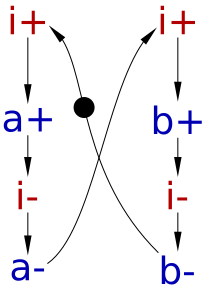
\includegraphics[scale=0.3]{EXPERIMENTS/stg/toggle}
        \atop
        \mbox{\rule[1.3em]{0em}{0em}(a) Toggle}$
        \\[0.5em]
        $\includegraphics[scale=0.3]{EXPERIMENTS/stg/mix}
        \atop
        \mbox{\rule[1.3em]{0em}{0em}(b) Call}$
        \\[0.5em]
        $\includegraphics[scale=0.3]{EXPERIMENTS/stg/env}
        \atop
        \mbox{\rule[1.3em]{0em}{0em}(c) Environment}$
    \end{minipage}
    $\includegraphics[scale=0.3]{EXPERIMENTS/stg/simple_standard}
    \atop
    \mbox{\rule[1.3em]{0em}{0em}(d) Composition}$
    \caption{\label{fi-motivating-example1}
        Example of standard STG composition.
    }
\end{figure}

\begin{figure}[!tb]
    \centering
    \begin{minipage}[b]{0.4\columnwidth}
        \centering
        $\includegraphics[scale=0.3]{EXPERIMENTS/stg/toggle_opt}
        \atop
        \mbox{\rule[1.3em]{0em}{0em}(a) Toggle}$
        \\[0.5em]
        $\includegraphics[scale=0.3]{EXPERIMENTS/stg/mix_opt}
        \atop
        \mbox{\rule[1.3em]{0em}{0em}(b) Call}$
        \\[0.5em]
        $\includegraphics[scale=0.3]{EXPERIMENTS/stg/env_opt}
        \atop
        \mbox{\rule[1.3em]{0em}{0em}(c) Environment}$
    \end{minipage}
    $\includegraphics[scale=0.3]{EXPERIMENTS/stg/simple_improved}
    \atop
    \mbox{\rule[1.3em]{0em}{0em}(d) Composition}$
    \caption{\label{fi-motivating-example2}
        Example of improved STG composition: the components are obtained from the corresponding ones in Fig.~\ref{fi-motivating-example1} by removing some places, and then the standard parallel composition is applied to these modified components.
    }
\end{figure}


One operation where implicit places matter is \emph{transition contraction,}~\cite{vowo02lncs} which is a crucial part of the re-syn\-the\-sis approach~\cite{CN-02,KVL-96,PC-96}. The idea is to hide the internal communication between the components (by labelling the corresponding transitions as `dummy' --- they correspond to signals $a$ and $b$ in our example), contract as many of these dummy transitions as possible (whereby reducing the size of the STG), and re-synthesise the obtained STG as a circuit (which is often smaller than the original circuit due to removal of some signals). Transition contraction has to be performed on very large STGs (corresponding to the whole control path of the circuit), and so, for efficiency, it has to be a structural operation. Unfortunately, such structural contractions are not always possible (see Sect.~\ref{sec_pn_basic}), and implicit places in the preset and/or postset of a transition can prevent contracting it, even if a contraction is possible after removing these implicit places. In our example, \desij cannot contract any of the dummy transitions in the STG in Fig.~\ref{fi-motivating-example1}(d), even though it performs some structural tests for place redundancy; however, it is able to contract all the dummy transitions if the implicit places are removed, \ie when applied to the STG in Fig.~\ref{fi-motivating-example2}(d).

The main contribution of this paper is a new me\-thod for computing the parallel composition of labelled Petri nets, that generates fewer implicit places. It uses the \emph{freeness from computation interference (FCI)} assumption, stating that the situation when one component wants to produce an output, but is prevented from doing so by another component which is not ready to receive it, is impossible. Violation of FCI means that the behaviour of the composition does not correspond to that of the physical system. For example, an output of a circuit component cannot be physically disabled by another component that is not ready to receive this signal, and so producing this output will lead to malfunction; however, the composition will be oblivious to it, and behave as if such an output could not be produced.
Hence FCI is a basic correctness requirement --- if it is violated, there is no point in computing parallel composition, as its behaviour will not describe that of the physical system. In practice, FCI is often guaranteed by construction, \eg it is always guaranteed for the control path of a \balsa~\cite{EB-02} or \haste/\tangram~\cite{berkel91,haste-manual} specification of an asynchronous circuit. The idea of using the FCI condition is reminiscent of the method of input/output exposure in the synthesis by direct mapping described in~\cite{SBY-07}, and of the correct by construction composition of Petri nets for circuit components and the environment used in the \ditopn tool~\cite{JF-00}.

The main idea of the method we propose here is illustrated by the example in Fig.~\ref{fi-motivating-example2}. Before doing the parallel composition, one can remove some of the places in the components as shown in parts (a--c) of the figure and then compose the modified STGs. The precise conditions that allow to remove a particular place will be stated in Sect.~\ref{se-main}; at this point it is only important that they are structural and thus can be efficiently checked. This guarantees that the number of places in the resulting Petri net is smaller (as the number of places in the composition is the total number of places in all the components), and, under the FCI assumption, the resulting behaviour will be the same (in the sense of isomorphism of the reachability graphs). In particular, in our example, composing the modified components yields the STG in Fig.~\ref{fi-motivating-example2}(d), which in this case contains no implicit places. Observe that the modified components on their own can have rather bad behaviour and in particular can be non-implementable; however, it does not matter, as they are never used on their own, but only in composition with other components, and the resulting behaviour of the composition is guaranteed to correspond to that of the standard composition.

Re-synthesis of asynchronous circuits is the intended application of the proposed method. However, we envisage that it has a much wider applicability, as composition of labelled Petri nets is a fundamental operation, and the FCI assumption often holds in practice.


\input{agda-processed-body}

%% \section{Redundancy in the Petri Nets produced by composition}

%% \section{Eliminating redundancy}

%% \section{Experimental results}

%% \section{Conclusions}

%% \chapter{CPOG Encoding}

\chapter{Processor instruction set encoding}

Main contributions of this chapter are: firstly, it formulates several
instruction set encoding problems in terms of the TPG model; secondly,
it presents the SAT characterisation of the problems leading to their
efficient automated solution; thirdly, it demonstrates application
of the TPG methodology at different stages of a processor design
flow --- from architectural-level specification, design and behavioural
description of an instruction set to its encoding and synthesis of
the physical implementation of the microcontroller. The chapter is organised
as follows. Section~\ref{sec:pg-encoding-problem-statement} introduces
the TPG encoding problem, overviews the existing encoding techniques and gives
a brief introduction to the new technique of globally optimal encoding.
A method for automated translation of the problems into SAT instances
is explained in Section~\ref{sec:SAT-formulation}. It is followed
by a processor design and synthesis example in Section~\ref{sec-processor} and
conclusions.

\label{chap:PGEncoding}

The chapter is based on the results published in~\cite{cpog_encoding}. It shows how to represent processor instruction sets using TPG formalism and provides
a ground for a concise formulation of several encoding problems, which
are reducible to the well-known Boolean satisfiability (SAT) problem
and can be efficiently solved by modern SAT solvers. Application of
all the presented techniques is demonstrated on a processor design
example.

\section{Problem statement\label{sec:pg-encoding-problem-statement}}
In microcontroller design, the encoding of an instruction set is a common reoccuring problem. A form of encoding optimality is essential to achieve a more compact instruction decoder logic, while, at the same time, offering higher decoding performance. The first step is to represent each instruction microcode as a TPG \emph{scenario}. Such scenario is a program each instruction of each is a reference to a microcontroller unit. The directed graph semantics underlaying PGs expresses the casual dependendencies between events of unit firings; informally, this means that instruction execution steps may be ordered sequentially or concurrently.   


An encoding scheme must ensure that every scenario is adeqautely represented in the composed graph. This property, called the \emph{encoding correctness condition}, is formulated by the following statement

$$
S_i = G \mid_{X = \theta_i} 
$$

\noindent
here $X$ is the set of free variables of PG $G$ (Chapter~\ref{chap:PGAlgebra}), $S_i$ is a scenario from a scenario set $S$ and $X = \theta_i$ stands for $\bigwedge_{x \in X} \mathsf{x} = \theta_i(x)$. The condition states that a scenario is properly decoded by applying an opcode-defined graph specialisation $\theta$. Every encoding schema may be characterised by a specific choice of set $X$ and encoding function $\theta$. We refer to a tuple of $(X, \theta)$ as encoding of a scenario set $S$.


To uniquely determine, upto PG equivalence, and for encoding and scenario set a compositional graph $G$ one also needs to consider the \emph{property of composition minimality}: 

$$
G = \sum_{i < n} [X = \theta_i](G \mid_{X = \theta_i}) 
$$

\noindent
Informally, the condition states that $G$ does not contain anything in addition to the encoding of scenarios $S$.

To give an intuition behind encoding we shall consider a simple case of encoding for two scnearios $S_1, S_2$. This encoding is constructed by putting together, in a certain manner, graphs $S_1$ and $S_2$. More precisely, we overlay the graphs of $S_1$ and $S_2$ using the $+$ operator: 

$$
G \DEF [X = \theta_1]S_1 + [X = \theta_2]S_2
$$

\noindent
The overlaid graphs are conditioned by their opcodes. In the above, $\theta_1, \theta_2$ is a unique value of vector $X$ identifying a given scenario. 

In a general case, for $n$ scenarios, this statement takes the following form:

$$
G \DEF \sum_{i < n} [X = \theta_i]S_i 
$$

\noindent
Such encoding constructing preserves the property of composition mininimality provided the correctness property also holds. Let us now briefly consider one particilar encoding scheme - the \emph{one hot} encoding - to the composition of scenarios $S_1, S_2$: 

$$
G \DEF [\mathsf{x}_1 = 1 \wedge \mathsf{x}_2 = 0]S_1 + [\mathsf{x}_1 = 0 \wedge \mathsf{x}_2 = 1]S_2
$$

\noindent
It is easy to check that one hot encoding satisfies the correctness condition. For instance, for the case of scenario $S_1$, we can prove that the scenario can be obtained via graph $G$ specialisation as follows:


$$
S_1 = ([\mathsf{x}_1 = 1 \wedge \mathsf{x}_2 = 0]S_1 + [\mathsf{x}_1 = 0 \wedge \mathsf{x}_2 = 1]S_2) \mid_{\mathsf{x}_1 = 1 \wedge \mathsf{x}_2 = 0}
$$

\noindent
which is obviously correct by the definition of the specialisation operator $H|_p$.


A common measure of complexity of a Boolean formula $f$ is denoted
as $C(f)$ and is defined to be the total count of literals in it,
e.g. $C(x\cdot z+y\cdot\overline{z})=4$, $C(1)=0$, etc. 
This is the metric used in \cite{2009_mokhov_phd} to assess the produced encodings.
Indeed, when applied to a single formula this metric often works well:
the more literals the formula has, the larger the circuit to evaluate this formula.
However, when used to assess multiple similar formulae or a single formula with repeating sub-formulae,
this metric fails to account for the fact that the outputs of logic gates evaluating the subformulae
can be reused. To take advantage of this fact we use the new metric $G(C)$, showing the total number of
 gates in the circuit needed to compute all of the conditions found in $C$.
We use two versions of this metric, differing in type of gates allowed: one with AND/OR gates with 
all possible input and output inversions and another one with NAND-gates only.

\subsection{Overview}

In this section we briefly discuss the encoding approaches developed in \cite{2009_mokhov_phd}. We implement as SAT-based solution for the pre-existing techniques (weakly optimal encoding) and introduce a new, more powerful technique for identifying globally optimal solutions. 

\subsubsection{One hot}

The one hot encoding scheme associates a unique indicator variable (a hot wire) with each scenario. The set of free variables is exactly that of the scenarios being encoded:

$$
X = \mathbf{S}
$$

\noindent
where $\mathbf{S}$ is the scenario set. The encoding is very simple: one sets $i$-th bit to 1 to select an $i$-th scenario and the rest must be reset to zero:

$$\theta_i(s) = (S_i = s), \quad \text{where} ~ s, S_i \in \mathbf{S}$$


\subsubsection{Matrix encoding}

The matrix encoding allocates a unique variable for each edge and vertex of scenario graphs $S_i$. Hence, the set of free variables is given as

$$
X = \{0\}\times V \cup \{1\} \times  E
$$

\noindent
An encoding bit is set depending on whether a given edge or vertex are included in a given scenario $s$: 
 
$$
\begin{array}{l}
\theta_i(0, v) = C_i(v), \quad \text{where} ~ v \in V_i \\
\theta_i(1, e) = D_i(e), \quad \text{where} ~ e \in E_i  
\end{array}
$$

\noindent
where scenario $S_i$ is defined by a PG of the form $(V_i, E_i, C_i, D_i, X_i)$.

\subsubsection{Binary encoding}

Binary encoding associates a scenario index with the value of binary number coded by an instruction opcode. One specific form of $X$ can be given as    

$$
X = 1 .. \lceil \log | \mathbf{S} | \rceil
$$

\noindent
where $\mathbf{S}$ is the scenario set.


The encoding function computes the $k$-th bit of $i$-th scenario opcode as a binary encoding of a natural number representing the scenario index:
 
$$\theta_i(k) = \left \lfloor {i - 1 \over {2^{k-1}}} \right \rfloor ~\mathrm{mod}~2, \quad \text{where} ~ k ~ \text{is the bit position}$$

\subsubsection{Weakly optimal\label{sec:weakly-optimal-encoding}}

The optimal encoding with unconstrained code length, which we call weakly optimal encoding, tries to minimize the size of set $X$ within the universe of solutions with 1-restricted conditions. We say that a graph is 1-restricted if all the edge and vertex conditions contain at most one literal. It has been showin in \cite{2009_mokhov_phd} that the problem of computing a weakly optimal encoding is NP-complete thus barring any attempts at brute force solutions. It is challenging to give a compact characterisation of optimal encoding in the terms of free variable set $X$ and coding function $\theta$. In the continuation of the Chapter we shall give a SAT formulation of this encoding approach. 


\subsection{Globally optimal encoding\label{Sec:Generating-optimal-opcodes}}

The weakly optimal encoding method presented above generates the smallest
PG description of a set of partial orders but the number of used
variables cannot be controlled; in many practical cases it will use
more variables than is affordable under the design or technology constraints.
In this section we briefly describe a method for generating the smallest
PG given a limit on the number of variables, i.e. given the required
length of the instruction codes.

Let $L$ be the given limit on the number of variables. We generate all non-trivial
encoding constraints and try to satisfy them with opcode variables.
Only $L$ of them are free variables $X=\{x_{1},\ x_{2},\ ...,\ x_{L}\}$;
other variables $F=\{f_{1},\ f_{2},\ ...,\ f_{m}$\} are not free
--- they are expressed in terms of variables from $X\cup F$ using
Boolean binary functions, e.g. $f_{1}=x_{1}+\overline{x_{3}}$, $f_{2}=f_{1}\cdot x_{2}$,
etc. As $L$ is fixed all we have to do is to minimise the number
of non-free variables $m$. This minimisation problem requires exploration
of large search space; fortunately, it still belongs to the NP complexity
class and we can reduce it to the SAT problem: the solver has to `guess'
all the opcodes, formulae of variables in $F$, and allocation of
all variables $X\cup F$ to the non-trivial encoding constraints.


\section{SAT formulation\label{sec:SAT-formulation}}

This section presents SAT formulations of the optimal encoding problems
described in the previous section.

The Boolean satisfiability problem (SAT) is to decide whether a given
Boolean formula $F(x_{1},\ x_{2},\ \dots,\ x_{n})$ is satisfiable
or not, i.e. if it is possible to find an assignment of Boolean values
$(\alpha_{1},\ \alpha_{2},\ \dots,\ \alpha_{n})\in\{0,\ 1\}^{n}$
to the variables $(x_{1},\ x_{2},\ \dots,\ x_{n})$ which makes the
formula true: $F(\alpha_{1},\ \alpha_{2},\ \dots,\ \alpha_{n})=1$.
As SAT is a decision (not optimisation) problem, we define a cost
function and use a binary search to minimise its value by calling
the SAT solver with different cost constraints.

We have implemented all the techniques presented in this section in
an automated software tool which uses \noun{MiniSat}~\cite{2004_miniSAT_lncs} and \noun{clasp}~\cite{clasp}
as SAT solver engines. They operate on CNF (conjunctive
normal form) representations of Boolean formulae. Since our SAT-instances
are not necessarily given in CNF, we implemented their automated conversion
to CNF formulae. This conversion introduces intermediate variables
but the overall size of the obtained formula is linear with respect
to the size of the given SAT-instance.



\subsection{Weakly optimal encoding}

To solve the weakly optimal encoding problem described 
in Subsection~\ref{sec:pg-encoding-problem-statement}
we minimise the number of colours used for a conflict graph colouring.
Minimisation is performed by solving a series of instances of the
following decision problem.

Let $G=(V,\ E)$ be an extended conflict graph, where vertices $V$
correspond to encoding constraints and edges $E\subseteq V\times V$
to conflicts between them. $V$ contains both original $V_{o}=\{\mathbf{e}_{1},\ \mathbf{e}_{2},\ \dots,\ \mathbf{e}_{n}\}$
and inverted $V_{i}=\{\mathbf{\overline{\mathbf{e}}}_{1},\ \mathbf{\overline{\mathbf{e}}}_{2},\ \dots,\ \mathbf{\overline{\mathbf{e}}}_{n}\}$
constraints, such that $V=V_{o}\cup V_{i}$. The problem is to find
a colouring of $G$ which uses no more than $m$ colours.

For every pair of vertices $(\mathbf{e}_{k},\ \mathbf{\overline{\mathbf{e}}}_{k})$
we introduce a Boolean variable $p_{k}$ and an integer number $c_{k}$
whose values have to be found by the SAT solver: $p_{k}$ indicates
which of the two vertices is coloured -- if $p_{k}=1$ (resp. $p_{k}=0$)
then $\mathbf{e}_{k}$ (resp. $\overline{\mathbf{e}}_{k}$) is coloured,
while $c_{k}$ represents the colour of the chosen vertex. 

The SAT problem $\mathcal{ENCODE}$ consists of four constraints:
\[
\mathcal{ENCODE}=\mathcal{NUM}\cdot\mathcal{COL}_{oo}\cdot\mathcal{COL}_{oi}\cdot\mathcal{COL}_{ii}
\]
where $\mathcal{NUM}$ restricts colours such that $0\le c_{k}<m$.
Encoding of numbers $c_{k}$ in Boolean domain can be different, for
example, if we use binary encoding we need $\left\lceil \log_{2}m\right\rceil $
bits for each $c_{k}$. Implementation of $\mathcal{NUM}$ depends
on the chosen encoding; its general form is:
\[
\mathcal{NUM}=\prod_{1\le k\le n}(0\le c_{k})\cdot(c_{k}<m)
\]
Constraints $\mathcal{COL}$ check that adjacent vertices are assigned
different colours:
\[
\mathcal{COL}_{oo}=\prod_{(\mathbf{e}_{j},\ \mathbf{e}_{k})\in E\cap(V_{o}\times V_{o})}(p_{j}\cdot p_{k})\Rightarrow(c_{j}\neq c_{k})
\]
\[
\mathcal{COL}_{oi}=\prod_{(\mathbf{e}_{j},\ \overline{\mathbf{e}}_{k})\in E\cap(V_{o}\times V_{i})}(p_{j}\cdot\overline{p_{k}})\Rightarrow(c_{j}\neq c_{k})
\]
\[
\mathcal{COL}_{ii}=\prod_{(\overline{\mathbf{e}}_{j},\ \overline{\mathbf{e}}_{k})\in E\cap(V_{i}\times V_{i})}(\overline{p_{j}}\cdot\overline{p_{k}})\Rightarrow(c_{j}\neq c_{k})
\]
If we assume that complexity of comparison operations over numbers
$c_{k}$ is $C$, then the overall complexity of $\mathcal{ENCODE}$
is $\Theta((|V|+|E|)\cdot C)$. In particular, in case of binary encodings%
\footnote{Formula $(a<b)$ for binary numbers comparison is $(a<b)=\overline{a_{0}}\cdot b_{0}+(a_{0}=b_{0})\cdot(a'<b')$
where $a'$ and $b'$ are obtained from $a$ and $b$ by removal of
their most significant digits ($a_{0}$ and $b_{0}$); the formula
is linear with respect to the lengths of $a$ and $b$.%
} the complexity is $\Theta((|V|+|E|)\cdot\log m)$. Depending on the
chosen number encodings, there are from $\Theta(|V|\cdot\log m)$
to $\Theta(|V|\cdot m)$ free variables.

If $L$ is the minimum value of $m$ for which formula $\mathcal{ENCODE}$
is satisfiable then the optimal encoding uses $L$ variables $X=\{x_{1},\ x_{2},\ ...,\ x_{L}\}$.
Values $p_{k}$ and $c_{k}$ which satisfy the formula are used to
resolve encoding constraints $\mathbf{e}_{k}$ in the following way:
if $p_{k}=1$ then $\mathbf{e}_{k}$ is resolved by $x_{c_{k}}$,
otherwise it is resolved by $\overline{x_{c_{k}}}$.


\subsection{Globally optimal encoding}

The version of the optimal encoding problem with constrained code length
is significantly more complicated and computationally intensive. It
requires finding a set of Boolean functions of $L$ arguments (where
$L$ is the specified code length) and there are $2^{2^{L}}$ of them
-- it is impossible to explore search spaces of such magnitudes, e.g.
$2^{2^{8}}$ roughly equals to the number of atoms in the universe.
To cope with this, we reduce the search space to 2-argument Boolean
functions only. From the practical point of view this is justified
by the fact that most modern technology libraries contain only 2-
or 3-input logic gates anyway. Importantly, every complex function
can be represented as a composition of simpler ones, therefore our
approach can find any function, albeit at the cost of introducing
intermediate variables. This is similar to what actually happens during
technology mapping and logic decomposition of
functional components into hardware gates~\cite{2002_cortadella_book}\cite{1994_de_micheli_book}.

Formally, let $(\mathbf{e}_{1},\ \mathbf{e}_{2},\ \dots,\ \mathbf{e}_{n})$
be a set of encoding constraints defined in Subsection~\ref{sec:pg-encoding-problem-statement},
$S$ be the number of scenarios, and $L$ be the required code length.
We are looking for such a vector $(\psi_{1},\ \psi_{2},\ \dots,\ \psi_{S})$
of $L$-bit encodings and $n$ functions $F_{j},\ 1\le j\le n$ such
that $F_{j}(\psi_{k})=\mathbf{e}_{j}[k]$ for every scenario $1\le k\le S$
(unless $\mathbf{e}_{j}[k]$ is a don't care value).

We represent a set of functions $F$ as a combinational circuit consisting
of $G$ 2-input Boolean gates, where $G$ is the value to be minimised.
An output of the circuit can be taken directly from one of its inputs
or be produced by a gate. In addition, any output can be inverted:
\[
F_{j}(\psi)=\mathit{select}(Signals(\psi),\ \mathit{oSelector}_{j})\oplus\mathit{Inv}_{j}
\]


Here $Signals(\psi)$ is a function computing all circuit signals
including both circuit inputs (given by parameter $\psi$) and gate
outputs, $\mathit{oSelector}_{j}$ is the number indicating which
circuit signal is `connected' to the $j$-th circuit output, function
$\mathit{select(V,\ k)}$ selects $k$-th element from a given vector
$V$, and $Inv_{j}=1$ iff $j$-th circuit output is inverted. Implementation
of function $select(V,\ k)$ depends on the encoding of $k$ (we used
one-hot encoding in this case, which allows for simpler implementation).
Circuit signals are computed as follows:
\[
\begin{cases}
\mathit{Signals}(\psi) & =\mathit{Wires}_{G}(\psi)\\
\mathit{Wires}_{k}(\psi) & =\begin{cases}
\psi & \textrm{\,\,\ if}\, k=0\\
\mathit{Wires}_{k-1}(\psi)\circ\mathit{Gate}_{k}(\psi) & \textrm{\,\,\ if}\,0<k\le G
\end{cases}\\
\mathit{Gate}_{k}(\psi) & =\mathit{arg}_{1,k}(\psi)\cdot\mathit{arg}_{2,k}(\psi)\\
\mathit{arg}_{j,k}(\psi) & =select(\mathit{Wires}_{k-1}(\psi),\ \mathit{aSelector}_{j,k})\oplus\mathit{InvArg}_{j,k}
\end{cases}
\]
In other words, a set of wires is initially equal to the set of circuit
inputs $(\mathit{Wires}_{0}(\psi)=\psi)$ and then is iteratively
extended by appending $Gate_{k}$ to the previously computed set of
wires $Wires_{k-1}$. Eventually, after $G$ iterations we obtain
the set of all signals $\mathit{Signals}(\psi)=\mathit{Wires}_{G}(\psi)$.
Every $Gate_{k}$ corresponds to an AND gate with possible input inversions
(indicated by $\mathit{InvArg}_{0,k}$ and $\mathit{InvArg}_{1,k}$).
Its arguments are selected by $\mathit{aSelector}_{0,k}$ and $\mathit{aSelector}_{1,k}$
from the set of wires computed in the previous iteration. This guarantees
the absence of combinational loops.

As every signal in the circuit can be optionally inverted (by setting
$\mathit{Inv}_{j}=1$ or $\mathit{InvArg}_{j,k}=1$), the resultant
gate basis includes 8 logic gates: AND, OR, NAND, NOR, plus 4 other
gates, obtained from these by inversion of exactly one of their inputs
(they do not have commonly adopted names, apart, perhaps, from Boolean
implication $x\Rightarrow y$ which corresponds to OR($\overline{x}$,
$y$)). We have also investigated a simpler basis, consisting of only
NAND gates with no optional input inversions. The basis leads to smaller
search space and works faster, but, as expected, produces larger circuits
(see Figure~\ref{fig:Comparison-of-different} for a comparison of
two bases on a processor example). If the NAND basis is used then
free variables $\mathit{InvArg}_{j,k}$ can be dropped and the formulae
for $\mathit{Gate}_{k}(\psi)$ and $\mathit{arg}_{j,k}(\psi)$ should
be modified as follows: 
\[
\begin{cases}
\mathit{Gate}_{k}(\psi) & =\overline{\mathit{arg}_{1,k}(\psi)\cdot\mathit{arg}_{2,k}(\psi)}\\
\mathit{arg}_{j,k}(\psi) & =select(\mathit{Wires}_{k-1}(\psi),\ \mathit{aSelector}_{j,k})
\end{cases}
\]
We tried to extend the 8-gate basis by addition of gates XOR and XNOR
but on practical examples it did not bring any benefit in terms of
the number of used gates, while significantly increasing the computation
time (due to additional free variables $\mathit{IsXor_{k}}$ and more
complex $\mathit{Gate}_{k}(\psi)$ functions).

In case of the standard 8-gate basis the SAT solver has to assign
the following free variables: $\psi_{j}[k]$ ($1\le j\le S,\ 1\le k\le L$),
$Inv_{j}$ ($1\le j\le n$), $\mathit{InvArg}_{0,j}$ and $\mathit{InvArg}_{1,j}$
($1\le j\le G$). Also it has to find numbers $\mathit{oSelector}_{j}$
($1\le j\le n$), $\mathit{aSelector}_{0,j}$ and $\mathit{aSelector}_{1,j}$
($1\le j\le G$). All other variables are derived.

The SAT problem $\mathcal{ENCODE}$ consists of two constraints:
\[
\mathcal{ENCODE}=\mathcal{NUM}\cdot\mathcal{EVAL}
\]
 Constraint $\mathcal{NUM}$ restricts all the selectors to their
domains:
\begin{multline}
\mathcal{NUM}=\prod_{1\le j\le n}(1\le\mathit{oSelector}_{j})\cdot(\mathit{oSelector}_{j}\le L+G)\cdot \\ \cdot\prod_{{1\le j\le2\atop 1\le k\le G}}(1\le\mathit{aSelector}_{j,k})\cdot(\mathit{aSelector}_{j,k}<L+k)
\end{multline}
Constraint $\mathcal{EVAL}$ checks that the circuit outputs satisfy
the encoding constraints:
\[
\prod_{{1\le j\le n\atop 1\le k\le S}}(\mathbf{e}_{j}[k]\neq-)\Rightarrow(F_{j}(\psi_{k})\Leftrightarrow\mathbf{e}_{j}[k])
\]


If $G_{min}$ is the minimum value of $G$ for which formula $\mathcal{ENCODE}$
is satisfiable then the optimal encoding is obtained in vectors $\psi_{j}$
($1\le j\le S$), an encoding constraint $\mathbf{e}_{k}$ is resolved
by function $F_{j}(\psi)$, and the circuit which produces these functions
contains $G_{min}$ gates.

We tried binary and one-hot number encodings in our implementation.
In both cases the complexity of the formula is $\Theta(S\cdot G\cdot(G+L))$.
The number of free variables is $\Theta(S\cdot L+(G+n)\cdot C)$,
where $C$ is $\log(G+L)$ and $G+L$ for binary and one-hot encodings,
respectively. In practice, one-hot encoding proved to be more efficient
despite significantly larger number of free variables. This can be
explained by the fact that one-hot encoding leads to simpler constraints.


\subsection{Support for dynamic variables\label{sub:Support-for-dynamic}}

A lot of practical applications require the use of \emph{dynamic
variables}, i.e. such variables that can change their values during
execution of a partial order and affect its further execution flow~\cite{2009_mokhov_phd}.
An example of such application, a processor microcontroller, is discussed
in the next section.

Dynamic variables manifest themselves as encoding constraints with
non-constant elements, e.g. $\mathbf{e}=110y1\overline{y}$, which
means that in the fourth scenario the corresponding condition has
to evaluate to some dynamic variable $y$ and in the sixth scenario
it has to evaluate to $\overline{y}$. To compute the optimal encoding
with such non-constant constraints we have to modify the method from
the previous subsection in the following way.

Let $y$ be a dynamic variable. We generate formula $\mathcal{ENCODE}_{0}$
(resp. $\mathcal{ENCODE}_{1}$) using encoding constraints where $y$
is replaced by 0 (resp. 1). Note that the free variables in both formulae
have to be the same and we have to add $y$ into the set of circuit
inputs. Then we use the SAT solver to find an assignment that satisfies
$\mathcal{ENCODE}_{0}\cdot\mathcal{ENCODE}_{1}$. Interpretation of
the resulting assignment is the same apart from the added input signal
$y$. In case of more than one dynamic variable, the process should
be repeated for each of them. Potentially this leads to an exponential
explosion of the formula. Fortunately, the number of dynamic variables
is rather small in practice, thus the explosion is not dramatic.

It is still possible to avoid the explosion of the formula by conversion
of the problem into an instance of 2-QBF problem (a quantified Boolean
formula with two quantifiers~\cite{2004_ranjan_qbf}):
\[
\exists X\,\forall Y\ \mathcal{ENCODE}
\]
where $X$ represents the set of all free variables, and $Y$ stands
for the set of dynamic variables. However, conversion of a formula
into 2-QBF does not necessarily reduce the computation time needed
to find its satisfying assignment. Implementation of a tool based
on a 2-QBF solver is a subject of future work.

The next section demonstrates application of this technique in a processor
microcontroller design.


\section{Processor design example\label{sec-processor}}

%\subsection{Dump 2}
%This section demonstrates application of the CPOG-based methodology
to specification and synthesis of processor microcontrollers, and
discusses the results of optimal instruction encoding methods presented
in the previous section. Specification of such a complex system as
a processor starts at the architectural level which helps to deal
with the system complexity by structural abstraction~\cite{1994_de_micheli_book}.
Numerous processor architectures have emerged since fundamental von
Neumann architecture\emph{~}\cite{1946_burks_architecture} and Harvard
architecture\emph{~}\cite{1946_aiken_calculator} were proposed.
The example processor is built on the basis of Harvard architecture;
however, the method for optimal encoding of instructions presented
here is applicable to both architectures, including their
numerous derivatives.


\subsection{Architecture}

Figure~\ref{app-fig-Architecture-of-example} shows the architecture
of the example processor. Separate \emph{Program memory} and \emph{Data
memory} blocks are accessed via \emph{Instruction fetch} (IFU) and
\emph{Memory access} (MAU) operational units, respectively. The
other two operational units are: ALU and \emph{Program counter increment
unit} (PCIU). The units are controlled via request-acknowledgement
interfaces (depicted as bidirectional arrows) by \emph{Central microcontroller}
which is our primary specification and synthesis objective. 

There are four registers: general purpose registers $A$ and $B$,
\emph{Program counter} (PC) which stores address of the current
instruction in the program memory, and \emph{Instruction register}
(IR) which stores opcode of the current instruction. For the purpose
of this example the actual width of the registers (the number of bits
they can store) is not important. ALU has access to all the registers
via the register bus; MAU accesses only general purpose registers;
IFU reads opcode of the next instruction into IR given its address
in PC; PCIU is responsible for incrementing PC (moving to the next
instruction). The microcontroller has access to the opcode and ALU
\emph{flags} (information about the current state of ALU which is
used in branching instructions).


Now we have to define the set of instructions of the processor. Rather
than to list every single instruction it is easier to describe classes
of instructions with the same \emph{addressing mode}~\cite{mspmanual}
and partial order representation.

\textbf{ALU operation Rn to Rn}

An instruction from this class takes two operands stored in general
purpose registers $\{A,\ B\}$, performs an operation over them, and
writes the result back into one of them (so called \emph{register
direct addressing mode}). Examples: $\mathit{ADD\ A,\ B}$ -- addition
$A=A+B$; $\mathit{MOV\ B,\ A}$ -- assignment $B=A$. Figure~\ref{app-fig-Scenarios-of-8}(a)
shows the corresponding partial order of actions that have to be performed:
ALU works concurrently with PC increment (PCIU) and the next instruction
fetch (IFU) actions. As soon as both concurrent branches are completed,
the processor is ready to execute the next instruction. Note that
it is not important for the microcontroller which particular ALU operation
is being executed ($\mathit{ADD}$, $\mathit{MOV}$, or any other)
because the partial order of actions is not affected by this choice.
It is responsibility of ALU to detect which operation it has to perform
according to the current opcode. Therefore, it is sufficient to specify
only 8 behavioural scenarios of the microcontroller (as there are
8 classes of instructions).

\begin{figure}
\begin{centering}
\subfloat[ALU op. Rn to Rn]{

\includegraphics[scale=0.36]{fig/po_ALU_Rn_Rn}}\hfill{}\subfloat[ALU op. \#123 to Rn]{

\includegraphics[scale=0.36]{fig/po_ALU_123_Rn}}\hfill{}\subfloat[ALU op. Rn to PC]{

\includegraphics[scale=0.36]{fig/po_ALU_Rn_PC}}\hfill{}\subfloat[ALU op. \#123 to PC]{

\includegraphics[scale=0.36]{fig/po_ALU_123_PC}}
\par\end{centering}

\begin{centering}
\subfloat[Memory access]{

\includegraphics[scale=0.36]{fig/po_MAU}}\hfill{}\subfloat[Cond. ALU op. Rn to Rn]{

\includegraphics[scale=0.36]{fig/po_CALU_Rn_Rn}}\hfill{}\subfloat[Cond. ALU op. \#123 to Rn]{

\includegraphics[scale=0.36]{fig/po_CALU_123_Rn}}\hfill{}\subfloat[Cond. ALU op. \#123 to PC]{

\includegraphics[scale=0.36]{fig/po_CALU_123_PC}}
\par\end{centering}

\caption{Conditional partial order specifications of 8 instruction classes\label{app-fig-Scenarios-of-8}}
\end{figure}


\textbf{ALU operation \#123 to Rn}

In this set of instructions one of the operands is register and another
is a constant which is given immediately after the instruction opcode
(e.g. $\mathit{SUB\ A,\ \#1}$ -- decrement $A$ by one), hence the
name: \emph{immediate addressing mode}. Figure~\ref{app-fig-Scenarios-of-8}(b)
shows the partial order of actions for such an instruction. At first,
the constant has to be fetched into IR (events PCIU and IFU). Then
ALU is executed concurrently with another increment of PC. Finally,
it is possible to fetch the next instruction into IR.

\textbf{ALU operation Rn to PC}

This class contains operations for unconditional branching, in which
PC register is modified. Branching can be absolute or relative: $\mathit{MOV\ PC,\ A}$
-- absolute branch to address stored in register $A$; $\mathit{ADD\ PC,\ B}$
-- relative branch to the address $B$ instructions ahead of the current
address. The partial order is very simple in this case: ALU is followed
with IFU -- see Figure~\ref{app-fig-Scenarios-of-8}(c).

\textbf{ALU operation \#123 to PC}

Instructions in this class are similar to those above with the exception
that the branch address is specified explicitly as a constant. The
actions should be scheduled in the following sequence: PCIU$\rightarrow$IFU
(to fetch the constant) followed by ALU and finally another IFU, as
shown in Figure~\ref{app-fig-Scenarios-of-8}(d).

\textbf{Memory access}

There are two instructions in this class: $\mathit{LOAD\ A}$ and
$\mathit{SAVE\ A}$. They load/save register $A$ from/to memory location
with address stored in register $B$. Figure~\ref{app-fig-Scenarios-of-8}(e)
shows that access to memory can be performed concurrently with the
next instruction fetch, exploiting the advantage of Harvard architecture.

\textbf{Conditional operations Rn to Rn, \#123 to Rn/PC}

These three classes of instructions are similar to their unconditional
versions above with the difference that they are performed only if
the following condition is true: $A<B$, i.e. register $A$ contains
a value which is less than that in register $B$. The first ALU action
compares registers $A$ and $B$, and changes ALU flags $\{le,\ ge\}$
according to the comparison result. These flags are thereafter checked
by the microcontroller in order to decide on the further scheduling
of actions. Consider, for example, conditional partial order in Figure~\ref{app-fig-Scenarios-of-8}(h).
It starts with concurrent increment of PC and comparison of registers
$A$ and $B$. If condition $A<B$ holds (i.e. $le\cdot\overline{ge}=1$)
then the process continues with the following sequence of actions:
IFU$\rightarrow$ALU/2$\rightarrow$IFU/2 (read the constant, perform
the branch, fetch the next instruction). Otherwise, the constant is
skipped (PCIU/2) and the next instruction is fetched (IFU/2). See~\cite{2009_mokhov_phd}
for details on dynamic CPOGs, which allow some of the operational
variables to be evaluated during execution of one of the scenarios
(in our case such dynamic variables are $\{le,\ ge\}$).

\begin{table}[h]
\centering

\begin{tabular}{|c||c|c|c|c|}
\hline 
\multirow{2}{*}{Instructions class} & 
\multirow{2}{*}{Trivial encoding} & 
\multicolumn{3}{c|}{ Optimal encoding} \tabularnewline
\cline{3-5}
& & $L=8$ & {$L=3$} & {$L=5$} \tabularnewline
\hline 
\hline 
{ ALU Rn to Rn} & { 000} & { 00000000} & { 000} & { 00000}\tabularnewline
\hline 
{ ALU \#123 to Rn} & { 001} & { 01001010} & { 110} & { 01001}\tabularnewline
\hline 
{ ALU Rn to PC} & { 010} & { 00010001} & { 101} & { 00010}\tabularnewline
\hline 
{ ALU \#123 to PC} & { 011} & { 01000010} & { 010} & { 01000}\tabularnewline
\hline 
{ Memory access} & { 100} & { 01000100} & { 100} & { 00100}\tabularnewline
\hline 
{ C/ALU Rn to Rn} & { 101} & { 00100000} & { 001} & { 10000}\tabularnewline
\hline 
{ C/ALU \#123 to Rn} & { 110} & { 10111010} & { 111} & { 11001}\tabularnewline
\hline 
{ C/ALU \#123 to PC} & { 111} & { 10110010} & { 011} & { 11000}\tabularnewline
\hline 
\end{tabular}

\caption{Synthesised instruction codes\label{tab:Synthesised-instruction-codes}}
\end{table}




\subsection{Processor microcontroller and instruction set design\label{app-sub-Design-of-instruction}}

This section demonstrates application of TPG-algebra to designing
processor microcontrollers. Specification of such a complex system
as a processor has to start at the architectural level, which helps
to manage the system complexity by structural abstraction~\cite{1994_de_micheli_book}.

Fig.~\ref{app-fig-Architecture-of-example} shows the architecture
of an example processor. Separate \emph{Program memory} and \emph{Data
memory} blocks are accessed via the \emph{Instruction fetch} (IFU)
and \emph{Memory access} (MAU) units, respectively. The other two
operational units are: \emph{Arithmetic logic unit} (ALU) and \emph{Program
counter increment unit} (PCIU). The units are controlled using request-acknowledgement
interfaces (depicted as bidirectional arrows) by the\textbf{\emph{
}}\emph{Central microcontroller}, which is our primary design objective. 

The processor has four registers: two general purpose registers $A$
and $B$, \emph{Program counter} (PC) storing the address of the current
instruction in the program memory, and the \emph{Instruction register}
(IR) storing the \emph{opcode} (operation code) of the current instruction.
For the purpose of this chapter, the actual width of the registers (the
number of bits they can store) is not important. ALU has access to
all the registers via the register bus; MAU has access to general
purpose registers only; IFU, given the address of the next instruction
in PC, reads its opcode into IR; and PCIU is responsible for incrementing
PC (moving to the next instruction). The microcontroller has access
to the IR and ALU \emph{flags} (information about the current state
of ALU which is used in branching instructions).

Now we define the set of instructions of the processor. Rather than
listing all the instructions, we describe classes of instructions
with the same \emph{addressing mode}~\cite{mspmanual} and the same
execution scenario. As the scenarios here are partial orders of actions,
we use TPG-algebra, and the corresponding TPGs are shown in Fig.~\ref{app-fig-Scenarios-of-8}.

\textbf{ALU operation Rn to Rn}\quad{}An instruction from this class
takes two operands stored in the general purpose registers ($A$ and
$B$), performs an operation, and writes the result back into one
of the registers (so called \emph{register direct addressing mode}).
Examples: $\mathit{ADD\ A,\ B}$ -- addition $A:=A+B$; $\mathit{MOV\ B,\ A}$
-- assignment $B:=A$. ALU works concurrently with PCIU and IFU, which
is captured by the expression $\mathit{ALU}+\mathit{PCIU\rightarrow\mathit{IFU}}$;
the corresponding PG is shown in Fig.~\ref{app-fig-Scenarios-of-8}(a).
As soon as both concurrent branches are completed, the processor is
ready to execute the next instruction. Note that it is not important
for the microcontroller which particular ALU operation is being executed
($\mathit{ADD}$, $\mathit{MOV}$, or any other instruction from this
class) because the scenario is the same from its point of view (it
is the responsibility of ALU to detect which operation it has to perform
according to the current opcode). 

\begin{figure}
\begin{centering}
\includegraphics[width=1.04\columnwidth]{fig/processor_architecture}
\par\end{centering}

\caption{Architecture of an example processor\label{app-fig-Architecture-of-example}}
\vspace{-6mm}
\end{figure}


\begin{figure*}
\begin{centering}
\subfloat[ALU op. Rn to Rn]{

\includegraphics[scale=0.36]{fig/po_ALU_Rn_Rn}}\hfill{}\subfloat[ALU op. \#123 to Rn]{

\includegraphics[scale=0.36]{fig/po_ALU_123_Rn}}\hfill{}\subfloat[ALU op. Rn to PC]{

\includegraphics[scale=0.36]{fig/po_ALU_Rn_PC}}\hfill{}\subfloat[ALU op. \#123 to PC]{

\includegraphics[scale=0.36]{fig/po_ALU_123_PC}}
\par\end{centering}

\begin{centering}
\subfloat[Memory access]{

\includegraphics[scale=0.36]{fig/po_MAU}}\hfill{}\subfloat[Cond. ALU op. Rn to Rn]{

\includegraphics[scale=0.36]{fig/po_CALU_Rn_Rn}}\hfill{}\subfloat[Cond. ALU op. \#123 to Rn]{

\includegraphics[scale=0.36]{fig/po_CALU_123_Rn}}\hfill{}\subfloat[Cond. ALU op. \#123 to PC]{

\includegraphics[scale=0.36]{fig/po_CALU_123_PC}}
\par\end{centering}

\caption{TPG specifications of instruction classes\label{app-fig-Scenarios-of-8}}
\vspace{-6mm}
\end{figure*}


\textbf{ALU operation \#123 to Rn}\quad{}In this class of instructions
one of the operands is a register and the other is a constant which
is given immediately after the instruction opcode (e.g. $\mathit{SUB\ A,\ \#5}$
-- subtraction $A:=A-5$), so called \emph{immediate addressing mode}.
At first, the constant has to be fetched into IR, modelled as $\mathit{PCIU}\rightarrow\mathit{IFU}$.
Then ALU is executed concurrently with another increment of PC: $\mathit{ALU}+\mathit{PCIU'}$
(we use $'$ to distinguish the different occurrences of actions of
the same unit). Finally, it is possible to fetch the next instruction
into IR: $\mathit{IFU'}$. The overall scenario is then $\mathit{PCIU}\rightarrow\mathit{IFU}\rightarrow(\mathit{ALU}+\mathit{PCIU'})\rightarrow\mathit{IFU'}$.

\textbf{ALU operation Rn to PC}\quad{}This class contains operations
for unconditional branching, in which PC register is modified. Branching
can be absolute or relative: $\mathit{MOV\ PC,\ A}$ -- absolute branch
to address stored in register $A$, $PC:=A$; $\mathit{ADD\ PC,\ B}$
-- relative branch to the address $B$ instructions ahead of the current
address, $PC:=PC+B$. The scenario is very simple in this case: $\mathit{ALU}\rightarrow\mathit{IFU}$.

\textbf{ALU operation \#123 to PC}\quad{}Instructions in this class
are similar to those above, with the exception that the branch address
or offset is specified explicitly as a constant. The execution scenario
is composed of : $\mathit{PCIU}\rightarrow\mathit{IFU}$ (to fetch
the constant), followed by an ALU operation, and finally by another
IFU operation, $\mathit{IFU'}$. Hence, the overall scenario is $\mathit{PCIU}\rightarrow\mathit{IFU}\rightarrow\mathit{ALU}\rightarrow\mathit{IFU'}$.

\textbf{Memory access}\quad{}There are two instructions in this class:
$\mathit{MOV\ A,\ [B]}$ and $\mathit{MOV\ [B],\ A}$. They load/save
register $A$ from/to memory location with address stored in register
$B$. Due to the presence of separate program and data memory access
blocks, this memory access can be performed concurrently with the
next instruction fetch: $\mathit{PCIU}\rightarrow\mathit{IFU}+\mathit{MAU}$.

\textbf{Conditional instructions}\quad{}These three classes of instructions
are similar to their unconditional versions above with the difference
that they are performed only if the condition $A<B$ holds. The first
ALU action compares registers $A$ and $B$, setting the ALU flag
$lt$ (less than) according to the result of the comparison. This
flag is then checked by the microcontroller in order to decide on
the further scheduling of actions. 

\textbf{Rn~to~Rn}\quad{}This instruction conditionally performs
an ALU operation with the registers (if the condition does not hold,
the instruction has no effect, except changing the ALU flags). The
operation starts with an ALU operation comparing $A$ with $B$; depending
on the result of this comparison, i.e. the status of the flag $lt$,
the second ALU operation may be performed. This is captured by the
expression $\mathit{ALU}\rightarrow[lt]\mathit{ALU'}$. Concurrently
with this, the next instruction is fetched: $\mathit{PCIU}\rightarrow\mathit{IFU}$.
Hence, the overall scenario is $\mathit{PCIU}\rightarrow\mathit{IFU}+\mathit{ALU}\rightarrow[lt]\mathit{ALU'}$.

\textbf{\#123~to~Rn}\quad{}This instruction conditionally performs
an ALU operation with a register and a constant which is given immediately
after the instruction opcode (if the condition does not hold, the
instruction has no effect, except changing the ALU flags). We consider
the two possible scenarios:
\begin{itemize}
\item $A<B$ holds: First, ALU compares $A$ and $B$ concurrently with
a PC increment; since $A<B$ holds, the ALU sets flag $lt$ and the
constant is fetched to the instruction register: $(\mathit{ALU}+\mathit{PCIU})\rightarrow\mathit{IFU}$.
After that PC has to be incremented again, $\mathit{PCIU'}$, and
ALU performs the operation, $\mathit{ALU'}$. Finally, the next instruction
is fetched (it cannot be fetched concurrently with $\mathit{ALU'}$
as ALU is using the constant in IR): $(\mathit{ALU'}+\mathit{PCIU'})\rightarrow\mathit{IFU'}$.
\item $A<B$ does not hold: First, ALU compares $A$ and $B$ concurrently
with a PC increment; since $A<B$ does not hold, the ALU resets flag
$lt$ and the constant that follows the instruction opcode is skipped
by incrementing the PC: $(\mathit{ALU}+\mathit{PCIU})\rightarrow\mathit{PCIU'}$.
Finally, the next instruction is fetched: $\mathit{IFU'}$.
\end{itemize}
\begin{figure*}
\centering{}\hspace*{\fill}%
\begin{tabular}{||c||||c||}
\hline 
{\small Instructions class} & {\small Opcode: $xyz$}\tabularnewline
\hline 
\hline 
{\small ALU Rn to Rn} & {\small 000}\tabularnewline
\hline 
{\small ALU \#123 to Rn} & {\small 110}\tabularnewline
\hline 
{\small ALU Rn to PC} & {\small 101}\tabularnewline
\hline 
{\small ALU \#123 to PC} & {\small 010}\tabularnewline
\hline 
{\small Memory access} & {\small 100}\tabularnewline
\hline 
{\small C/ALU Rn to Rn} & {\small 001}\tabularnewline
\hline 
{\small C/ALU \#123 to Rn} & {\small 111}\tabularnewline
\hline 
{\small C/ALU \#123 to PC} & {\small 011}\tabularnewline
\hline 
\end{tabular}\hspace*{\fill}\raisebox{-5em}[0em]{\includegraphics[scale=0.5]{fig/CPOG_L_3}}\hspace*{\fill}\caption{Optimal 3-bit instruction opcodes and the corresponding TPG specification
of the microcontroller\label{fig:opcodes-and-CG}}
\vspace{-6mm}
\end{figure*}


Hence, the overall scenario is the overlay of the two subscenarios
above prefixed with appropriate conditions (here we denote the predicate
$A<B$ by $lt$): 
\[
\begin{array}{c}
[lt]((\mathit{ALU}+\mathit{PCIU})\!\rightarrow\!\mathit{IFU}\!\rightarrow\!(\mathit{ALU'}+\mathit{PCIU'})\!\rightarrow\!\mathit{IFU'})+\\
+[\overline{lt}]((\mathit{ALU}+\mathit{PCIU})\!\rightarrow\!\mathit{PCIU'}\!\rightarrow\!\mathit{IFU'}).
\end{array}
\]
This expression can be simplified using the rules of TPG-algebra:%
\footnote{This case illustrates the advantage of using the new hierarchical
approach that allows to specify the system as a composition of scenarios
and formally manipulate them in an algebraic fashion. In the previous
paper~\cite{2011_mokhov_iet} the CPOG for this class of instruction
was designed monolithically, and because of this the arc between $\mathit{ALU'}$
and $\mathit{IFU'}$ was missed. Adding this arc not only fixes the
dangerous race between these two blocks, but also leads to a smaller
microcontroller due to the additional similarity between TPGs for
this class of instructions and for the one described below.%
}
\[
(\mathit{ALU}+\mathit{PCIU})\!\rightarrow\![lt]\mathit{IFU}\!\rightarrow\!(\mathit{PCIU'}+[lt]\mathit{ALU'})\!\rightarrow\!\mathit{IFU'}.
\]


\textbf{\#123~to~PC}\quad{}This instruction performs a conditional
branching in which the branch address or offset is specified explicitly
as a constant. We consider the two possible scenarios:
\begin{itemize}
\item $A<B$ holds: First, ALU compares $A$ and $B$ concurrently with
a PC increment; since $A<B$ holds, the ALU sets flag $lt$ and the
constant is fetched to the instruction register: $(\mathit{ALU}+\mathit{PCIU})\rightarrow\mathit{IFU}$.
After that ALU performs the branching operation by modifying PC, $\mathit{ALU'}$.
After PC is changed, the next instruction is fetched, $\mathit{IFU'}$.
\item $A<B$ does not hold: the scenario is exactly the same as in the \textbf{\#123~to~Rn
}case when $A<B$ does not hold.
\end{itemize}
Hence, the overall scenario is the overlay of the two subscenarios
above prefixed with appropriate conditions (here we denote the predicate
$A<B$ by $lt$): 
\[
\begin{array}{c}
[lt]((\mathit{ALU}+\mathit{PCIU})\!\rightarrow\!\mathit{IFU}\!\rightarrow\!\mathit{ALU'}\!\rightarrow\!\mathit{IFU'})+\\
+[\overline{lt}]((\mathit{ALU}+\mathit{PCIU})\!\rightarrow\!\mathit{PCIU'}\!\rightarrow\!\mathit{IFU'}).
\end{array}
\]
This expression can be simplified using the rules of TPG-algebra:
\[
(\mathit{ALU}+\mathit{PCIU})\!\rightarrow\!([\overline{lt}]\mathit{PCIU'}+[lt](\mathit{IFU}\!\rightarrow\!\mathit{ALU'}))\!\rightarrow\!\mathit{IFU'}.
\]


The overall specification of the microcontroller can now be obtained
by prefixing the scenarios with appropriate conditions and overlaying
them. These conditions can be naturally derived from the instruction
opcodes. The opcodes can be either imposed externally or chosen with
the view to optimise the microcontroller. In the latter case, TPG-algebra
and TPGs allow for a formal statement of this optimisation problem
and aid in its solving; in particular, the sizes of the TPG-algebra
expression or TPG are useful measures of microcontroller complexity
(there is a compositional translation from a TPG-algebra expression
into a linear-size circuit). The details on the method to select the optimal encoding
are presented in Chapter~\ref{chap:PGEncoding}.
We just note that it is natural to use three bits for opcodes as there
are eight classes of instructions, and give an example of optimal
3-bit encoding in the table in Fig.~\ref{fig:opcodes-and-CG}; the
TPG specification of the corresponding microcontroller is shown in
the right part of this figure (the TPG-algebra expression is not shown
because of its size).



\subsection{Instructions encoding}

\begin{table}[t]
\centering

\begin{tabular}{|c||c|c|c|c|}
\hline 
\multirow{2}{*}{Instructions class} & 
\multirow{2}{*}{Trivial encoding} & 
\multicolumn{3}{c|}{ Optimal encoding} \tabularnewline
\cline{3-5}
& & $L=8$ & {$L=3$} & {$L=5$} \tabularnewline
\hline 
\hline 
{ ALU Rn to Rn} & { 000} & { 00000000} & { 000} & { 00000}\tabularnewline
\hline 
{ ALU \#123 to Rn} & { 001} & { 01001010} & { 110} & { 01001}\tabularnewline
\hline 
{ ALU Rn to PC} & { 010} & { 00010001} & { 101} & { 00010}\tabularnewline
\hline 
{ ALU \#123 to PC} & { 011} & { 01000010} & { 010} & { 01000}\tabularnewline
\hline 
{ Memory access} & { 100} & { 01000100} & { 100} & { 00100}\tabularnewline
\hline 
{ C/ALU Rn to Rn} & { 101} & { 00100000} & { 001} & { 10000}\tabularnewline
\hline 
{ C/ALU \#123 to Rn} & { 110} & { 10111010} & { 111} & { 11001}\tabularnewline
\hline 
{ C/ALU \#123 to PC} & { 111} & { 10110010} & { 011} & { 11000}\tabularnewline
\hline 
\end{tabular}

\caption{Synthesised instruction codes\label{tab:Synthesised-instruction-codes}}
\end{table}

Now the instructions have to be encoded. The simplest way to do this
is to use the binary encoding scheme, i.e. assign opcodes $\{000,\ \dots,\ 111\}$
to the instructions in arbitrary order as shown in Table~\ref{tab:Synthesised-instruction-codes}
(column `Trivial encoding'). This is not optimal in terms of area
and latency of the final microcontroller implementation. To obtain
the smallest possible TPG specification one has to apply the optimal
encoding procedure from Subsection~\ref{sec:weakly-optimal-encoding}. Generated
opcodes have 8 bits instead of 3 (shown in column `Optimal encoding'
of the same table). Whether 8 bit opcodes are affordable or not depends
on the chosen width of instruction register IR and other design parameters.
If it is not possible to use 8 bit opcodes one can try to apply the
constrained synthesis problem from Subsection~\ref{Sec:Generating-optimal-opcodes}
and generate instruction codes of required length $3\le L<8$ (it
is not possible to use less than 3 bits, and there is no sense in
setting $L\ge8$ because the optimal encoding uses 8 bits). We show
the generated opcodes for cases $L=3$ and $L=5$ -- see the corresponding
columns of Table~\ref{tab:Synthesised-instruction-codes}. Note that
the optimal 3-bit opcodes are very different from the trivial $000-111$
sequential encoding.

\begin{figure}[!t]
\begin{centering}
\subfloat[Trivial encoding (35 literals)]{

\includegraphics[scale=0.45]{fig/processor_cpog}}\hfill{}\subfloat[Optimal encoding (16 literals)]{

\includegraphics[scale=0.45]{fig/CPOG_L_8}}
\par\end{centering}

\begin{centering}
\subfloat[Optimal encoding $L=3$ (31 literals)]{

\includegraphics[scale=0.45]{fig/CPOG_L_3}}\hfill{}\subfloat[Optimal encoding $L=5$ (21 literals)]{

\includegraphics[scale=0.45]{fig/CPOG_L_5}}
\par\end{centering}

\caption{Synthesised CPOGs\label{fig:Synthesised-CPOGs}}
\end{figure}



\subsection{Microcontroller synthesis\label{app-sub-Microcontroller-synthesis}}

Figure~\ref{fig:Synthesised-CPOGs} shows four CPOGs obtained using
instruction encodings shown in Table~\ref{tab:Synthesised-instruction-codes}.
The trivial encoding results in the most complex CPOG shown in Figure~\ref{fig:Synthesised-CPOGs}(a);
it uses three variables $X=\{x,\ y,\ z\}$ and contains 35 literals.
The optimal encoding produces the CPOG with only 16 literals in its
conditions, Figure~\ref{fig:Synthesised-CPOGs}(b), but it uses 8
opcode variables $X=\{x,\ y,\ z,\ u,\ v,\ w,\ s,\ t\}$. Figures~\ref{fig:Synthesised-CPOGs}(c,
d) show the optimal CPOGs encoded with 3 and 5 ($X=\{x,\ y,\ z,\ u,\ v\}$)
variables, respectively; derived variables (denoted by names starting
from $a$) are shown in boxes.

\begin{figure}[!t]
\begin{centering}
\includegraphics[scale=0.52]{fig/encoding_graph}
\par\end{centering}

\caption{Comparison of different gate bases\label{fig:Comparison-of-different}}
\end{figure}


Figure~\ref{fig:Comparison-of-different} illustrates dependency
of the number of non-free variables on the number of free variables.
As expected, the more free variables we have, the less non-free variables
are needed to satisfy all the encoding constraints. It is interesting
to note that if we restrict our functional basis to NAND gates only
(i.e. if we allow only functions $f_{k}=\overline{f_{i}\cdot f_{j}}$
to be used), the number of non-free variables does not increase dramatically.

Choice of a particular scenario within every CPOG in Figure~\ref{fig:Synthesised-CPOGs}
is highly distributed: every condition is responsible for rendering
only a little portion of the global picture and has a large don't
care set which leads to efficient Boolean minimisation. Note that
flag $le$ turned out to be redundant and was removed from all the
conditions, because original condition $le\cdot\overline{ge}$ is
equivalent to $\overline{ge}$ if the restriction function of ALU
($\rho_{ALU}=le+ge$) is satisfied: $\overline{ge}\cdot(le+ge)\Leftrightarrow le\cdot\overline{ge}$.
Thus it is enough to test only one ALU flag $ge$ to correctly schedule
all the instructions.

\begin{table}[b]
\begin{centering}
\begin{tabular}{|c||c|c|c||c|c|c|}
\hline 
Instructions class & $x$ & $z$ & $v$ & $\phi_{IFU}$ & $\phi_{ALU/2}$ & $\phi_{PCIU/2}$\tabularnewline
\hline 
\hline 
ALU Rn to Rn & 0 & 0 & 0 & 1 & 0 & 0\tabularnewline
\hline 
ALU \#123 to Rn & 0 & 0 & 1 & 1 & 0 & 1\tabularnewline
\hline 
ALU Rn to PC & 0 & 0 & 0 & 1 & 0 & 0\tabularnewline
\hline 
ALU \#123 to PC & 0 & 0 & 0 & 1 & 0 & 0\tabularnewline
\hline 
Memory access & 0 & 0 & 0 & 1 & 0 & 0\tabularnewline
\hline 
Cond. ALU Rn to Rn & 0 & 1 & 0 & 1 & $\overline{ge}$ & 0\tabularnewline
\hline 
Cond. ALU \#123 to Rn & 1 & 1 & 1 & $\overline{ge}$ & $\overline{ge}$ & 1\tabularnewline
\hline 
Cond. ALU \#123 to PC & 1 & 1 & 0 & $\overline{ge}$ & $\overline{ge}$ & $ge$\tabularnewline
\hline 
\hline 
Optimal condition & \multicolumn{3}{c|}{} & $\overline{x\cdot ge}$ & $z\cdot\overline{ge}$ & $x\cdot ge+v$\tabularnewline
\hline 
\end{tabular}
\par\end{centering}

\caption{Encoding of conditions with dynamic variable $ge$\label{app-tab-Encoding-of-non}}
\end{table}


The optimal CPOG (Figure~\ref{fig:Synthesised-CPOGs}(b)) contains
only 16 literals which leads to a twice smaller and faster microcontroller
than the one obtained using the trivial encoding. Note that in this
case it is not possible to reduce the final result to pure 1-restricted
form: the graph contains conditions depending on flag $ge$ which
cannot be mixed with other variables for optimisation purposes as
it is provided by ALU and can be changed during execution of an ALU
operation. Three non 1-restricted conditions are: $\phi(IFU)=\overline{a}=\overline{x\cdot ge}$,
$\phi(ALU/2)=z\cdot\overline{ge}$, and $\phi(PCIU/2)=a+v=x\cdot ge+v$.
It is impossible to use fewer literals for these conditions; this
is clarified in Table~\ref{app-tab-Encoding-of-non}: depending on
the instruction $\phi(IFU)$ has to evaluate either to $1$ or to
$\overline{ge}$ and this choice is delegated to operational variable
$x$ such that $\phi(IFU)=\overline{x\cdot ge}$. Condition $\phi(ALU/2)$
is similar: it must evaluate either to $0$ or to $\overline{ge}$,
hence $\phi(ALU/2)=z\cdot\overline{ge}$. The most complicated case
is presented with condition $\phi(PCIU/2)$ which has three possible
evaluations: $0$, $1$, and $ge$. Two variables are needed to handle
this leading to $\phi(PCIU/2)=x\cdot ge+v$. Optimal encoding of conditions
depending on ALU flags is performed automatically together with all
other conditions as explained in Subsection~\ref{sub:Support-for-dynamic},
thus the optimal result (in terms of the number of used literals)
is guaranteed.

Finally, the chosen CPOG can be mapped into equations to produce the
physical implementation of the microcontroller using the mapping algorithms
from~\cite{2009_mokhov_phd}\cite{2010_mokhov_ieee}.

\section{Summary}

In this Chapter we have considered the problem of microcontroller instruction design and encoding. We have shown how the application of Parametrised Graphs helps to semi- or completely automatically derive the specification of entire controller from the specification of individual instruction microcode. Crucially, the result is amenable to further transformations possibly with automated rewriting tools. 

We have developed a new technique for Parametrised Graph encoding that permits the computation of the globally optimal solution to the PG encoding problem. We do translation into a SAT instance to harness the power of SAT solving tools. The proposal has important practical applications in microelectronics industry and we plan to further pursue the fruitul direction.


% Encoding

% \section{The problem of choosing the optimal encoding}

% \section{Formulating the encoding problem as SAT problem}

% \section{Experimental results}

% \section{Conclusions}

% \chapter{Parametrised Graphs Algebra}

% Algebra

% \section{Generalising CPOGs}

% \section{Definitions}

% \section{Properties and their proofs}

% \section{Formally verified tools for PG formula manipulation}

% \section{Conclusions}

\chapter{Conclusions\label{chap:Conclusion}}

\section{Improved parallel composition}

We have presented an improved algorithm for computing the
parallel composition of STGs or labelled Petri nets. Under the
FCI assumptions, it allows to produce nets with fewer implicit
places, which aids the subsequent structural algorithms like
dummy contraction. It uses only simple structural checks and
thus is very efficient even for large compositions, so the
improvement comes at negligible cost.

The algorithm was implemented in the \pcomp tool and evaluated
on a set of scalable benchmarks. The experiments proved its
efficiency, which increases even more when the components are
pre-processed to remove dummies and ensure injective labelling
(this is usually cheap, as the components are small; moreover,
if the components come from a standard library of component
types, this step can be completely eliminated).

Another important advantage is that the improved algorithm
places almost no additional effort on the user: the only
requirement is to pass an additional command-line option to
\pcomp so that it can assume the FCI property and apply the
proposed optimisation.

\section{PG theory}

We introduced a new formalism called Parametrised Graphs and the
corresponding algebra. The formalism allows to manage a large number
of system configurations and execution modes, exploit similarities
between them to simplify the specification, and to work with groups
of configurations and modes rather than with individual ones. The
modes and groups of modes can be managed in a compositional way, and
the specifications can be manipulated (transformed and/or optimised)
algebraically in a fully formal and natural way.

We develop two variants of the algebra of parametrised graphs, corresponding
to the two natural graph equivalences: graph isomorphism and isomorphism
of transitive closures. Both cases are specified axiomatically, and
the soundness, minimality and completeness of the resulting sets of
axioms are formally proved. Moreover, the canonical forms of algebraic
terms are developed in each case.

The usefulness of the developed formalism has been demonstrated on
two case studies, a phase encoding controller and a processor micro-controller.
Both have a large number of execution scenarios, and the developed
formalism allows to capture them algebraically, by composing individual
scenarios and groups of scenarios. The possibility of algebraical
manipulation was essential to obtain the optimised final specification
in each case.

The developed formalism is also convenient for implementation in a
tool, as manipulating algebraic terms is much easier than general
graph manipulation; in particular, the theory of term rewriting can
be naturally applied to derive the canonical forms.

In future work we plan to automate the algebraic manipulation of PGs,
and implement automatic synthesis of PGs into digital circuits. For
the latter, much of the code developed for the precursor formalism
of Conditional Partial Order Graphs (CPOGs) can be re-used. One of
the important problems that needs to be automated is that of simplification
of (T)PG expressions, in the sense of deriving an equivalent expression
with the minimum possible number of operators. Our preliminary research
suggests that this problem is strongly related to modular decomposition
of graphs~\cite{2005_McConnell_modular}.

We have formalised the definitions of algebra of parametrised graph in Agda, and developed the machine-checked proofs of several properties of that algebra.

The formula representation data structure was designed together with the custom structural equivalence relation on formula representations for convenient formula manipulations. The equivalence relation has been proved equivalent to the one defined using formula semantics, thus showing its adequacy.

The normal form representation data structure for PG formulae was designed with its semantics defined as translation to the corresponding general formula representations.

The algorithm of finding the normal form of general formulae was developed and was proved to be correct.

The immediate future work includes formalising the proof of CPOG being a model of PG Algebra and modification of algorithm to compute the canonical form (where each graph node is mentioned no more than once) instead of just a normal form. Canonical form is much more useful because its size is at most quadratic while the size of a normal form is exponential in general.

The code used in this thesis is attached as an appendix.

\section{Processor instruction set encoding}

The Chapter~\ref{chap:PGEncoding} presented the PG model based methodology for micro architecture
design and studied its application for specification and synthesis
of a central processor microcontroller. The key contribution is
the method for synthesis of optimal instruction op-codes; the corresponding
optimisation problem is formulated in terms of PGs and reduced to
the well-known Boolean satisfiability problem. The method is implemented
in a software tool and can be used within the conventional micro architecture
design flow.

The studied processor example is purely academic. Nonetheless, it captures
many important features of real processors. It has been demonstrated
that the PG model is capable of modelling concurrency between different
subsystems and handling multiple choice during instruction execution.
Future work focuses on specification and synthesis of a real processor
and optimisation of the encoding algorithms.


\chapter*{Appendix. Formal proof of PG Algebra properties}

What follows is the full Agda source code of formal proofs used in Chapter~\ref{chap:PGAlgebra}.

\setlength{\mathindent}{0.0in}

\input{agda-listing-body}

% \section{Workcraft framework plugin: Breeze handshake circuits}

% \section{Workcraft framework plugin: CPOG}

